%&preformat-disser
\RequirePackage[l2tabu,orthodox]{nag} % Раскомментировав, можно в логе получать рекомендации относительно правильного использования пакетов и предупреждения об устаревших и нерекомендуемых пакетах
% Формат А4, 14pt (ГОСТ Р 7.0.11-2011, 5.3.6)
\documentclass[a4paper,14pt,oneside,openany]{memoir}

%%%%%%%%%%%%%%%%%%%%%%%%%%%%%%%%%%%%%%%%%%%%%%%%%%%%%%%%%%%%%%%%%%%%%%%%%%%%%%%%
%%%% Файл упрощённых настроек шаблона, общих для диссертации и автореферата %%%%
%%%%%%%%%%%%%%%%%%%%%%%%%%%%%%%%%%%%%%%%%%%%%%%%%%%%%%%%%%%%%%%%%%%%%%%%%%%%%%%%

%%% Режим черновика %%%
\makeatletter
\@ifundefined{c@draft}{
  \newcounter{draft}
  \setcounter{draft}{0}  % 0 --- чистовик (максимальное соблюдение ГОСТ)
                         % 1 --- черновик (отклонения от ГОСТ, но быстрая
                         %       сборка итоговых PDF)
}{}
\makeatother

%%% Пометки в тексте %%%
\makeatletter
\@ifundefined{c@showmarkup}{
  \newcounter{showmarkup}
  \setcounter{showmarkup}{0}  % 0 --- скрыть пометки
                              % 1 --- показывать пометки
}{}
\makeatother

%%% Использование в pdflatex шрифтов не по-умолчанию %%%
\makeatletter
\@ifundefined{c@usealtfont}{
  \newcounter{usealtfont}
  \setcounter{usealtfont}{1}    % 0 --- шрифты на базе Computer Modern
                                % 1 --- использовать пакет pscyr, при его
                                %       наличии
                                % 2 --- использовать пакет XCharter, при наличии
                                %       подходящей версии
}{}
\makeatother

%%% Использование в xelatex и lualatex семейств шрифтов %%%
\makeatletter
\@ifundefined{c@fontfamily}{
  \newcounter{fontfamily}
  \setcounter{fontfamily}{1}  % 0 --- CMU семейство. Используется как fallback;
                              % 1 --- Шрифты от MS (Times New Roman и компания)
                              % 2 --- Семейство Liberation
}{}
\makeatother

%%% Библиография %%%
\makeatletter
\@ifundefined{c@bibliosel}{
  \newcounter{bibliosel}
  \setcounter{bibliosel}{0}   % 0 --- встроенная реализация с загрузкой файла
                              %       через движок bibtex8;
                              % 1 --- реализация пакетом biblatex через движок
                              %       biber
}{}
\makeatother

%%% Вывод типов ссылок в библиографии %%%
\makeatletter
\@ifundefined{c@mediadisplay}{
  \newcounter{mediadisplay}
  \setcounter{mediadisplay}{1}   % 0 --- не делать ничего; надписи [Текст] и
                                 %       [Эл. ресурс] будут выводиться только в ссылках с
                                 %       заполненным полем `media`;
                                 % 1 --- автоматически добавлять надпись [Текст] к ссылкам с
                                 %       незаполненным полем `media`; таким образом, у всех
                                 %       источников будет указан тип, что соответствует
                                 %       требованиям ГОСТ
                                 % 2 --- автоматически удалять надписи [Текст], [Эл. Ресурс] и др.;
                                 %       не соответствует ГОСТ
                                 % 3 --- автоматически удалять надпись [Текст];
                                 %       не соответствует ГОСТ
                                 % 4 --- автоматически удалять надпись [Эл. Ресурс];
                                 %       не соответствует ГОСТ
}{}
\makeatother

%%% Предкомпиляция tikz рисунков для ускорения работы %%%
\makeatletter
\@ifundefined{c@imgprecompile}{
  \newcounter{imgprecompile}
  \setcounter{imgprecompile}{0}   % 0 --- без предкомпиляции;
                                  % 1 --- пользоваться предварительно
                                  %       скомпилированными pdf вместо генерации
                                  %       заново из tikz
}{}
\makeatother
            % общие настройки шаблона
\input{common/packages}         % Пакеты общие для диссертации и автореферата
\synopsisfalse                      % Этот документ --- не автореферат
\input{Dissertation/dispackages}    % Пакеты для диссертации
\input{Dissertation/userpackages}   % Пакеты для специфических пользовательских задач

%%%%%%%%%%%%%%%%%%%%%%%%%%%%%%%%%%%%%%%%%%%%%%%%%%%%%%
%%%% Файл упрощённых настроек шаблона диссертации %%%%
%%%%%%%%%%%%%%%%%%%%%%%%%%%%%%%%%%%%%%%%%%%%%%%%%%%%%%

%%% Инициализирование переменных, не трогать!  %%%
\newcounter{intvl}
\newcounter{otstup}
\newcounter{contnumeq}
\newcounter{contnumfig}
\newcounter{contnumtab}
\newcounter{pgnum}
\newcounter{chapstyle}
\newcounter{headingdelim}
\newcounter{headingalign}
\newcounter{headingsize}
%%%%%%%%%%%%%%%%%%%%%%%%%%%%%%%%%%%%%%%%%%%%%%%%%%%%%%

%%% Область упрощённого управления оформлением %%%

%% Интервал между заголовками и между заголовком и текстом %%
% Заголовки отделяют от текста сверху и снизу
% тремя интервалами (ГОСТ Р 7.0.11-2011, 5.3.5)
\setcounter{intvl}{3}               % Коэффициент кратности к размеру шрифта

%% Отступы у заголовков в тексте %%
\setcounter{otstup}{0}              % 0 --- без отступа; 1 --- абзацный отступ

%% Нумерация формул, таблиц и рисунков %%
% Нумерация формул
\setcounter{contnumeq}{0}   % 0 --- пораздельно (во введении подряд,
                            %       без номера раздела);
                            % 1 --- сквозная нумерация по всей диссертации
% Нумерация рисунков
\setcounter{contnumfig}{0}  % 0 --- пораздельно (во введении подряд,
                            %       без номера раздела);
                            % 1 --- сквозная нумерация по всей диссертации
% Нумерация таблиц
\setcounter{contnumtab}{1}  % 0 --- пораздельно (во введении подряд,
                            %       без номера раздела);
                            % 1 --- сквозная нумерация по всей диссертации

%% Оглавление %%
\setcounter{pgnum}{1}       % 0 --- номера страниц никак не обозначены;
                            % 1 --- Стр. над номерами страниц (дважды
                            %       компилировать после изменения настройки)
\settocdepth{subsection}    % до какого уровня подразделов выносить в оглавление
\setsecnumdepth{subsection} % до какого уровня нумеровать подразделы


%% Текст и форматирование заголовков %%
\setcounter{chapstyle}{1}     % 0 --- разделы только под номером;
                              % 1 --- разделы с названием "Глава" перед номером
\setcounter{headingdelim}{1}  % 0 --- номер отделен пропуском в 1em или \quad;
                              % 1 --- номера разделов и приложений отделены
                              %       точкой с пробелом, подразделы пропуском
                              %       без точки;
                              % 2 --- номера разделов, подразделов и приложений
                              %       отделены точкой с пробелом.

%% Выравнивание заголовков в тексте %%
\setcounter{headingalign}{0}  % 0 --- по центру;
                              % 1 --- по левому краю

%% Размеры заголовков в тексте %%
\setcounter{headingsize}{0}   % 0 --- по ГОСТ, все всегда 14 пт;
                              % 1 --- пропорционально изменяющийся размер
                              %       в зависимости от базового шрифта

%% Подпись таблиц %%

% Смещение строк подписи после первой строки
\newcommand{\tabindent}{0cm}

% Тип форматирования заголовка таблицы:
% plain --- название и текст в одной строке
% split --- название и текст в разных строках
\newcommand{\tabformat}{plain}

%%% Настройки форматирования таблицы `plain`

% Выравнивание по центру подписи, состоящей из одной строки:
% true  --- выравнивать
% false --- не выравнивать
\newcommand{\tabsinglecenter}{false}

% Выравнивание подписи таблиц:
% justified   --- выравнивать как обычный текст («по ширине»)
% centering   --- выравнивать по центру
% centerlast  --- выравнивать по центру только последнюю строку
% centerfirst --- выравнивать по центру только первую строку (не рекомендуется)
% raggedleft  --- выравнивать по правому краю
% raggedright --- выравнивать по левому краю
\newcommand{\tabjust}{justified}

% Разделитель записи «Таблица #» и названия таблицы
\newcommand{\tablabelsep}{~\cyrdash\ }

%%% Настройки форматирования таблицы `split`

% Положение названия таблицы:
% \centering   --- выравнивать по центру
% \raggedleft  --- выравнивать по правому краю
% \raggedright --- выравнивать по левому краю
\newcommand{\splitformatlabel}{\raggedleft}

% Положение текста подписи:
% \centering   --- выравнивать по центру
% \raggedleft  --- выравнивать по правому краю
% \raggedright --- выравнивать по левому краю
\newcommand{\splitformattext}{\raggedright}

%% Подпись рисунков %%
%Разделитель записи «Рисунок #» и названия рисунка
\newcommand{\figlabelsep}{~\cyrdash\ }  % (ГОСТ 2.105, 4.3.1)
                                        % "--- здесь не работает

\newcommand{\optcite}{\cite}

%%% Цвета гиперссылок %%%
% Latex color definitions: http://latexcolor.com/
\definecolor{linkcolor}{rgb}{0.9,0,0}
\definecolor{citecolor}{rgb}{0,0.6,0}
\definecolor{urlcolor}{rgb}{0,0,1}
%\definecolor{linkcolor}{rgb}{0,0,0} %black
%\definecolor{citecolor}{rgb}{0,0,0} %black
%\definecolor{urlcolor}{rgb}{0,0,0} %black
      % Упрощённые настройки шаблона

% Новые переменные, которые могут использоваться во всём проекте
% ГОСТ 7.0.11-2011
% 9.2 Оформление текста автореферата диссертации
% 9.2.1 Общая характеристика работы включает в себя следующие основные структурные
% элементы:
% актуальность темы исследования;
\newcommand{\actualityTXT}{Актуальность темы.}
% степень ее разработанности;
\newcommand{\progressTXT}{Степень разработанности темы.}
% цели и задачи;
\newcommand{\aimTXT}{Целью}
\newcommand{\tasksTXT}{задачи}
% научную новизну;
\newcommand{\noveltyTXT}{Научная новизна:}
% теоретическую и практическую значимость работы;
%\newcommand{\influenceTXT}{Теоретическая и практическая значимость}
% или чаще используют просто
\newcommand{\influenceTXT}{Практическая значимость.}
% методологию и методы исследования;
\newcommand{\methodsTXT}{Методология и методы исследования.}
% положения, выносимые на защиту;
\newcommand{\defpositionsTXT}{Основные положения, выносимые на~защиту:}
% степень достоверности и апробацию результатов.
\newcommand{\reliabilityTXT}{Достоверность}
\newcommand{\probationTXT}{Апробация работы.}

\newcommand{\contributionTXT}{Личный вклад.}
\newcommand{\publicationsTXT}{Публикации.}


%%% Заголовки библиографии:

% для автореферата:
\newcommand{\bibtitleauthor}{Публикации автора по теме диссертации}

% для стиля библиографии `\insertbiblioauthorgrouped`
\newcommand{\bibtitleauthorvak}{В изданиях из списка ВАК РФ}
\newcommand{\bibtitleauthorscopus}{В изданиях, входящих в международную базу цитирования Scopus}
\newcommand{\bibtitleauthorwos}{В изданиях, входящих в международную базу цитирования Web of Science}
\newcommand{\bibtitleauthorother}{В прочих изданиях}
\newcommand{\bibtitleauthorconf}{В сборниках трудов конференций}
\newcommand{\bibtitleauthorpatent}{Зарегистрированные патенты}
\newcommand{\bibtitleauthorprogram}{Зарегистрированные программы для ЭВМ}

% для стиля библиографии `\insertbiblioauthorimportant`:
\newcommand{\bibtitleauthorimportant}{Наиболее значимые \protect\MakeLowercase\bibtitleauthor}

% для списка литературы в диссертации и списка чужих работ в автореферате:
\newcommand{\bibtitlefull}{Список литературы} % (ГОСТ Р 7.0.11-2011, 4)
         % Новые переменные, для всего проекта

%%% Основные сведения %%%
\newcommand{\thesisAuthorLastName}{Чаплыгин}
\newcommand{\thesisAuthorOtherNames}{Андрей Викторович}
\newcommand{\thesisAuthorInitials}{А.В.}
\newcommand{\thesisAuthor}             % Диссертация, ФИО автора
{%
    \texorpdfstring{% \texorpdfstring takes two arguments and uses the first for (La)TeX and the second for pdf
        \thesisAuthorLastName~\thesisAuthorOtherNames% так будет отображаться на титульном листе или в тексте, где будет использоваться переменная
    }{%
        \thesisAuthorLastName, \thesisAuthorOtherNames% эта запись для свойств pdf-файла. В таком виде, если pdf будет обработан программами для сбора библиографических сведений, будет правильно представлена фамилия.
    }
}
\newcommand{\thesisAuthorShort}        % Диссертация, ФИО автора инициалами
{\thesisAuthorInitials~\thesisAuthorLastName}
%\newcommand{\thesisUdk}                % Диссертация, УДК
%{\fixme{xxx.xxx}}
\newcommand{\thesisTitle}              % Диссертация, название
{Моделирование циркуляции океана с использованием гетерогенных вычислительных систем}
\newcommand{\thesisSpecialtyNumber}    % Диссертация, специальность, номер
{05.13.18}
\newcommand{\thesisSpecialtyTitle}     % Диссертация, специальность, название (название взято с сайта ВАК для примера)
{Математическое моделирование, численные методы и комплексы программ}
%% \newcommand{\thesisSpecialtyTwoNumber} % Диссертация, вторая специальность, номер
%% {\fixme{XX.XX.XX}}
%% \newcommand{\thesisSpecialtyTwoTitle}  % Диссертация, вторая специальность, название
%% {\fixme{Теория и~методика физического воспитания, спортивной тренировки,
%% оздоровительной и~адаптивной физической культуры}}
\newcommand{\thesisDegree}             % Диссертация, ученая степень
{кандидата физико-математических наук}
\newcommand{\thesisDegreeShort}        % Диссертация, ученая степень, краткая запись
{канд. физ.-мат. наук}
\newcommand{\thesisCity}               % Диссертация, город написания диссертации
{Москва}
\newcommand{\thesisYear}               % Диссертация, год написания диссертации
{\the\year}
\newcommand{\thesisOrganization}       % Диссертация, организация
{Институт вычислительной математики имени Г. И. Марчука РАН}
\newcommand{\thesisOrganizationShort}  % Диссертация, краткое название организации для доклада
{ИВМ РАН}

%% \newcommand{\thesisInOrganization}     % Диссертация, организация в предложном падеже: Работа выполнена в ...
%% {\fixme{учреждении с~длинным длинным длинным длинным названием, в~котором
%% выполнялась данная диссертационная работа}}

%% \newcommand{\supervisorDead}{}           % Рисовать рамку вокруг фамилии
\newcommand{\supervisorFio}              % Научный руководитель, ФИО
{Дианский Николай Ардальянович}
\newcommand{\supervisorRegalia}          % Научный руководитель, регалии
{доктор физико-математических наук}
\newcommand{\supervisorFioShort}         % Научный руководитель, ФИО
{Н.\,А.~Дианский}
\newcommand{\supervisorRegaliaShort}     % Научный руководитель, регалии
{д.ф.-м.н}

%% \newcommand{\supervisorTwoDead}{}        % Рисовать рамку вокруг фамилии
%% \newcommand{\supervisorTwoFio}           % Второй научный руководитель, ФИО
%% {\fixme{Фамилия Имя Отчество}}
%% \newcommand{\supervisorTwoRegalia}       % Второй научный руководитель, регалии
%% {\fixme{уч. степень, уч. звание}}
%% \newcommand{\supervisorTwoFioShort}      % Второй научный руководитель, ФИО
%% {\fixme{И.\,О.~Фамилия}}
%% \newcommand{\supervisorTwoRegaliaShort}  % Второй научный руководитель, регалии
%% {\fixme{уч.~ст.,~уч.~зв.}}

%% \newcommand{\opponentOneFio}           % Оппонент 1, ФИО
%% {\fixme{Фамилия Имя Отчество}}
%% \newcommand{\opponentOneRegalia}       % Оппонент 1, регалии
%% {\fixme{доктор физико-математических наук, профессор}}
%% \newcommand{\opponentOneJobPlace}      % Оппонент 1, место работы
%% {\fixme{Не очень длинное название для места работы}}
%% \newcommand{\opponentOneJobPost}       % Оппонент 1, должность
%% {\fixme{старший научный сотрудник}}

%% \newcommand{\opponentTwoFio}           % Оппонент 2, ФИО
%% {\fixme{Фамилия Имя Отчество}}
%% \newcommand{\opponentTwoRegalia}       % Оппонент 2, регалии
%% {\fixme{кандидат физико-математических наук}}
%% \newcommand{\opponentTwoJobPlace}      % Оппонент 2, место работы
%% {\fixme{Основное место работы c длинным длинным длинным длинным названием}}
%% \newcommand{\opponentTwoJobPost}       % Оппонент 2, должность
%% {\fixme{старший научный сотрудник}}

%% \newcommand{\opponentThreeFio}         % Оппонент 3, ФИО
%% {\fixme{Фамилия Имя Отчество}}
%% \newcommand{\opponentThreeRegalia}     % Оппонент 3, регалии
%% {\fixme{кандидат физико-математических наук}}
%% \newcommand{\opponentThreeJobPlace}    % Оппонент 3, место работы
%% {\fixme{Основное место работы c длинным длинным длинным длинным названием}}
%% \newcommand{\opponentThreeJobPost}     % Оппонент 3, должность
%% {\fixme{старший научный сотрудник}}

%% \newcommand{\leadingOrganizationTitle} % Ведущая организация, дополнительные строки. Удалить, чтобы не отображать в автореферате
%% {\fixme{Федеральное государственное бюджетное образовательное учреждение высшего
%% профессионального образования с~длинным длинным длинным длинным названием}}

%% \newcommand{\defenseDate}              % Защита, дата
%% {\fixme{DD mmmmmmmm YYYY~г.~в~XX часов}}
%% \newcommand{\defenseCouncilNumber}     % Защита, номер диссертационного совета
%% {\fixme{Д\,123.456.78}}
%% \newcommand{\defenseCouncilTitle}      % Защита, учреждение диссертационного совета
%% {\fixme{Название учреждения}}
%% \newcommand{\defenseCouncilAddress}    % Защита, адрес учреждение диссертационного совета
%% {\fixme{Адрес}}
%% \newcommand{\defenseCouncilPhone}      % Телефон для справок
%% {\fixme{+7~(0000)~00-00-00}}

%% \newcommand{\defenseSecretaryFio}      % Секретарь диссертационного совета, ФИО
%% {\fixme{Фамилия Имя Отчество}}
%% \newcommand{\defenseSecretaryRegalia}  % Секретарь диссертационного совета, регалии
%% {\fixme{д-р~физ.-мат. наук}}            % Для сокращений есть ГОСТы, например: ГОСТ Р 7.0.12-2011 + http://base.garant.ru/179724/#block_30000

%% \newcommand{\synopsisLibrary}          % Автореферат, название библиотеки
%% {\fixme{Название библиотеки}}
%% \newcommand{\synopsisDate}             % Автореферат, дата рассылки
%% {\fixme{DD mmmmmmmm}\the\year~года}

% To avoid conflict with beamer class use \providecommand
\providecommand{\keywords}%            % Ключевые слова для метаданных PDF диссертации и автореферата
{}
             % Основные сведения
\input{common/fonts}            % Определение шрифтов (частичное)
\input{common/styles}           % Стили общие для диссертации и автореферата
\input{Dissertation/disstyles}  % Стили для диссертации
% для вертикального центрирования ячеек в tabulary
\def\zz{\ifx\[$\else\aftergroup\zzz\fi}
%$ \] % <-- чиним подсветку синтаксиса в некоторых редакторах
\def\zzz{\setbox0\lastbox
\dimen0\dimexpr\extrarowheight + \ht0-\dp0\relax
\setbox0\hbox{\raise-.5\dimen0\box0}%
\ht0=\dimexpr\ht0+\extrarowheight\relax
\dp0=\dimexpr\dp0+\extrarowheight\relax
\box0
}

\lstdefinelanguage{Renhanced}%
{keywords={abbreviate,abline,abs,acos,acosh,action,add1,add,%
        aggregate,alias,Alias,alist,all,anova,any,aov,aperm,append,apply,%
        approx,approxfun,apropos,Arg,args,array,arrows,as,asin,asinh,%
        atan,atan2,atanh,attach,attr,attributes,autoload,autoloader,ave,%
        axis,backsolve,barplot,basename,besselI,besselJ,besselK,besselY,%
        beta,binomial,body,box,boxplot,break,browser,bug,builtins,bxp,by,%
        c,C,call,Call,case,cat,category,cbind,ceiling,character,char,%
        charmatch,check,chol,chol2inv,choose,chull,class,close,cm,codes,%
        coef,coefficients,co,col,colnames,colors,colours,commandArgs,%
        comment,complete,complex,conflicts,Conj,contents,contour,%
        contrasts,contr,control,helmert,contrib,convolve,cooks,coords,%
        distance,coplot,cor,cos,cosh,count,fields,cov,covratio,wt,CRAN,%
        create,crossprod,cummax,cummin,cumprod,cumsum,curve,cut,cycle,D,%
        data,dataentry,date,dbeta,dbinom,dcauchy,dchisq,de,debug,%
        debugger,Defunct,default,delay,delete,deltat,demo,de,density,%
        deparse,dependencies,Deprecated,deriv,description,detach,%
        dev2bitmap,dev,cur,deviance,off,prev,,dexp,df,dfbetas,dffits,%
        dgamma,dgeom,dget,dhyper,diag,diff,digamma,dim,dimnames,dir,%
        dirname,dlnorm,dlogis,dnbinom,dnchisq,dnorm,do,dotplot,double,%
        download,dpois,dput,drop,drop1,dsignrank,dt,dummy,dump,dunif,%
        duplicated,dweibull,dwilcox,dyn,edit,eff,effects,eigen,else,%
        emacs,end,environment,env,erase,eval,equal,evalq,example,exists,%
        exit,exp,expand,expression,External,extract,extractAIC,factor,%
        fail,family,fft,file,filled,find,fitted,fivenum,fix,floor,for,%
        For,formals,format,formatC,formula,Fortran,forwardsolve,frame,%
        frequency,ftable,ftable2table,function,gamma,Gamma,gammaCody,%
        gaussian,gc,gcinfo,gctorture,get,getenv,geterrmessage,getOption,%
        getwd,gl,glm,globalenv,gnome,GNOME,graphics,gray,grep,grey,grid,%
        gsub,hasTsp,hat,heat,help,hist,home,hsv,httpclient,I,identify,if,%
        ifelse,Im,image,\%in\%,index,influence,measures,inherits,install,%
        installed,integer,interaction,interactive,Internal,intersect,%
        inverse,invisible,IQR,is,jitter,kappa,kronecker,labels,lapply,%
        layout,lbeta,lchoose,lcm,legend,length,levels,lgamma,library,%
        licence,license,lines,list,lm,load,local,locator,log,log10,log1p,%
        log2,logical,loglin,lower,lowess,ls,lsfit,lsf,ls,machine,Machine,%
        mad,mahalanobis,make,link,margin,match,Math,matlines,mat,matplot,%
        matpoints,matrix,max,mean,median,memory,menu,merge,methods,min,%
        missing,Mod,mode,model,response,mosaicplot,mtext,mvfft,na,nan,%
        names,omit,nargs,nchar,ncol,NCOL,new,next,NextMethod,nextn,%
        nlevels,nlm,noquote,NotYetImplemented,NotYetUsed,nrow,NROW,null,%
        numeric,\%o\%,objects,offset,old,on,Ops,optim,optimise,optimize,%
        options,or,order,ordered,outer,package,packages,page,pairlist,%
        pairs,palette,panel,par,parent,parse,paste,path,pbeta,pbinom,%
        pcauchy,pchisq,pentagamma,persp,pexp,pf,pgamma,pgeom,phyper,pico,%
        pictex,piechart,Platform,plnorm,plogis,plot,pmatch,pmax,pmin,%
        pnbinom,pnchisq,pnorm,points,poisson,poly,polygon,polyroot,pos,%
        postscript,power,ppoints,ppois,predict,preplot,pretty,Primitive,%
        print,prmatrix,proc,prod,profile,proj,prompt,prop,provide,%
        psignrank,ps,pt,ptukey,punif,pweibull,pwilcox,q,qbeta,qbinom,%
        qcauchy,qchisq,qexp,qf,qgamma,qgeom,qhyper,qlnorm,qlogis,qnbinom,%
        qnchisq,qnorm,qpois,qqline,qqnorm,qqplot,qr,Q,qty,qy,qsignrank,%
        qt,qtukey,quantile,quasi,quit,qunif,quote,qweibull,qwilcox,%
        rainbow,range,rank,rbeta,rbind,rbinom,rcauchy,rchisq,Re,read,csv,%
        csv2,fwf,readline,socket,real,Recall,rect,reformulate,regexpr,%
        relevel,remove,rep,repeat,replace,replications,report,require,%
        resid,residuals,restart,return,rev,rexp,rf,rgamma,rgb,rgeom,R,%
        rhyper,rle,rlnorm,rlogis,rm,rnbinom,RNGkind,rnorm,round,row,%
        rownames,rowsum,rpois,rsignrank,rstandard,rstudent,rt,rug,runif,%
        rweibull,rwilcox,sample,sapply,save,scale,scan,scan,screen,sd,se,%
        search,searchpaths,segments,seq,sequence,setdiff,setequal,set,%
        setwd,show,sign,signif,sin,single,sinh,sink,solve,sort,source,%
        spline,splinefun,split,sqrt,stars,start,stat,stem,step,stop,%
        storage,strstrheight,stripplot,strsplit,structure,strwidth,sub,%
        subset,substitute,substr,substring,sum,summary,sunflowerplot,svd,%
        sweep,switch,symbol,symbols,symnum,sys,status,system,t,table,%
        tabulate,tan,tanh,tapply,tempfile,terms,terrain,tetragamma,text,%
        time,title,topo,trace,traceback,transform,tri,trigamma,trunc,try,%
        ts,tsp,typeof,unclass,undebug,undoc,union,unique,uniroot,unix,%
        unlink,unlist,unname,untrace,update,upper,url,UseMethod,var,%
        variable,vector,Version,vi,warning,warnings,weighted,weights,%
        which,while,window,write,\%x\%,x11,X11,xedit,xemacs,xinch,xor,%
        xpdrows,xy,xyinch,yinch,zapsmall,zip},%
    otherkeywords={!,!=,~,$,*,\%,\&,\%/\%,\%*\%,\%\%,<-,<<-},%$
    alsoother={._$},%$
    sensitive,%
    morecomment=[l]\#,%
    morestring=[d]",%
    morestring=[d]'% 2001 Robert Denham
}%

%решаем проблему с кириллицей в комментариях (в pdflatex) https://tex.stackexchange.com/a/103712
\lstset{extendedchars=true,keepspaces=true,literate={Ö}{{\"O}}1
    {Ä}{{\"A}}1
    {Ü}{{\"U}}1
    {ß}{{\ss}}1
    {ü}{{\"u}}1
    {ä}{{\"a}}1
    {ö}{{\"o}}1
    {~}{{\textasciitilde}}1
    {а}{{\selectfont\char224}}1
    {б}{{\selectfont\char225}}1
    {в}{{\selectfont\char226}}1
    {г}{{\selectfont\char227}}1
    {д}{{\selectfont\char228}}1
    {е}{{\selectfont\char229}}1
    {ё}{{\"e}}1
    {ж}{{\selectfont\char230}}1
    {з}{{\selectfont\char231}}1
    {и}{{\selectfont\char232}}1
    {й}{{\selectfont\char233}}1
    {к}{{\selectfont\char234}}1
    {л}{{\selectfont\char235}}1
    {м}{{\selectfont\char236}}1
    {н}{{\selectfont\char237}}1
    {о}{{\selectfont\char238}}1
    {п}{{\selectfont\char239}}1
    {р}{{\selectfont\char240}}1
    {с}{{\selectfont\char241}}1
    {т}{{\selectfont\char242}}1
    {у}{{\selectfont\char243}}1
    {ф}{{\selectfont\char244}}1
    {х}{{\selectfont\char245}}1
    {ц}{{\selectfont\char246}}1
    {ч}{{\selectfont\char247}}1
    {ш}{{\selectfont\char248}}1
    {щ}{{\selectfont\char249}}1
    {ъ}{{\selectfont\char250}}1
    {ы}{{\selectfont\char251}}1
    {ь}{{\selectfont\char252}}1
    {э}{{\selectfont\char253}}1
    {ю}{{\selectfont\char254}}1
    {я}{{\selectfont\char255}}1
    {А}{{\selectfont\char192}}1
    {Б}{{\selectfont\char193}}1
    {В}{{\selectfont\char194}}1
    {Г}{{\selectfont\char195}}1
    {Д}{{\selectfont\char196}}1
    {Е}{{\selectfont\char197}}1
    {Ё}{{\"E}}1
    {Ж}{{\selectfont\char198}}1
    {З}{{\selectfont\char199}}1
    {И}{{\selectfont\char200}}1
    {Й}{{\selectfont\char201}}1
    {К}{{\selectfont\char202}}1
    {Л}{{\selectfont\char203}}1
    {М}{{\selectfont\char204}}1
    {Н}{{\selectfont\char205}}1
    {О}{{\selectfont\char206}}1
    {П}{{\selectfont\char207}}1
    {Р}{{\selectfont\char208}}1
    {С}{{\selectfont\char209}}1
    {Т}{{\selectfont\char210}}1
    {У}{{\selectfont\char211}}1
    {Ф}{{\selectfont\char212}}1
    {Х}{{\selectfont\char213}}1
    {Ц}{{\selectfont\char214}}1
    {Ч}{{\selectfont\char215}}1
    {Ш}{{\selectfont\char216}}1
    {Щ}{{\selectfont\char217}}1
    {Ъ}{{\selectfont\char218}}1
    {Ы}{{\selectfont\char219}}1
    {Ь}{{\selectfont\char220}}1
    {Э}{{\selectfont\char221}}1
    {Ю}{{\selectfont\char222}}1
    {Я}{{\selectfont\char223}}1
    {і}{{\selectfont\char105}}1
    {ї}{{\selectfont\char168}}1
    {є}{{\selectfont\char185}}1
    {ґ}{{\selectfont\char160}}1
    {І}{{\selectfont\char73}}1
    {Ї}{{\selectfont\char136}}1
    {Є}{{\selectfont\char153}}1
    {Ґ}{{\selectfont\char128}}1
}

% Ширина текста минус ширина надписи 999
\newlength{\twless}
\newlength{\lmarg}
\setlength{\lmarg}{\widthof{999}}   % ширина надписи 999
\setlength{\twless}{\textwidth-\lmarg}

\lstset{ %
%    language=R,                     %  Язык указать здесь, если во всех листингах преимущественно один язык, в результате часть настроек может пойти только для этого языка
    numbers=left,                   % where to put the line-numbers
    numberstyle=\fontsize{12pt}{14pt}\selectfont\color{Gray},  % the style that is used for the line-numbers
    firstnumber=1,                  % в этой и следующей строках задаётся поведение нумерации 5, 10, 15...
    stepnumber=5,                   % the step between two line-numbers. If it's 1, each line will be numbered
    numbersep=5pt,                  % how far the line-numbers are from the code
    backgroundcolor=\color{white},  % choose the background color. You must add \usepackage{color}
    showspaces=false,               % show spaces adding particular underscores
    showstringspaces=false,         % underline spaces within strings
    showtabs=false,                 % show tabs within strings adding particular underscores
    frame=leftline,                 % adds a frame of different types around the code
    rulecolor=\color{black},        % if not set, the frame-color may be changed on line-breaks within not-black text (e.g. commens (green here))
    tabsize=2,                      % sets default tabsize to 2 spaces
    captionpos=t,                   % sets the caption-position to top
    breaklines=true,                % sets automatic line breaking
    breakatwhitespace=false,        % sets if automatic breaks should only happen at whitespace
%    title=\lstname,                 % show the filename of files included with \lstinputlisting;
    % also try caption instead of title
    basicstyle=\fontsize{12pt}{14pt}\selectfont\ttfamily,% the size of the fonts that are used for the code
%    keywordstyle=\color{blue},      % keyword style
    commentstyle=\color{ForestGreen}\emph,% comment style
    stringstyle=\color{Mahogany},   % string literal style
    escapeinside={\%*}{*)},         % if you want to add a comment within your code
    morekeywords={*,...},           % if you want to add more keywords to the set
    inputencoding=utf8,             % кодировка кода
    xleftmargin={\lmarg},           % Чтобы весь код и полоска с номерами строк была смещена влево, так чтобы цифры не вылезали за пределы текста слева
}

%http://tex.stackexchange.com/questions/26872/smaller-frame-with-listings
% Окружение, чтобы листинг был компактнее обведен рамкой, если она задается, а не на всю ширину текста
\makeatletter
\newenvironment{SmallListing}[1][]
{\lstset{#1}\VerbatimEnvironment\begin{VerbatimOut}{VerbEnv.tmp}}
{\end{VerbatimOut}\settowidth\@tempdima{%
        \lstinputlisting{VerbEnv.tmp}}
    \minipage{\@tempdima}\lstinputlisting{VerbEnv.tmp}\endminipage}
\makeatother

\DefineVerbatimEnvironment% с шрифтом 12 пт
{Verb}{Verbatim}
{fontsize=\fontsize{12pt}{14pt}\selectfont}

\newfloat[chapter]{ListingEnv}{lol}{Листинг}

\renewcommand{\lstlistingname}{Листинг}

%Общие счётчики окружений листингов
%http://tex.stackexchange.com/questions/145546/how-to-make-figure-and-listing-share-their-counter
% Если смешивать плавающие и не плавающие окружения, то могут быть проблемы с нумерацией
\makeatletter
\AfterEndPreamble{% https://tex.stackexchange.com/a/252682
    \let\c@ListingEnv\relax % drop existing counter "ListingEnv"
    \newaliascnt{ListingEnv}{lstlisting} % команда требует пакет aliascnt
    \let\ftype@lstlisting\ftype@ListingEnv % give the floats the same precedence
}
\makeatother

% значок С++ — используйте команду \cpp
\newcommand{\cpp}{%
    C\nolinebreak\hspace{-.05em}%
    \raisebox{.2ex}{+}\nolinebreak\hspace{-.10em}%
    \raisebox{.2ex}{+}%
}

%%%  Чересстрочное форматирование таблиц
%% http://tex.stackexchange.com/questions/278362/apply-italic-formatting-to-every-other-row
\newcounter{rowcnt}
\newcommand\altshape{\ifnumodd{\value{rowcnt}}{\color{red}}{\vspace*{-1ex}\itshape}}
% \AtBeginEnvironment{tabular}{\setcounter{rowcnt}{1}}
% \AtEndEnvironment{tabular}{\setcounter{rowcnt}{0}}

%%% Ради примера во второй главе
\let\originalepsilon\epsilon
\let\originalphi\phi
\let\originalkappa\kappa
\let\originalle\le
\let\originalleq\leq
\let\originalge\ge
\let\originalgeq\geq
\let\originalemptyset\emptyset
\let\originaltan\tan
\let\originalcot\cot
\let\originalcsc\csc

%%% Русская традиция начертания математических знаков
\renewcommand{\le}{\ensuremath{\leqslant}}
\renewcommand{\leq}{\ensuremath{\leqslant}}
\renewcommand{\ge}{\ensuremath{\geqslant}}
\renewcommand{\geq}{\ensuremath{\geqslant}}
\renewcommand{\emptyset}{\varnothing}

%%% Русская традиция начертания математических функций (на случай копирования из зарубежных источников)
\renewcommand{\tan}{\operatorname{tg}}
\renewcommand{\cot}{\operatorname{ctg}}
\renewcommand{\csc}{\operatorname{cosec}}

%%% Русская традиция начертания греческих букв (греческие буквы вертикальные, через пакет upgreek)
\renewcommand{\epsilon}{\ensuremath{\upvarepsilon}}   %  русская традиция записи
\renewcommand{\phi}{\ensuremath{\upvarphi}}
%\renewcommand{\kappa}{\ensuremath{\varkappa}}
\renewcommand{\alpha}{\upalpha}
\renewcommand{\beta}{\upbeta}
\renewcommand{\gamma}{\upgamma}
\renewcommand{\delta}{\updelta}
\renewcommand{\varepsilon}{\upvarepsilon}
\renewcommand{\zeta}{\upzeta}
\renewcommand{\eta}{\upeta}
\renewcommand{\theta}{\uptheta}
\renewcommand{\vartheta}{\upvartheta}
\renewcommand{\iota}{\upiota}
\renewcommand{\kappa}{\upkappa}
\renewcommand{\lambda}{\uplambda}
\renewcommand{\mu}{\upmu}
\renewcommand{\nu}{\upnu}
\renewcommand{\xi}{\upxi}
\renewcommand{\pi}{\uppi}
\renewcommand{\varpi}{\upvarpi}
\renewcommand{\rho}{\uprho}
%\renewcommand{\varrho}{\upvarrho}
\renewcommand{\sigma}{\upsigma}
%\renewcommand{\varsigma}{\upvarsigma}
\renewcommand{\tau}{\uptau}
\renewcommand{\upsilon}{\upupsilon}
\renewcommand{\varphi}{\upvarphi}
\renewcommand{\chi}{\upchi}
\renewcommand{\psi}{\uppsi}
\renewcommand{\omega}{\upomega}

\def\d#1#2{\frac{\partial#1}{\partial#2}}
\def\dd#1#2{\frac{\partial^2 #1}{\partial#2^2}} % Стили для специфических пользовательских задач

%%% Библиография. Выбор движка для реализации %%%
% Здесь только проверка установленного ключа. Сама настройка выбора движка
% размещена в common/setup.tex
\ifnumequal{\value{bibliosel}}{0}{%
    \input{biblio/predefined}   % Встроенная реализация с загрузкой файла через движок bibtex8
}{
    \input{biblio/biblatex}     % Реализация пакетом biblatex через движок biber
}

% Вывести информацию о выбранных опциях в лог сборки
\typeout{Selected options:}
\typeout{Draft mode: \arabic{draft}}
\typeout{Font: \arabic{fontfamily}}
\typeout{AltFont: \arabic{usealtfont}}
\typeout{Bibliography backend: \arabic{bibliosel}}
\typeout{Precompile images: \arabic{imgprecompile}}
% Вывести информацию о версиях используемых библиотек в лог сборки
\listfiles

%%% Управление компиляцией отдельных частей диссертации %%%
% Необходимо сначала иметь полностью скомпилированный документ, чтобы все
% промежуточные файлы были в наличии
% Затем, для вывода отдельных частей можно воспользоваться командой \includeonly
% Ниже примеры использования команды:
%
%\includeonly{Dissertation/part2}
%\includeonly{Dissertation/contents,Dissertation/appendix,Dissertation/conclusion}
%
% Если все команды закомментированы, то документ будет выведен в PDF файл полностью

\lstset{
  language=Fortran,
  basicstyle=\small,
%  basicstyle=\fontsize{9}{10}\selectfont\ttfamily,
  breaklines=true,
  tabsize=2
}


\begin{document}
%%% Переопределение именований типовых разделов
% https://tex.stackexchange.com/a/156050
\gappto\captionsrussian{\input{common/renames}\unskip} % for polyglossia and babel
\input{common/renames}

%%% Структура диссертации (ГОСТ Р 7.0.11-2011, 4)
\include{Dissertation/title}           % Титульный лист
\include{Dissertation/contents}        % Оглавление
\ifnumequal{\value{contnumfig}}{1}{}{\counterwithout{figure}{chapter}}
\ifnumequal{\value{contnumtab}}{1}{}{\counterwithout{table}{chapter}}
\chapter*{Введение}                         % Заголовок
\addcontentsline{toc}{chapter}{Введение}    % Добавляем его в оглавление

\newcommand{\actuality}{}
\newcommand{\progress}{}
\newcommand{\aim}{{\textbf\aimTXT}}
\newcommand{\tasks}{\textbf{\tasksTXT}}
\newcommand{\novelty}{\textbf{\noveltyTXT}}
\newcommand{\influence}{\textbf{\influenceTXT}}
\newcommand{\methods}{\textbf{\methodsTXT}}
\newcommand{\defpositions}{\textbf{\defpositionsTXT}}
\newcommand{\reliability}{\textbf{\reliabilityTXT}}
\newcommand{\probation}{\textbf{\probationTXT}}
\newcommand{\contribution}{\textbf{\contributionTXT}}
\newcommand{\publications}{\textbf{\publicationsTXT}}


{\actuality}
К важнейшим проблемам XXI века относится решение задачи прогноза изменения климата, в значительной мере обусловленное антропогенным воздействием,
связанным с выбросами в атмосферу парниковых газов и других загрязняющих веществ, это можно наглядно увидеть в многочисленных отчетах
IPCC (Intergovernmental Panel on Climate Change) \optcite{IPCC21}.
Одним из основных современных инструментариев исследования изменчивости климата, понимания его прошлых изменений и прогнозирования будущих являются модели земной системы (МЗС),
главными компонентами которой являются модели общей циркуляции атмосферы и океана.
При этом в силу своих пространственных масштабов и физических свойств атмосфера служит «генератором» изменений климата,
а океан – основным «накопителем» этих изменений. Кроме того, океан в своем взаимодействии с атмосферой отвечает за генерацию десятилетних
и мультидесятилетних колебаний климата.
Поэтому создание вычислительно эффективной модели общей циркуляции океана (МОЦО), воспроизводящей сложную гидротермодинамику
Мирового океана является крайне важной задачей. Кроме того, создание эффективной модели морской гидротермодинамики на основе современных достижений
численного моделирования важно и для изучения физических процессов, формирующих региональную циркуляцию морей и океанов, что,
в свою очередь, необходимо для потребностей судоходства, рыболовства, оперативной океанографии и другие.

Современное интенсивное развитие климатических моделей и, в частности МОЦО, в настоящее время связано в первую очередь с бурным развитием вычислительной техники.
Появление терафлопных и петафлопных вычислительных систем, т.н. суперкомпьютеров, открыло возможности для построения глобальных моделей с
высоким пространственным разрешением, которые позволяют описывать мезо- и субмезо масштабы вихревой изменчивости океана и проводить с ними расчеты на долгие сроки.
На сегодняшний день большинство высокопроизводительных вычислительных систем являются гетерогенными, объединяющими различные типы вычислительных процессоров.
Это можно наглядно увидеть из списка TOP 500 самых мощных суперкомпьютеров в мире \optcite{TOP500}.
Такие системы в общем случае могут состоять из большого количества процессоров разного типа.
В наши дни выделяют основное направление развития гетерогенных систем, состоящее в совместном использовании многоядерного центрального процессора (CPU)
и массивно-параллельных ускорителей, например графических процессоров (GPU).
Суперкомпьютерная техника стремительно развивается в России и тенденция развития схожа с мировой - это можно видеть из списка ТОП 50
самых мощных суперкомпьютеров в СНГ \optcite{TOP50}.
Мощнейший суперкомпьютер России «Ломоносов-2» в МГУ им. М.В.Ломоносова являются вычислительной системой именно гетерогенного типа \optcite{L2}.
Создание модели гидродинамики океана, использующую эффективно ресурсы таких гетерогенных вычислительных систем,
является сложной и актуальной на сегодняшний день задачей.

Основной целью настоящего проекта является усовершенствование российской сигма-модели общей циркуляции океана INMOM
(Institute of Numerical Mathematics Ocean Model) для эффективного использования на массивно-параллельных и гетерогенных вычислительных системах \optcite{INMOM}.
Модель INMOM разрабатывается в ИВМ РАН (Институт вычислительной математики РАН) и уже на протяжении более полутора десятков лет используется
в качестве океанического блока МЗС INMCM (Institute of Numerical Mathematic Climate Model) различных версий \optcite{VolodinINMCM2013}.
Именно эта совместная модель является пока единственным представителем от России в различных этапах международного проекта сравнения климатических моделей CMIP (Coupled Model Intercomparison Project), проводящегося под эгидой IPCC (International Panel on Climate Change, или в русской транскрипции МГЭИК – Межправительственная группа экспертов по изменению климата).
Последнее такое сравнение CMIP6 (CMIP, Phase 6) включено в шестой отчет IPCC, недавно проходившего в 2010-2013 гг. под эгидой IPCC (International Panel on Climate Change,
или в русской транскрипции МГЭИК – Межправительственная группа экспертов по изменению климата).
Модель написана на языке Fortran 90/95.

Следует особо подчеркнуть оригинальность как сигма-модели общей циркуляции океана INMOM, так и самой модели климата INMCM, разработанных в ИВМ РАН.
Возникающий при этом в рамках CMIP «параллелизм» необходим для контроля воспроизводимости получаемых результатов и для статистического исключения возможных
ошибок прогноза изменений климата. Это особо ценится в проекте CMIP, т.к. позволяет учитывать больший спектр климатической изменчивости.
Именно для этого проводилось и проводится сравнение результатов моделирования климата и его изменений с помощью различных МЗС в рамках международных программ,
являющиеся клубами высоких технологий. С этой точки зрения следует особо подчеркнуть,
что INMOM - это единственная сигма–координатная модель, способная адекватно воспроизводить климатическую циркуляцию Мирового океана при расчетах на большие времена.

%Модель относится к классу сигма-моделей океана:
%в ней в качестве вертикальной переменной используется безразмерная величина $\sigma \in [0, 1]$, которая определяется из соотношения:
%$$ \sigma = \frac{z + \zeta}{H + \zeta} $$
%где $z$ - направленная вниз обычная вертикальная координата по глубине, с началом на невозмущенной поверхности океана;
%$\zeta$ - отклонение уровня океана от невозмущенной поверхности; 
%$H$ - глубина океана в состоянии покоя.
%Модель написана на языке Fortran 90/95.
%Предыдущая версия модели INMOM используется в качестве океанического блока 
%климатической модели INMCM (Institute of Numerical Mathematics Climate Model), созданной в ИВМ РАН и участвующей в программе
%IPCC по прогнозированию изменений климата \optcite{VolodinINMCM2013}.

В работе отдельно рассматривается система нелинейных уравнений мелкой воды,
являющаяся блоком сигма-модели общей циркуляции океана INMОM.
Система уравнений мелкой воды является неотъемлемой и одной из самых важных подзадач в моделях общей циркуляции океана \optcite{ROMS2005}, \optcite{Ibraev2015}.
Решение этой системы уравнений занимает существенную часть времени, необходимого для решения полной задачи циркуляции океана,
как было показано, например, в работе \cite{ChaplyginINMOM2017}.
Кроме того, на основе нелинейных уравнений мелкой воды реализуются наиболее продвинутые системы
предупреждения о цунами \optcite{TUNAMI}, реализованные для Мирового океана с высоким пространственным разрешением.
Поэтому возникает вопрос об эффективной параллельной реализации алгоритма решения системы уравнений мелкой воды.

Следует особо подчеркнуть необходимость развития суперкомпьютерных технологий в России и развития отечественных моделей, поскольку это является необходимым условием обеспечения независимой экспертизы формирования климатических изменений и изменчивости циркуляции Мирового океана как в глобальном, так и на региональном масштабах.
%что, в свою очередь, является необходимым условием национальной безопасности России.

% {\progress}
% Этот раздел должен быть отдельным структурным элементом по
% ГОСТ, но он, как правило, включается в описание актуальности
% темы. Нужен он отдельным структурынм элемементом или нет ---
% смотрите другие диссертации вашего совета, скорее всего не нужен.

{\aim} данной работы является разработка усовершенствованной версии сигма-модели общей циркуляции океана INMOM и модели мелкой воды для эффективного использования на массивно-параллельных многопроцессорных и гетерогенных вычислительных системах.

%Целью настоящего проекта является исследовать эффективность работы усовершенствованной версии INMOM на разных типах вычислительных систем, провести анализ масштабируемости и производительности. Провести численные эксперименты с этой моделью по воспроизведению циркуляции океана с вихредопускающим и вихреразрешающим пространственным разрешением около 25 и 10 км соответственно.
%Подготовить усовершенствованную версию INMOM к включению в качестве нового океанического блока в МЗС INMCM.
%Планируемые эксперименты с моделью INMOM позволят также продвинутся в ее дальнейшем улучшении.
%Следует особо подчеркнуть необходимость развития суперкомпьютерных технологий в России и развития отечественных моделей,
%поскольку это является необходимым условием обеспечения независимой экспертизы формирования климатических изменений и изменчивости циркуляции
%Мирового океана как в глобальном, так и на региональном масштабах, что, в свою очередь, является необходимым условием национальной безопасности России.

Для~достижения поставленной цели необходимо было решить следующие {\tasks}:
\begin{enumerate}[beginpenalty=10000] % https://tex.stackexchange.com/a/476052/104425
    \item Разработать программную архитектуру сигма-модели общей циркуляции океана INMOM и, в частности, модели мелкой воды, предполагающую гибкий переход на гибридные модели параллельного программирования с использованием технологий MPI, OpenMP, CUDA.
    \item Разработать параллельные вычислительные алгоритмы решения нелинейных уравнений мелкой воды для использования на массивно-параллельных многопроцессорных и гетерогенных вычислительных системах.
    \item Разработать метод балансировки нагрузки вычислений на процессорах для улучшения масштабируемости и производительности моделей на высокопроизводительных вычислительных системах.
    \item На основе разработанных параллельных вычислительных алгоритмов решения нелинейных уравнений мелкой воды разработать усовершенствованную версию сигма-модели общей циркуляции океана INMOM для эффективного использования на массивно-параллельных многопроцессорных вычислительных системах.
    \item Исследовать масштабируемость и производительность предложенных методов на массивно-параллельных и гетерогенных вычислительных системах. 
%\item Разработать гибридные модели параллельного программирования для эффективного использования на массивно-параллельных многопроцессорных  и гетерогенных вычислительных системах.
\end{enumerate}

%1. Создание эффективной параллельной реализации уравнений мелкой воды, которые являются одним из основных блоков INMOM. Система уравнений мелкой воды является неотъемлемой и одной из самых важных подзадач не только в INMOM, но и в любой другой МОЦО. Решение этой системы уравнений занимает существенную часть времени, необходимого для решения полной задачи циркуляции океана. Кроме того, на основе нелинейных уравнений мелкой воды реализуются наиболее продвинутые системы предупреждения о цунами, реализованные для Мирового океана с высоким пространственным разрешением. Поэтому вопрос об эффективной параллельной реализации алгоритма решения системы уравнений мелкой воды особенно актуален.
%2. Создание эффективной параллельной реализации всех блоков INMOM. При построении усовершенствованной модели циркуляции океана за основу будут взяты параллельные методы и подходы, применяемые в модели мелкой воды из предыдущей задачи. Обобщение таких методов и подходов от двумерного случая мелкой воды к трехмерной задаче циркуляции океана будет происходить без существенных изменений и сложностей, т.к. модель океана INMOM является сигма-моделью с одинаковым числом расчетных уровней по глубине для всех точек сетки по горизонтали.
%3. Тестирование усовершенствованной модели циркуляции океана INMOM на различных массивно-параллельных и гетерогенных вычислительных системах. В качестве основных платформ для тестирования планируется использовать суперкомпьютеры «Ломоносов» и «Ломоносов-2», а также суперкомпьютеры ИВМ РАН и МСЦ РАН. Будет проведен комплексный анализ масштабируемости и производительности усовершенствованной модели океана на различных вычислительных системах.
%4. Проведение численных экспериментов по воспроизведению циркуляции океана с использованием усовершенствованной модели INMOM. Для этого будет реализована версии INMOM для акватории Мирового океана с вихредопускающим пространственным разрешением, а для Атлантического океана и с вихреразрешающим разрешением. Будет проведен комплексный анализ полученных результатов, которые позволят продвинуться как в дальнейшем улучшении эффективности модели, так и в решении ряда практических и научных задач.
%5. Подготовка усовершенствованной версии INMOM к включению в качестве нового океанического блока в МЗС INMCM. Для каждой совместной модели задача интерполяции данных между сетками является крайне важной. Поэтому в рамках этой задачи будет предложен и реализован эффективный параллельный алгоритм интерполяции для произвольных пар прямоугольных сеток.

{\novelty}
\begin{enumerate}[beginpenalty=10000] % https://tex.stackexchange.com/a/476052/104425
    \item Разработаны параллельные алгоритмы решения нелинейных уравнений мелкой воды для эффективного использования на массивно-параллельных и гетерогенных вычислительных системах, представленные в виде отдельного программного комплекса. Этот программный комплекс можно использовать как в качестве блока сигма-модели циркуляции океана INMOM, так и независимо.
    \item Разработана усовершенствованная версия российской сигмы-модели общей циркуляции океана INMOM для эффективного использования на массивно-параллельных многопроцессорных вычислительных системах.
    \item Разработан метод балансировки нагрузки вычислений на процессорах для улучшения масштабируемости и производительности сигмы-модели общей циркуляции океана INMOM на высокопроизводительных вычислительных системах.
\end{enumerate}

{\influence}
Разработанный программный комплекс решения нелинейных уравнений воды можно использовать как в качестве блока сигма-модели циркуляции океана INMOM, так и независимо, например для расчетов прохождения волны цунами, штормов, приливов и ветрового нагона. С помощью разработанного программного комплекса проводилось моделирование цунами в Японии и экстремального шторма на Азовском море, было показано, что результаты вычислений согласуются с данными наблюдений.
Разработанная усовершенствованная сигма-модель общей циркуляции океана INMOM может эффективно использоваться на массивно-параллельных многопроцессорных вычислительных системах, что позволяет существенно сократить время расчетов без ухудшения точности результатов. Эффективность параллельной реализации подтверждена тестами на современных российских суперкомьютерах. На основе усовершенствованной сигма-модели океана INMOM была построена система оперативного моделирования Северного Ледовитого океана и прилегающих к нему акваторий (INMOM-Арктика). Результаты сравнения расчетов и данных наблюдений свидетельствуют, что модель INMOM-Арктика позволяет корректно воспроизводить циркуляцию Северного Ледовитого океана.
Предполагается, что усовершенствованная версия сигма-модели океана INMOM будет использована в качестве нового океанического блока в МЗС INMCM.

{\methods}
Теория и методы вычислительной математики; численные эксперименты на современных суперкомпьютерах; современные инструменты для разработки, отладки и профилирования программного комплекса на распределенных и гетерогенных вычислительных системах.

{\defpositions}
\begin{enumerate}[beginpenalty=10000] % https://tex.stackexchange.com/a/476052/104425
    \item Разработана программная архитектура сигма-модели общей циркуляции океана INMOM и, в частности, модели мелкой воды, предполагающая гибкий переход на гибридные модели параллельного программирования с использованием технологий MPI, OpenMP, CUDA.    
    \item Разработаны параллельные вычислительные алгоритмы решения нелинейных уравнений мелкой воды для использования на массивно-параллельных многопроцессорных и гетерогенных вычислительных системах.
    \item Разработан метод балансировки нагрузки вычислений на процессорах для улучшения масштабируемости и производительности моделей на высокопроизводительных вычислительных системах.
    \item На основе разработанных параллельных вычислительных алгоритмов решения нелинейных уравнений мелкой воды разработана усовершенствованная версия сигма-модель общей циркуляции океана INMOM для эффективного использования на массивно-параллельных многопроцессорных вычислительных системах.
    \item Исследована масштабируемость и производительность предложенных методов на массивно-параллельных и гетерогенных вычислительных системах.     
%\item Разработаны гибридные модели параллельного программирования для эффективного использования на массивно-параллельных многопроцессорных и гетерогенных вычислительных системах.
\end{enumerate}
%В папке Documents можно ознакомиться с решением совета из Томского~ГУ
%(в~файле \verb+Def_positions.pdf+), где обоснованно даются рекомендации
%по~формулировкам защищаемых положений.

{\reliability} полученных результатов обеспечивается использованием в работе теории численных методов, а также сравнением результатов вычислительных экспериментов с данными наблюдений. Материал, изложенный в диссертации, опирается на широкий список научной литературы, посвящённый рассматриваемым методам.

{\probation}
Основные результаты работы докладывались~на:
\begin{enumerate}[beginpenalty=10000]
\item Конференции "Труды 60-й Всероссийской научной конференции МФТИ" (г. Москва, 2017).
\item Конференции "Труды VI международной научно-практической конференции Морские исследования и образование: MARESEDU-2017" (2017).
\item Международной конференции "EGU 2019" (2019).
\item Семинаре "Новые подходы к измерениям и моделированию геофизической турбулентности" (г. Москва, НИВЦ МГУ, 2019).
\item Международной конференции "Математическое моделирование и суперкомпьютерные технологии" (г. Нижний Новгород, 2020).
\end{enumerate}

{\contribution} Автором лично разработаны параллельные алгоритмы решения нелинейных уравнений мелкой воды для эффективного использования на массивно-параллельных и гетерогенных вычислительных системах и разработана усовершенствованная версия российской сигма-модели общей циркуляции океана INMOM для эффективного использования на массивно-параллельных многопроцессорных вычислительных системах. Представленная диссертация является самостоятельным законченным трудом автора. 

{\publications}
Основные результаты по теме диссертации изложены
в~7~печатных изданиях: \cite{ChaplyginINMOM2017}, \cite{ChaplyginSW2017}, \cite{ChaplyginAzov2017},\cite{DianskyInertOsc2019}, \cite{ChaplyginLB2019}, \cite{ChaplyginSW2021}, \cite{Chaplygin_Gusev_Diansky_2022}, 
5 из которых изданы в журналах, рекомендованных ВАК, 2 индексируются в международных базах данных Scopus или Web of Science.
 % Характеристика работы по структуре во введении и в автореферате не отличается (ГОСТ Р 7.0.11, пункты 5.3.1 и 9.2.1), потому её загружаем из одного и того же внешнего файла, предварительно задав форму выделения некоторым параметрам

\textbf{Объем и структура работы.} Диссертация состоит из~введения,
\formbytotal{totalchapter}{глав}{ы}{}{}, заключения.
%и \formbytotal{totalappendix}{приложен}{ия}{ий}{}.
%% на случай ошибок оставляю исходный кусок на месте, закомментированным
%Полный объём диссертации составляет  \ref*{TotPages}~страницу
%с~\totalfigures{}~рисунками и~\totaltables{}~таблицами. Список литературы
%содержит \total{citenum}~наименований.
%
Полный объём диссертации составляет
\formbytotal{TotPages}{страниц}{у}{ы}{}, включая
\formbytotal{totalcount@figure}{рисун}{ок}{ка}{ков} и
\formbytotal{totalcount@table}{таблиц}{у}{ы}{}.
Список литературы содержит
\formbytotal{citenum}{наименован}{ие}{ия}{ий}.
    % Введение
\ifnumequal{\value{contnumfig}}{1}{\counterwithout{figure}{chapter}
}{\counterwithin{figure}{chapter}}
\ifnumequal{\value{contnumtab}}{1}{\counterwithout{table}{chapter}
}{\counterwithin{table}{chapter}}
\chapter{Модель мелкой воды как составная часть модели гидротермодинамики океана}\label{ch:ch1}

\section{Математическая постановка задачи}\label{sec:ch1/sec1}

Рассматриваемая в работе модель основана на системе нелинейных уравнений мелкой воды, которая записывается в произвольной ортогональной системе координат
в следующем виде:

\begin{equation} \label{eq:ch1/sec1/1}
    \begin{array}{c}
        \displaystyle{ \d{r_x r_y h u}{t} + T_u(u, v) - F_u(u, v) - h r_x r_y l v + r_y h g \d{\zeta}{x} = RHS_u } \\

        \displaystyle{ \d{r_x r_y h v}{t} + T_v(u, v) - F_v(u, v) + h r_x r_y l u + r_x h g \d{\zeta}{y} = RHS_v } \\

        \displaystyle{ \d{h}{t} + \frac{1}{r_x r_y} \left( \d{u r_y h}{x} + \d{v r_x h}{y} \right) = 0 }
    \end{array}
\end{equation}

Где $r_x, r_y$ - метрические коэффициенты Ламе, возникающие при записи системы уравнений в произвольной ортогональной системе координат;
$u$, $v$ – компоненты усредненного по глубине вектора горизонтальной скорости; $l$ – параметр Кориолиса;
$g$ – ускорение свободного падения; $\zeta$ – отклонение уровня моря относительно невозмущённого состояния;
$h = H + \zeta$ – полная глубина океана; $H$ – глубина океана в состоянии покоя.
Операторы переноса $T_u$ , $T_v$ записываются в криволинейной системе координат в дивергентной форме:
\begin{equation} \label{eq:ch1/sec1/2}
    \begin{array}{c}
        \displaystyle{T_{u} (u,v,h)=\frac{\partial hr_{y} uu}{\partial x} +\frac{\partial hr_{x} vu}{\partial y} - h\left(v\frac{\partial r_{y} }{\partial x} -u\frac{\partial r_{x} }{\partial y} \right)v} \\

        \displaystyle{T_{v} (u,v,h)=\frac{\partial hr_{y} uv}{\partial x} +\frac{\partial hr_{x} vv}{\partial y} + h\left(v\frac{\partial r_{y} }{\partial x} -u\frac{\partial r_{x} }{\partial y} \right)u}
    \end{array}
\end{equation}

Операторы вязкости $F_u$ , $F_v$ записываются как дивергенция тензора напряжений:
\begin{equation} \label{eq:ch1/sec1/3}
    \begin{array}{c}
        \displaystyle{F_{u} (u,v)=\frac{1}{r_{y} } \frac{\partial }{\partial x} \left(r_{y} ^{2} KD_{T} h\right)+\frac{1}{r_{x} } \frac{\partial }{\partial y} \left(r_{x} ^{2} KD_{S} h\right)} \\

        \displaystyle{F_{v} (u,v)=-\frac{1}{r_{x} } \frac{\partial }{\partial y} \left(r_{x} ^{2} KD_{T} h\right)+\frac{1}{r_{y} } \frac{\partial }{\partial x} \left(r_{y} ^{2} KD_{S} h\right)}
    \end{array}
\end{equation}

Здесь $\textit{K}$ - коэффициент вязкости, а $D_T$ и $D_S$ - компоненты тензоров напряжений сжатия-растяжения и сдвига соответственно:
\begin{equation} \label{eq:ch1/sec1/4}
    \begin{array}{c}
        \displaystyle{D_{T} =\frac{r_{y} }{r_{x} } \frac{\partial }{\partial x} \left(\frac{u}{r_{y} } \right)-\frac{r_{x} }{r_{y} } \frac{\partial }{\partial y} \left(\frac{v}{r_{x} } \right)} \\

        \displaystyle{D_{S} =\frac{r_{x} }{r_{y} } \frac{\partial }{\partial y} \left(\frac{u}{r_{x} } \right)+\frac{r_{y} }{r_{x} } \frac{\partial }{\partial x} \left(\frac{v}{r_{y} } \right)}
    \end{array}
\end{equation}

В общем случае в правых частях $RHS_u$ , $RHS_v$ рассчитываются градиенты атмосферного
давления и напряжения трения ветра. 
\begin{equation} \label{eq:ch1/sec1/5}
\begin{array}{c} 
\displaystyle{RHS_u = P_{x} + \tau _{x}^{surf}} \\ 

\displaystyle{RHS_v = P_{y} + \tau _{y}^{surf}} 
\end{array} 
\end{equation} 
Здесь $P_x, P_y$ - градиенты атмосферного давления на поверхности океана, $\tau^{surf}$ - напряжение силы ветра на поверхности.
В правых частях также могут рассчитываться и приливные силы,
рассчитываемые через приливной потенциал.

На берегах для скорости задаются граничные условия непротекания и свободного скольжения.

Именно в виде \cref{eq:ch1/sec1/1} - \cref{eq:ch1/sec1/4} нелинейные уравнения мелкой воды представлены в сигма модели общей циркуляции океана INMOM,
возникающие при разрешении быстрых баротропных гравитационных волн \cite{INMOM}, \cite{ChaplyginSW2017}.
Важно отметить, что все переменные в данной постановке задачи двумерные.
В противном случае правые части должны содержать интегралы по глубине от нелинейного взаимодействия трёхмерных величин, в частности, адвективных слагаемых.

\section{Описание численной реализации}\label{sec:ch1/sec2}

\subsection{Дискретизация по пространству}\label{sec:ch1/sec2-1}

Система уравнений \cref{eq:ch1/sec1/1} - \cref{eq:ch1/sec1/4} в модели разрешается с использованием численных методов.
При дискретизации по пространству нелинейных уравнений мелкой воды используется сетка в общем случае нерегулярная по долготе и широте.
Разобьём область $\{ x \in [x_0, x_{max}], \quad y \in [y_0, y_{max}] \}$, куда входит область, на которой рассматривается система уравнений \cref{eq:ch1/sec1/1},
на элементарные ячейки, которые будут иметь форму прямоугольников:

$$ \{ (x, y) : x_{m-1} < x < x_{m}, \quad y_{n-1} < y < y_{n} \} $$

Для решения системы уравнений \cref{eq:ch1/sec1/1} применяется техника построения разностных аппроксимаций по пространству второго порядка точности на разнесенной
'C'-сетке по классификации Аракавы \cite{ARAKAWA1976}, \cite{ARAKAWA1977}. На рис. \cref{fig:grid} показаны распределения переменных в каждой сеточной ячейке.
В центре ячейки задаются $\zeta$ и $H$. На серединах боковых сторон ячейки задаются
компоненты вектора скорости $(u, v)$ и потоковые переменные.
Параметр Кориолиса $l$ определяется в угловых точках.

\begin{figure}[htb!]
    \center
    \includegraphics[scale = 0.6]{CgridBig.png}
    \caption{Распределение переменных на ячейке модельной сетки}
    \label{fig:grid}
\end{figure}

При построении разностных схем особое место уделяется тому, чтобы
в разностных аналогах дифференциальных операторов сохранялись свойства симметрии,
которые выполняются для исходной дифференциальной задачи.
Это позволяет в разностной задаче автоматически удовлетворять энергетическим соотношениям, справедливым для дифференциальной.
Методика построения пространственных разностных аппроксимаций хорошо изложена, например, здесь \cite{ROUCH}, \cite{MARCHUK}.

\subsection{Дискретизация по времени}\label{sec:ch1/sec2-2}

При дискретизации нелинейных уравнений мелкой воды в качестве схемы по времени  используется схема 'Чехарда со средней точкой' ('leapfrog').
Для определения решения на шаге $n+1$ используются решения на шагах $n$ и $n-1$.

Рассмотрим простейшее уравнение адвекции:
\begin{equation} \label{eq:ch1/sec1/6}
    \frac{dU}{dt} = F(U)
\end{equation}
Применяя численную схему по времени 'Чехарда со средней точкой', получим следующее:
\begin{equation} \label{eq:ch1/sec1/7}
    \frac{U^{n+1} -U^{n-1} }{2\tau } = F(U^{n})
\end{equation}

У такой схемы по времени есть основной недостаток: расщепления решения по нечетным и четным временным шагам \cite{ROUCH}.
Поэтому на каждом временном шаге $n$ делается фильтрация \cite{POM}:
\begin{equation} \label{eq:ch1/sec1/8}
    U^{s} = U^{n} + \frac{a}{2}(U^{n+1} - 2U^n + U^{n-1})
\end{equation}
Затем, при переходе на следующий шаг по времени, $U^{s}$ присваивается $(n-1)$-му шагу, а решение $U^{n+1}$ присваивается $n$-му.
Параметр для фильтрации выбран как $a = 0.05$ \cite{POM}.

Для донного трения в системе уравнений \cref{eq:ch1/sec1/1} используется неявная схема Эйлера по времени,
что повышает устойчивость численного алгоритма.

\section{Тестирование модели мелкой воды}

%\subsection{Моделирование цунами в Японии}

\subsection{Моделирование экстремального шторма в Азовском море}

С помощью вышеописанной модели мелкой воды проводилось моделирование экстремального шторма на Азовском море, произошедшего 24 марта 2013 г.
Пространственное разрешение использованной модели составляло 250 метров,
атмосферные данные были взяты из расчетов по WRF (Weather Research and Forecasting
Model) из работы \cite{AzovStorm}. 
Моделирование проводилось на 3 месяца с шагом по времени 1 секунда, использовался коэффициент донного трения $n = 0.025$.
Было проведено сравнение с экспериментальными данными и сравнение результатов расчетов по нелинейным и линеаризованным уравнениям мелкой воды \cite{MARESEDU}.
Линейные уравнения мелкой воды представляют из себя упрощенную систему \ref{eq:ch1/sec1/1}:

\begin{equation} \label{eq:1linear} 
	\begin{array}{c} 
	\displaystyle{\frac{\partial r_{x} r_{y} u}{\partial t} - r_{x} r_{y} l v + r_{y} g\frac{\partial \zeta }{\partial x} + r_x r_y \frac{g n^2}{h^{1/3}} u \sqrt{u^2 + v^2}= 0} \\ 
	
	\displaystyle{\frac{\partial r_{x} r_{y} v}{\partial t} + r_{x} r_{y} l u  +r_{x} g\frac{\partial \zeta }{\partial y} + r_x r_y \frac{g n^2}{h^{1/3}} v \sqrt{u^2 + v^2}= 0} \\ 
	
	\displaystyle{\frac{\partial \zeta}{\partial t} +\frac{1}{r_{x} r_{y} } \left(\frac{\partial u r_{y} H}{\partial x} +\frac{\partial v r_{x} H}{\partial y} \right)= 0} 
	\end{array} 
\end{equation}
	
В такой модели используется предположение $h \approx H$ при $\zeta << H$.

\begin{figure}[htb!]
	\center
	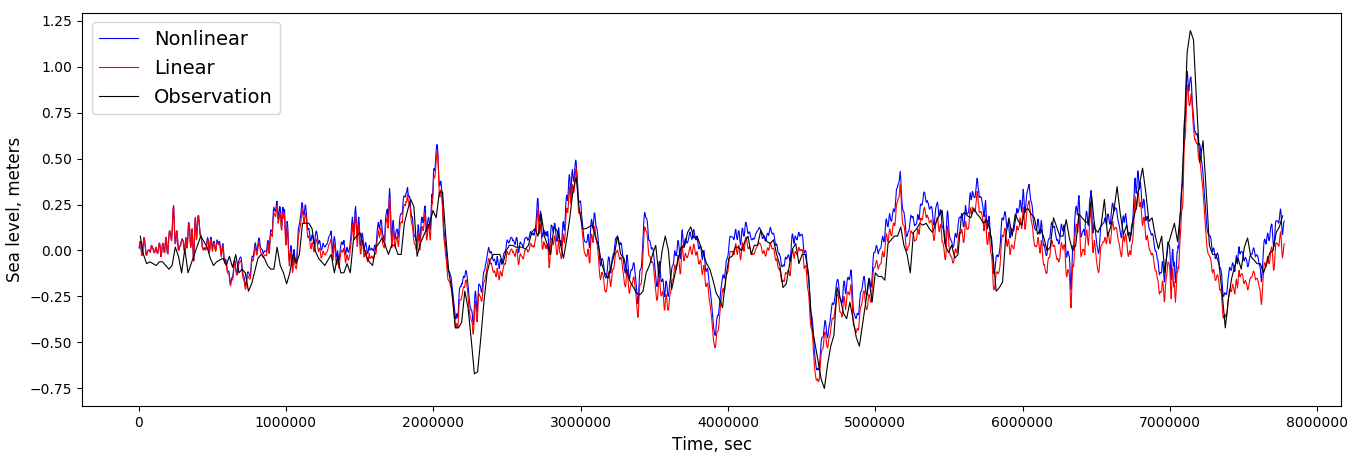
\includegraphics[width=0.85\linewidth]{EeskX.png}
	\caption{Моделирование шторма в акватории Азовского моря, сравнения уровня (метры) для поста "Ейск". 
		 Синий - нелинейные уравнения мелкой воды; красный - линеаризованные уравнения; черный - наблюдения}
	\label{fig:AS_Eesk}
\end{figure}
	
\begin{figure}[htb!]
	\center
	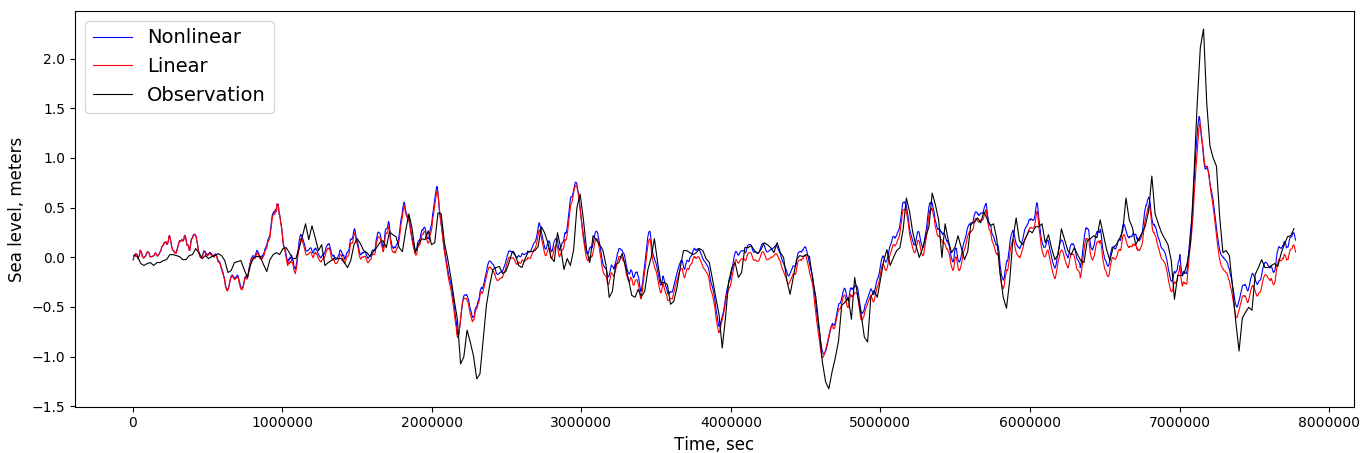
\includegraphics[width=0.85\linewidth]{TaganrogX.png}
	\caption{Моделирование шторма в акватории Азовского моря, сравнения уровня (метры) для поста "Таганрог". 
		 Синий - нелинейные уравнения мелкой воды; красный - линеаризованные уравнения; черный - наблюдения}
	\label{fig:AS_Taganrog}
\end{figure}

На рисунках \ref{fig:AS_Eesk}, \ref{fig:AS_Taganrog} продемонстрированы результаты расчетов (как по нелинейным уравнениям мелкой воды, так и по линеаризованным уравнениям) и данные наблюдений, полученные со станций "Ейск" и  "Таганрог" соответственно.
Из графиков видно, 
что результаты, полученные с помощью модели мелкой воды, хорошо согласуются с наблюдательными данными, и также было показано, что вклад нелинейности для этой задачи незначителен.

\FloatBarrier           % Глава 1
\chapter{Организация параллельных вычислений в модели мелкой воды}\label{ch:ch2}

\section{Программная архитектура модели}\label{sec:ch2/sec1}

Программная архитектура играет ключевую роль в климатических моделях, и в частности в моделях океана.
Способность модели эффективно работать на различных вычислительных системах во многом зависит от выбора правильной программной архитектуры, которая должна обеспечивать гибкость, масштабируемость и переносимость модели на различные типы вычислительных систем.
Помимо этого, гибкая программная архитектура существенно упрощает интеграцию новых компонентов и алгоритмов, что крайне важно при разработке модели.

В данной работе, для модели мелкой воды была реализована программная архитектура, основанная на принципе разделения обязанностей.
Программная архитектура заключается в том, что весь программный комплекс разделяется на три уровня: самый нижний уровень, уровень Ядра, содержит все процедуры, необходимые для вычисления уравнений мелкой воды, так называемые ядра модели; самый высокий уровень, уровень Алгоритма, отвечает за порядок вызова ядер модели и задает схему работы модели по времени; уровень Интерфейса выступает в качестве промежуточного уровня между первыми двумя и отвечает за параллельные методы и подходы, используемые в модели. 
Программные архитектуры такого типа позволяют выделить параллельные методы в обособленную часть программы (уровень Интерфейса) с целью их адаптации и гибкой настройки на целевую вычислительную систему. Причем это делается без изменений частей программы, отвечающих за вычисления уравнений мелкой воды.
Выделение параллельного ядра в отдельную часть программы также существенно упрощает разработку, отладку и оптимизацию кода под целевую вычислительную систему.

Трехуровневая программная архитектура, основанная на принципе разделения обязанностей, успешно зарекомендовала себя в модели океана NEMO (Nucleus for European Modeling of the Ocean) \cite{gmd-11-3447-2018}. 
%Исследователи планируют реализовать такую программную архитектуру во всей модели океана NEMO к 2022 году [15].

Как уже упоминалось ранее, модель полностью написана на языке Fortran, что оказывает существенное влияние на программную архитектуру и ее реализацию.
В программном коде модели широко используются модули, производные типы (классы), интерфейсы и макросы.
Отметим, что программный код для графических процессоров написан с использованием синтаксиса CUDA Fortran. 
Опишем каждый уровень программной архитектуры модели более подробно.

\subsection{Уровень Ядра}

Уровень Ядра содержит все вычислительные подпрограммы, так называемые ядра модели. Исходная непараллельная программа представляет собой набор именно таких подпрограмм.
Всего в модели мелкой воды насчитывается около 15 ядер. Ядро модели представляет собой подпрограмму, в которой производятся вычисления сеточных переменный внутри некоторой заданной расчетной области. Важно отметить, что ядро модели не содержит программного кода, отвечающего за синхронизацию данных.
Это означает, что если подпрограмма имеет несколько расчетных циклов по точкам сетки и содержит синхронизацию данных между циклами, то такая подпрограмма должна быть разбита на несколько подпрограмм (ядер модели) без синхронизации данных.
За синхронизацию данных между вызовами ядер модели отвечает уровень Интерфейса, который будет рассмотрен позже.

В случае использования процессора (CPU) для вычислений, ядро модели представляет собой двумерный цикл по точкам сетки, в котором происходит обновление значений в каждой точке сетки с использованием численных схем.
На данном уровне происходит работа с обычными двумерными массивами.
На рис. \ref{fig:kernel}а) показан общий вид ядра модели для расчета на CPU, где nx\_start, nx\_end, ny\_start, ny\_end - границы подобласти; bnd\_x1, bnd\_x2, bnd\_y1, bnd\_y2 - границы подобласти, включая внерасчетные границы; var - сеточная переменная.

\begin{figure}[!ht]
	\begin{minipage}{\linewidth}
		\centering
		\begin{lstlisting}
subroutine kernel(var)
	real(wp8), intent(inout) :: var(bnd_x1:bnd_x2, bnd_y1:bnd_y2)
	[...]
	do m = nx_start, nx_end
		do n = ny_start, ny_end
			var(m, n) = [...]
		enddo
	enddo
end subroutine
		\end{lstlisting}
		\subcaption{Программный код для расчета на CPU}
	\end{minipage}
	\begin{minipage}{\linewidth}
		\centering
		\begin{lstlisting}
attributes(global) subroutine kernel(var)
	real(wp8), intent(inout) :: var(bnd_x1:bnd_x2, bnd_y1:bnd_y2)
	[...]
	m = (blockIdx%x-1)*blockDim%x + threadIdx%x + (nx_start - 1) - 1
	n = (blockIdx%y-1)*blockDim%y + threadIdx%y + (ny_start - 1) - 1
	if (m <= nx_end + 1 .and. n <= ny_end + 1) then
		var(m, n) = [...]
	endif
end subroutine
		\end{lstlisting}
		\subcaption{Программный код для расчета на GPU}
	\end{minipage}
	\vspace{3pt}
	\caption{Уровень Ядра модели мелкой воды}
	\label{fig:kernel}
\end{figure}

В случае использования графических процессоров (GPU) для вычислений, ядро модели обновляет значения в одной точке сетки в отличие от двумерного цикла по точкам сетки при вычислениях на CPU.
Каждой точке сетки соответствует свой поток на GPU, в котором производятся вычисления.
Запуск ядра модели на GPU осуществляется потоками, охватывающими все точки расчетной области. На рис. \ref{fig:kernel}б) показан общий вид ядра модели ядра для расчета на графических процессорах.

Таким образом, в данной работе было реализовано 15 ядер модели для расчетов уравнений мелкой воды как на CPU, так и на GPU.

\subsection{Уровень Алгоритма}

На самом верхнем уровне архитектуры программного обеспечения - уровне Алгоритма - определяется порядок вызова ядер и описывается основной временной цикл модели. На этом уровне работа ведется с абстрактными структурами данных, такими как класс ocean\_type, который содержит основные сеточные переменные для уравнений мелкой воды: уровень моря, компоненты скорости, и т.д.

Пример кода этого уровня представлен на рис. \ref{fig:algorithm}. В данном примере сначала вызывается ядро для расчета уровня моря (kernel\_ssh), а затем - ядро для расчета компонент скорости (kernel\_uv). Для вызова модельных ядер используется специальная процедура envoke, являющаяся частью уровня Интерфейса, и которая будет рассмотрена далее.

\begin{figure}[!ht]
	\centering
	\begin{lstlisting}
[...]
type(ocean_type), target :: ocean_data
procedure(empty_kernel), pointer :: kernel_ssh, kernel_uv
[...]
call envoke(ocean_data%ssh, kernel_ssh)
call envoke(ocean_data%u, ocean_data%v, kernel_uv)
[...]
	\end{lstlisting}
	\vspace{3pt}
	\caption{Уровень Алгоритма модели мелкой воды}
	\label{fig:algorithm}
\end{figure}

\subsection{Уровень Интерфейса}

\begin{figure}[!ht]
	\begin{minipage}{\linewidth}в
		\centering
		\begin{lstlisting}
subroutine envoke(var, kernel)
	type(data2D_real8_type) :: var
	[...]
	!$omp do private(k) schedule(static, 1)
	do k = 1, blocks
		call kernel(var%block(k)%host)
	enddo
	!$omp end do nowait
	call sync_halo
end subroutine
		\end{lstlisting}
		\subcaption{Интерфейс для запуска расчетов на CPU}
	\end{minipage}
	\begin{minipage}{\linewidth}
		\centering
		\begin{lstlisting}
subroutine envoke(var, kernel)
	type(data2D_real8_type) :: var
	[...]
	!$omp do private(k) schedule(static, 1)
	do k = 1, blocks
		cudaSetDevice(k-1)
		call kernel<<<tGrid, tBlock>>> (var%block(k)%device)
	enddo
	!$omp end do nowait
	call copy_device_to_host	
	call sync_halo
	call copy_host_to_device
end subroutine
		\end{lstlisting}
		\subcaption{Интерфейс для запуска расчетов на GPU}
	\end{minipage}
	\vspace{3pt}
	\caption{Уровень Интерфейса модели мелкой воды}
	\label{fig:interface}
\end{figure}

Промежуточным уровнем между ядром модели и вызовом ядра модели является уровень Интерфейса, на котором реализуются все параллельные методы и подходы в модели.
В частности, на этом уровне реализуются блочная декомпозиция (раздел \ref{sec:ch2/sec2}), метод балансировки нагрузки (раздел \ref{sec:ch2/sec3}), гибридный подход с использованием технологий MPI и OpenMP (раздел \ref{sec:ch2/sec4}), гибридные подходы с использованием технологий MPI, OpenMP и CUDA (раздел \ref{sec:ch2/sec5}) реализованы на уровне Интерфейса.
Уровень Интерфейса также включает программный код для синхронизации данных между процессорами, обмена данными с внерасчетными границами и передачи данных между CPU и GPU. Уровень Ядра и уровень Алгоритма содержат описание физических процессов в модели мелкой воды - однако на этих программных уровнях ничего неизвестно о деталях параллельной реализации, которые скрыты на уровне Интерфейса. Интерфейс позволяет гибко конфигурировать и настраивать модель для различных целевых вычислительных систем без изменения программного кода на уровнях Ядра и Алгоритма.
На уровне Интерфейса происходит работа со специальными типами данных, например, с классом типа data\_2D\_real\_8", который содержит распределенные по блокам и процессорам данные. В случае использования GPU такие типы данных дублируют данные в глобальной памяти GPU, а также содержат процедуры синхронизации этих данных между CPU и GPU.
Опять же, методы организации хранения данных и детали реализации синхронизации скрыты от остальных уровней модели, отвечающих за физические процессы в модели. Это позволяет оптимизировать структуры данных под целевые вычислительные системы, без существенных изменений программного кода модели.

На рис. \ref{fig:interface}а) схематично продемонстрирована реализация интерфейса для вычисления ядер моделей на CPU с использованием подпрограммы envoke. 
Подпрограмма вызывает ядро модели для каждого блока данных и затем синхронизирует потоки OpenMP и процессы MPI (подробнее об этом подходе см. раздел \ref{sec:ch2/sec4}).

На рис. \ref{fig:interface}б) схематично продемонстрирована реализация интерфейса для вычисления ядра модели на GPU с использованием подпрограммы envoke.
Эта подпрограмма вызывает ядро модели для каждого блока данных, соответствующего своему GPU, используя специальный синтаксис CUDA.
Подпрограмма выполняет синхронизацию данных между CPU и GPU. Также синхронизируются потоки OpenMP и процессы MPI (подробнее об этом подходе см. раздел \ref{sec:ch2/sec5}).

\section{Метод декомпозиции области}\label{sec:ch2/sec2}

В качестве основного метода распараллеливания для вычислительных архитектур с распределенной памятью в модели мелкой воды используется двумерный метод декомпозиции области,
суть которого в следующем: исходная расчетная область разбивается на подобласти и каждому процессору ставится в соответствие своя подобласть.
У каждой подобласти есть внерасчетная граница толщиной в одну точку, и если процессору нужны данные с соседней подобласти,
то производится синхронизация всех процессоров, при которой заполняется внерасчетная граница каждой подобласти,
и в последующих вычислениях процессор берет эти данные со своей внерасчетной границы. Синхронизация процессоров происходит с использованием технологии MPI.

\begin{figure}[htb!]
    \center
    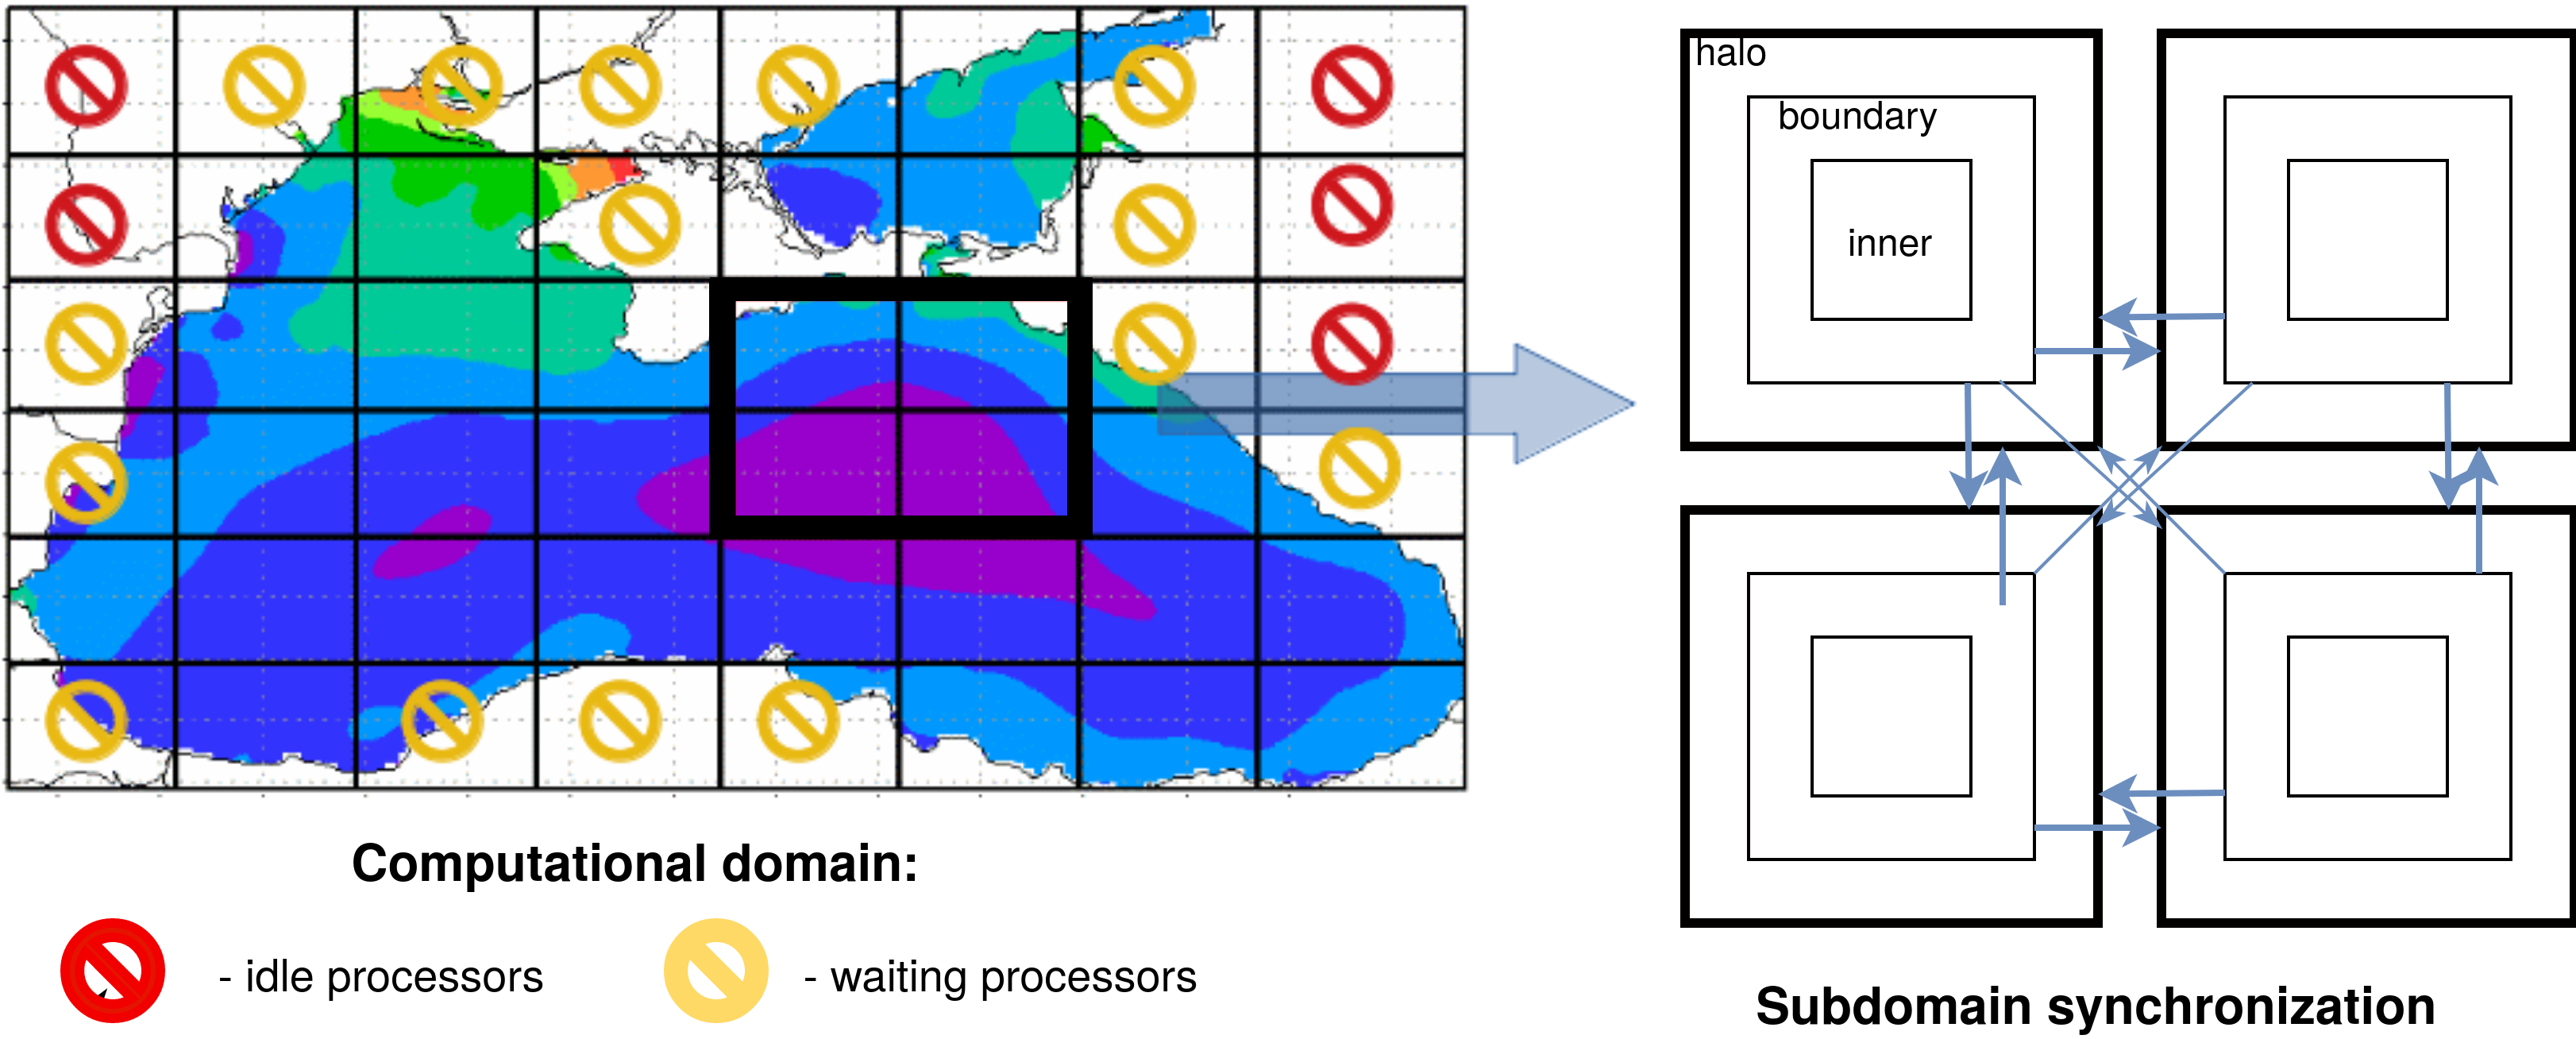
\includegraphics[scale = 0.75]{DDM.png}
    \caption{Слева: равномерное разбиение на прямоугольные подобласти, красным помечены подобласти, попадающие полностью на сушу;
    желтым помечены подобласти, загруженные менее чем на половину. Справа: механизм синхронизаций, красным показана граница каждой подобласти,
    синим показана внерасчетная граница и зеленым помечены внутренние точки подобласти.}
    \label{fig:ddm}
\end{figure}

Наиболее распространенным и легко реализуемым методом разбиения на подобласти является метод равномерного разбиения на прямоугольные подобласти,
этот метод и механизм синхронизаций представлены на рис. \ref{fig:ddm}. На рис. \ref{fig:ddm} также видно,
что из-за неоднородности акватории при таком разбиении часть подобластей полностью попадает на сушу и не участвует в вычислениях,
а часть загружена менее чем на половину из-за большого количества точек суши внутри подобластей.
При таком подходе выходит, что часть процессоров простаивает в вычислениях,
а другая часть часто находится в ожидании из-за недостаточной загруженности.

Поэтому в модели был реализован усовершенствованный метод разбиения на подобасти, так называемый блочный подход.
Суть этого подхода в следующем: исходная расчетная область равномерно разбивается на прямоугольные блоки малого размера,
и каждому процессору ставится в соответствие некоторый набор блоков, которые и формируют его расчётную подобласть, пример показан на рис. \ref{fig:LBalgo}.
Все вычисления в модели происходят по блокам, у каждого блока есть своя внерасчетная граница. Если блоки находятся внутри одной подобластии,
то при синхронизации происходит обычное копирование границы блока на внерасчетную границу соседнего блока. Если блоки находятся на соседних подоблостях,
то при синхронизации используется по-прежнему технология MPI.
Блочный подход уже успел зарекомендовать себя в таких моделях океана, как Parallel Ocean Program (POP) \cite{POP}, \cite{gmd-7-267-2014} и
HIROMB (High Resolution Operational Model for the Baltic Sea) \cite{HIROMB}.


Рассматриваемый блочный подход имеет ряд преимуществ:
\begin{itemize}
    \item Подобласти могут быть произвольными многоугольниками. Действительно, т.к. подобласть состоит из набора блоков малого размера, то можно формировать подобласти довольно произвольной формы. Это свойство позволяет проводить метод балансировки нагрузки вычислений на процессоры, формируя подобласти примерно одинаковой загруженности, о чем будет более подробно написано в следующем разделе.
    \item Эффективная работа с кэш памятью. Выбирая блок малого размера, можно получить прирост в производительности за счет эффективной работы с памятью.
    Для гидродинамических моделей это свойство крайне важно, т.к. любое вычисление на сетке сопровождается большим количеством обращений в память.
    Если блоки, для которых проводятся вычисления, помещаются полностью в кэш память, то  многочисленные обращения в память перестают быть такими дорогостоящими,
    и можно ожидать значительный прирост в производительности.
\end{itemize}

Также блочный подход имеет недостаток:
\begin{itemize}
    \item Дополнительные затраты на копирование внерасчетной границы блоков при синхронизации.
\end{itemize}

В разделе с вычислительными экспериментами будет показано, что при малом размере блоков эффективная работа с кэш памятью компенсирует затраты на копирование при синхронизации, и поэтому этот недостаток можно считать не таким существенным.

\section{Метод балансировки нагрузки вычислений}\label{sec:ch2/sec3}

Под балансировкой нагрузки вычислений имеется в виду такое распределение подзадач между процессорами, 
которое обеспечивает наиболее равномерно распределенную нагрузку на процессоры и минимальные затраты на передачу данных между ними.
Методы балансировки нагрузки вычислений позволяют снизить время простоя отдельных процессоров
и тем самым повысить эффективность параллельной программы, что существенно важно при решении задач 
на высокопроизводительных вычислительных системах.
Балансировка нагрузки вычислений особенно актуальна в задачах моделирования циркуляции океана и моделирования цунами,
потому что из-за наличия берегов и островов в этих задачах равномерное разбиение будет давать особенно несбалансированные подобласти, как будет показано далее в работе.
Тут важно отметить, что оптимальность разбиения для мелкой воды будет точно соответствовать оптимальности для трехмерной сигма-модели INMOM, 
так как количество расчетных уровней по глубине в сигма-модели одинаково для всех точек сетки по горизонтали. 

Существуют два основных способа балансировки нагрузки: методы, основанные на графах, и геометрические методы. 
Методы, основанные на графах, реализованы, например, в библиотеках METIS и parMETIS \cite{METIS} и пользуются довольно большой популярностью. 
Такие методы представляют расчётную область в виде графа, в котором вершины соответствуют узлам сетки, а рёбра - связям между узлами.
Однако у них есть недостаток - это их сложность для программной реализации. 
Поэтому, как альтернатива этим методам, в задачах моделирования океана часто используются 
геометрические методы, такие как разбиение вдоль фрактальной кривой \cite{Dennis2007}, рекурсивной бисекции \cite{Rantakokko1998} и др. 
Такие методы основаны на том, что каждый узел имеет связи со своими соседями.
Геометрические методы дают разбиение хорошего качества и это хорошая альтернатива METIS/parMETIS для многих задач. 
    
В данной работе рассматривается один из геометрических методов балансировки нагрузки: метод разбиения вдоль фрактальной кривой, который
уже успел зарекомендовать себя во многих работах, например, в \cite{Dennis2007}, \cite{Hui2017}. 

В работе показано, что данный метод показывает хорошие результаты применительно к решению уравнений мелкой воды, а также показано сравнение этого метода с METIS.

\subsection{Метод разбиения вдоль фрактальной кривой}

Метод разбиения вдоль фрактальной кривой основывается на фрактальных кривых заполняющих пространство (Space-Filling Curve, SFC).
Такие кривые преобразуют d-мерное пространство в одномерное с сохранением свойства локальности,
т.е. соседние элементы в d-мерном пространстве преобразуются в соседние элементы в одномерном пространстве.
Существует целое множество кривых, заполняющих пространство \cite{SFC1994}. 
На практике используются кривые Пеано и их частные случаи - кривые Гильберта и кривые Мортона \cite{Dennis2007}, \cite{Hui2017}, \cite{gmd-7-267-2014}.
В рамках применения метода разбиения вдоль фрактальной кривой к решению нелинейных уравнений мелкой воды, 
в данной работе будут рассматриваться кривые Гильберта в двумерном пространстве.
    
Кривые Гильберта используются для преобразования двумерной области с размерами $nb_x \times nb_y$ в кривую, где
$nb_x \times nb_y = 2^n$ и $n$ - это целое число, которое называется индексом кривой Гильберта.
Рис. \ref{fig:HC} показывает пример кривых Гильберта с индексами 2, 4, 8.
    
    \begin{figure}[htb!]
    \begin{minipage}[h]{0.3\linewidth}
    \center{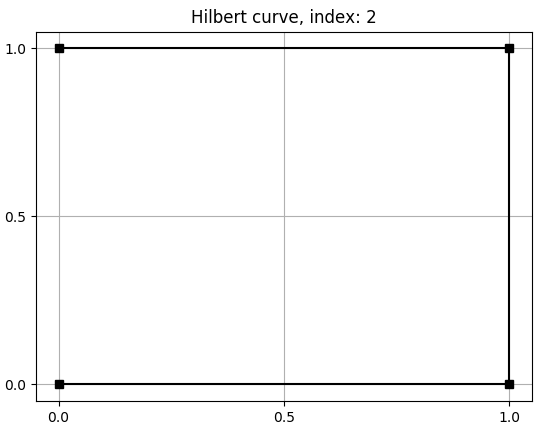
\includegraphics[scale = 0.4]{HC_index2.png}}
    \end{minipage}
    \hfill
    \begin{minipage}[h]{0.3\linewidth}
    \center{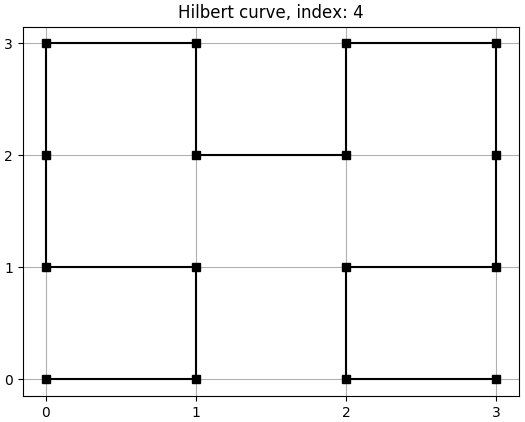
\includegraphics[scale = 0.4]{HC_index4.png}}
    \end{minipage}
    \hfill
    \begin{minipage}[h]{0.3\linewidth}
    \center{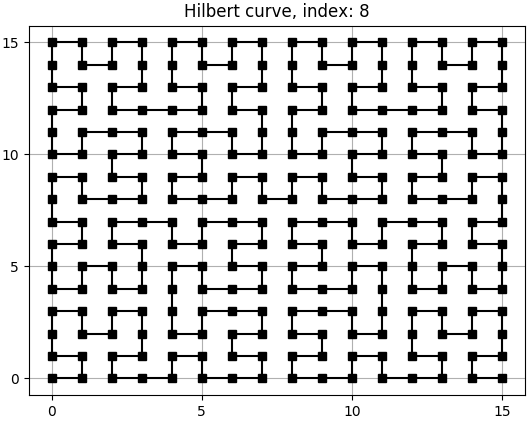
\includegraphics[scale = 0.4]{HC_index8.png}}
    \end{minipage}
    \caption{Кривые Гильберта с индексами 2, 4 и 8 соответственно}
    \label{fig:HC}
    \end{figure}
    
Алгоритм балансировки нагрузки с помощью кривых Гильберта следующий. 
Предварительно вся расчётная область с размерами $nx \times ny$ точек равномерно разбивается
на сетку с размерами $nb_x \times nb_y = 2^n$, состоящую из прямоугольных блоков.
Для каждого блока рассчитывается значение загруженности блока $w_i$ как сумма всех точек, которые не лежат на суше.
Далее, на сетке блоков проводится кривая Гильберта, которая переводит
двумерное пространство блоков в одномерное.
Разбиение на подобласти происходит вдоль кривой и причем таким образом, чтобы
подобласти имели примерно одинаковую сумму загруженности блоков.
Затем каждому процессору ставится в соответствие его подобласть, на которой он проводит вычисления.
Блоки, которые полностью состоят из точек на суше (т.е. загруженность которых $w_i = 0$),
в распределении по процессорам и в дальнейших вычислениях не участвуют. 
На рис. \ref{fig:LBalgo} наглядно показаны шаги описанного алгоритма. 

    
    \begin{figure}[htb!]
    \begin{minipage}[h]{0.32\linewidth}
    \center{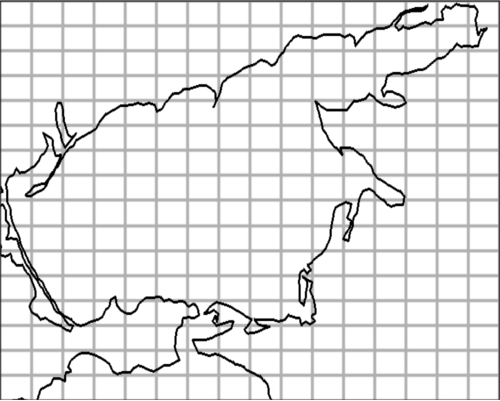
\includegraphics[width=1.0\linewidth, height=140pt]{blockgrid.png}}
    \end{minipage}
    \hfill
    \begin{minipage}[h]{0.32\linewidth}
    \center{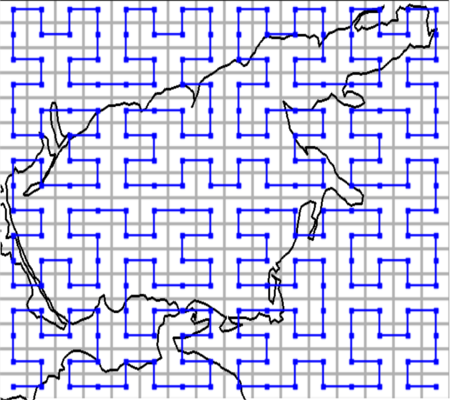
\includegraphics[width=1.0\linewidth, height=140pt]{blockhilbert.png}}
    \end{minipage}
    \hfill
    \begin{minipage}[h]{0.32\linewidth}
    \center{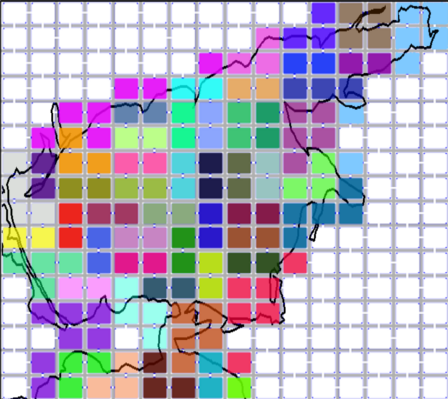
\includegraphics[width=1.0\linewidth, height=140pt]{hilbertLB.png}}
    \end{minipage}
    \caption{Алгоритм балансировки нагрузки с помощью кривых Гильберта. 1) Равномерное разбиение на блоки 
             2) На сетке блоков проводится кривая Гильберта
             3) Блоки объединяются в подобласти вдоль кривой Гильберта.
                Каждому процессору ставится в соответствие его подобласть. }
    \label{fig:LBalgo}
    \end{figure}
    
    
Пример такого разбиения в сравнении с равномерным разбиением без балансировки нагрузки и с разбиением, полученным с помощью библиотеки METIS,
приведён на рис. \ref{fig:map_uniform_hilbert_metis} для акватории Азовского моря с размерами $1525 \times 1115$ точек, 
сетка блоков $32 \times 32$.
Чёрным цветом на рисунке изображены блоки, состоящие только из точек на суше и которые не
участвуют в вычислениях.
    
    \begin{figure}[htb!]
    \begin{minipage}[h]{0.32\linewidth}
    \center{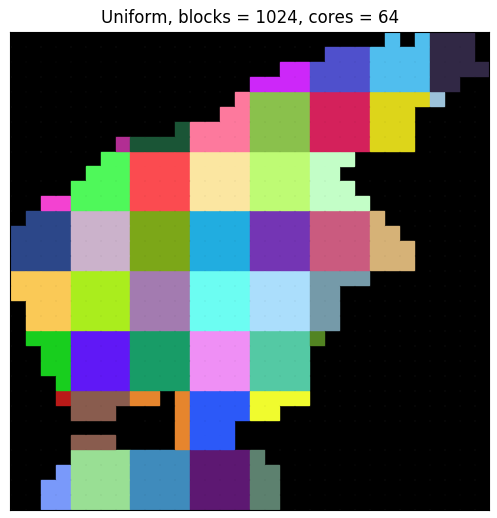
\includegraphics[width=1.0\linewidth]{1024b_64p_u.png}}
    \end{minipage}
    \hfill
    \begin{minipage}[h]{0.32\linewidth}
    \center{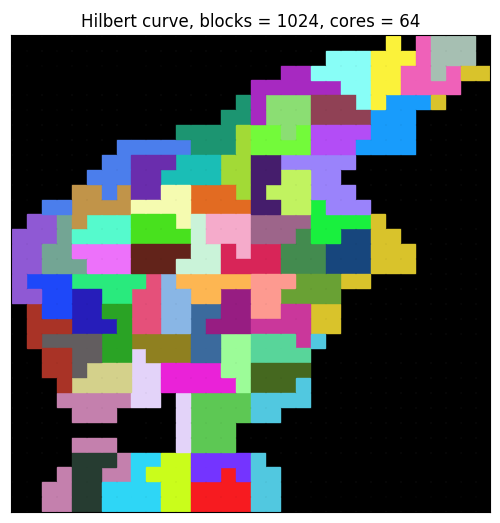
\includegraphics[width=1.0\linewidth]{1024b_64p_h.png}}
    \end{minipage}
    \hfill
    \begin{minipage}[h]{0.32\linewidth}
    \center{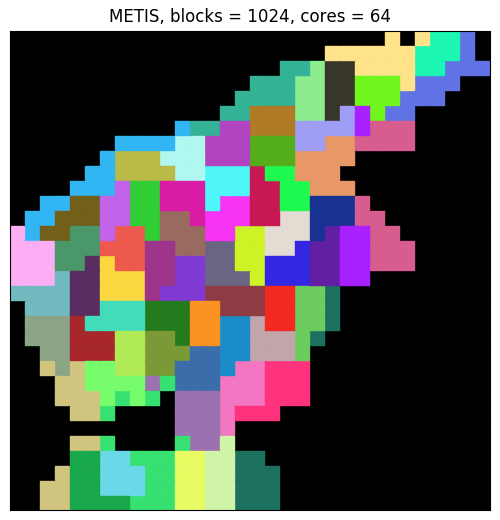
\includegraphics[width=1.0\linewidth]{1024b_64p_metis.png}}
    \end{minipage}
    \caption{Различные разбиения для 64 процессоров, 1024 блоков. 1) Равномерное разбиение 2) Метод разбиения c использованием кривой Гильберта 
             3) Разбиение полученное с помощью METIS}
    \label{fig:map_uniform_hilbert_metis}
    \end{figure}
    
Следует отметить, что у описанного метода балансировки нагрузки вычислений с использованием кривых Гильберта есть несколько недостатков:
ограничение на сетку блоков (сетка должна быть размерами $nb_x \times nb_y = 2^n$); 
большое количество пересылок при большом количестве блоков на процессоре.

\subsection{Метрики качества разбиения}
\label{sec:ch2/sec3/lb}

Для того, чтобы понимать качество полученного разбиения, полезно иметь некоторые метрики \cite{Dennis2007}, \cite{Hui2017}.
В этой части мы введем пару метрик качества разбиения. Предположим, что разбиение происходит на $k$ подобластей для $p$ процессоров.
Введём первую метрику $LB$, которая будет отвечать за сбалансированность разбиения с точки зрения нагрузки вычислений на процессоры:

\begin{equation} \label{eq:LB}  
    \displaystyle { LB = \frac{\max_{1 \leq i \leq k} W_i}{\frac{1}{p}\sum_{i=1}^k W_i} }
\end{equation} 

где $\max_{1 \leq i \leq k} W_i$ - максимальная загруженность $i$ подобласти, $\sum_{i=1}^k W_i$ - полная загруженность всей расчётной области.
Эта величина показывает отношение максимальной загруженности подобласти в разбиении к оптимальной загруженности.
Значение $LB = 1$ соответствует идеально сбалансированному разбиению. 
    % (с точки зрения нагрузки вычислений на процессоры)
    
Введём также вторую метрику $r_M$, которая будет отвечать за качество разбиения с точки зрения коммуникаций между соседними подобластями:

\begin{equation} \label{eq:RM}  
    \displaystyle { r_M = max_{1 \leq i \leq k} \frac{e_i}{s_i} }
\end{equation} 

где $e_i$ - количество узлов $i$ подобласти, которые соседние для некоторой другой подобласти, $s_i$ - количество всех узлов $i$ подобласти.
Эта величина показывает максимальное отношение периметра к объему подобласти. 
Для разбиений с завышенной величиной $r_M$ время на коммуникации между процессорами становится доминирующим.
%Чем это отношение меньше - тем происходит меньше коммуникаций и больше вычислений для подобласти. 
Библиотека METIS по умолчанию пытается построить разбиение, минимизирующее именно такую метрику.
   
Было проведено сравнение метода балансировки нагрузки вычислений, использующего кривую Гильберта, с библиотекой METIS.
В таблице \ref{tab:LB} приведены метрики качеств полученных разбиений. 
На рис. \ref{fig:map_uniform_hilbert_metis} показаны разбиения для 64 ядер. 
Методы рассматривались на сетках блоков: по 8 блоков на ядро для 32 и 128 ядер и по 16 блоков на ядро для всех остальных. 
Видно, что метод балансировки с использованием кривых Гильберта даёт разбиения, очень близкие к разбиениям METIS, как по значениям метрик качества разбиения, так и по значениям полученного ускорения параллельной программы.    
Для 256 ядер видно даже, что по всем метрикам качества разбиение, полученное с помощью кривых Гильберта, немного лучше чем METIS.
Поэтому можно сделать вывод, что для данной задачи метод балансировки нагрузки вычислений с использованием кривой Гильберта - это хорошая альтернатива библиотеке METIS.   
    
%В целом, для рассмотренной задачи выяснилось, что можно использовать как балансировку нагрузки с использованием кривых Гильберта так и METIS. 
Отметим, что метод балансировки с использованием кривых Гильберта строит разбиения в несколько раз быстрее METIS, но для рассматриваемой задачи это незначительно, т.к. расчетное время на порядок больше чем время построения разбиения. 
Однако, алгоритм балансировки с использованием кривых Гильберта будет давать существенные преимущества по сравнению с METIS, когда задача будет упираться во время построения разбиения, например, на очень большой расчетной области и с адаптивной сеткой.
Также описанный алгоритм балансировки предпочтительнее чем METIS, так как он реализован непосредственно в модели и его реализация довольно простая в отличие от того, что реализовано в METIS. METIS - это библиотека для разбиений вообще произвольного вида, в ней реализованы довольно громоздкие методы, основанные на графах. А балансировка с использованием кривых Гильберта - это геометрический метод, который сильно проще и очень хорошо подходит именно для рассматриваемой задачи.  
Используя описанный алгоритм балансировки нагрузки, у модели не будет привязки к сторонней библиотеке, поэтому дальнейшая разработка, поддержка и улучшения этого инструмента будут легче чем работа с METIS.
    
%Из рисунка видно, что оптимальной сеткой блоков для данной задачи является сетка с размерами $32 \times 32$.
%При такой сетке для данной задачи размер каждого блока составляет 1660 точек.
%Ухудшение масштабируемости для сетки блоков с размерами $64 \times 64$ можно объяснить тем, что
%при таком большом количестве блоков коммуникационные задержки на перессылки между блоками
%становятся существенными, хоть и подобласти при таком разбиении будут более сбалансированными (см. таблицу).
    
\begin{table}[]
    \caption{a) Метрика $LB$ для различных разбиений b) Метрика $r_M$ для различных разбиений}\label{tab:LB}
    \begin{subtable}{.5\linewidth}
    \centering
    \caption{}
    \resizebox{0.9\textwidth}{!}
    {
    \begin{tabular}{|l|l|l|l|l|l|}
    \hline
    Cores     & 4      & 16     & 64     & 128    & 256    \\ 
    \hline
    Blocks 
    per core  & 16     & 16     & 16     & 8      & 16     \\
    \hline
    Uniform   & 1.5278 & 2.3872 & 2.4025 & 2.4025 & 2.4025 \\
    \hline
    Hilbert   & 1.0535 & 1.0655 & 1.0640 & 1.2012 & 1.0651 \\
    \hline
    METIS     & 1.0384 & 1.0511 & 1.1080 & 1.1714 & 1.1006 \\
    \hline
    \end{tabular}
    }
    \end{subtable}
    \begin{subtable}{.5\linewidth}
    \centering
    \caption{}
    \resizebox{0.92\textwidth}{!}
    {
	\begin{tabular}{|l|l|l|l|l|l|}
    \hline
    Cores     & 4       & 16      & 64      & 128     & 256     \\ 
    \hline
    Blocks 
    per core  & 16      & 16      & 16      & 8       & 16      \\
    \hline
    Uniform   & 0.311\% & 1.248\% & 2.501\% & 3.554\% & 5.003\% \\
    \hline
    Hilbert   & 1.279\% & 2.558\% & 5.417\% & 7.300\% & 10.88\% \\
    \hline
    METIS     & 0.716\% & 2.501\% & 5.185\% & 8.719\% & 12.13\% \\
    \hline
    \end{tabular}
    }
    \end{subtable}
\end{table}

\section{Гибридная модель параллельного программирования для использования на многопроцессорных системах}\label{sec:ch2/sec4}

Гибридные модели, сочетающие в себе технологии передачи сообщений MPI для архитектур с распределенной памятью и многопоточной обработки данных OpenMP для архитектур с общей памятью, становятся все более популярными, поскольку современные высокопроизводительные вычислительные системы представляют собой набор многопроцессорных систем с общей памятью (вычислительных узлов), объединенных в единую коммуникационную сеть. 
Создание моделей, эффективно использующих ресурсы таких вычислительных систем, является актуальной задачей на сегодняшний день \cite{gmd-11-1799-2018}.
	    
Узкое место в рассматриваемой модели мелкой воды - это синхронизации MPI между процессорами, т.к.  при увеличении числа вычислительных узлов возрастают накладные расходы на синхронизации из-за высокой нагрузки на сеть. Можно уменьшить синхронизации, и тем самым уменьшить нагрузку на сеть, если использовать OpenMP для распараллеливания на общей памяти внутри узла. Это так называемый гибридный подход. Если при использовании только технологии MPI, в так называемом чистом MPI подходе, для каждого ядра на узле создается отдельный MPI процесс, то в гибридном MPI + OpenMP подходе на каждый узел создается только один MPI процесс, и для каждого ядра создаются отдельные потоки. Гибридные подходы в последнее время становятся все более актуальными и используются во многих гидродинамических моделях \cite{Liu2019ParallelIA}, \cite{Afzal_Ansari_Faizabadi_Ramis_2016}, \cite{MPIOpenMP2017},  \cite{Mortikov2016}.

	\begin{figure}[htb!]
    \center
    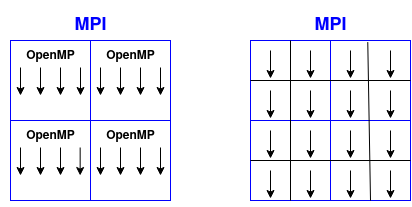
\includegraphics[scale = 0.5]{openmp.png}
    \caption{Гибридные MPI + OpenMP подходы. Слева векторный подход; справа задачный подход.}
    \label{fig:openmp}
    \end{figure}

Есть два подхода при использовании технологии OpenMP для распараллеливания на общей памяти \cite{Wellein2003}. Первый и наиболее распространенный подход называется векторным подходом (vector based). При этом подходе происходит распараллеливание по потокам всех вычислений в модели по подобласти, как схематично показано слева на рис. \ref{fig:openmp}. Т.е. каждому MPI процессу соответствует некоторая подобласть, и все OpenMP потоки существуют и проводят вычисления внутри этой общей для них подобласти. Этот подход легко реализуем, но демонстрирует малую производительность во многом из-за того, что потоки OpenMP неэффективно используют кэш память при работе на общей памяти.

Второй подход называется задачным подходом (task based). Главная идея в этом подходе заключается в том, чтобы использовать метод декомпозиции области для потоков OpenMP, т.е. ставить каждому потоку в соответствие некоторую подобласть. При таком подходе каждый поток существует и проводит вычисления на своей собственной подобласти, как схематично показано справа на рис. \ref{fig:openmp}. За основу гибридного MPI + OpenMP подхода в модели мелкой воды был взят именно задачный подход. Блоки из разбиения распределяются как по процессам MPI, так и по потокам OpenMP. Распределение блоков по MPI процессам происходит с использованием метода балансировки нагрузки вычислений, описанного в предыдущем разделе, и далее происходит распределение блоков по OpenMP потокам внутри каждого MPI процесса с использованием жадного алгоритма следующим образом: все доступные блоки MPI процесса сортируются по величине загруженности и далее в этом порядке по одному распределяются на все доступные потоки внутри MPI процесса. Такой алгоритм, при условии, что количество блоков в разбиении велико, обеспечивает равномерную нагрузку вычислений по всем доступным потокам в вычислительной системе.

В разделе с вычислительными экспериментами будет проведено сравнение двух описанных гибридных подходов MPI + OpenMP и продемонстрировано, что задачный подход во многом эффективнее векторного подхода. Здесь же отметим, что именно задачный OpenMP подход используется в широко известных моделях атмосферы WRF (Weather Research and Forecasting Model) \cite{WRF2016} и океана ROMS (Regional Ocean Modeling System) \cite{Liu2019ParallelIA}, \cite{SHCHEPETKIN2005347}.

Отметим также следующие особенности реализованного гибридного подхода с использованием технологий MPI и OpenMP:

\begin{itemize}
\item У каждого процессора есть буфер для MPI обмена данными c соседними процессорами, в котором имеется место под хранение данных со всех границ блоков подобласти, необходимых для перессылки на соседние процессоры. Синхронизация между подобластями происходит с использованием этого буфера и неблокирующими вызовами MPI, причем синхронизация выполняется одним потоком.

\item При синхронизации копирование границы блоков во внерасчетную границу соседних блоков и в буфер для MPI обмена происходит параллельно всеми потоками OpenMP.

\item Для OpenMP параллельный регион создается в начале запуска модели и существует до конца расчета, что минимизирует временные затраты на инициализацию потоков в модели.
%, как было бы если параллельные регионы создавались и уничтожались динамически в течении расчета модели.

\item Инициализация всех данных происходит в параллельном регионе OpenMP. Это обеспечивает то, что страница памяти выделяется с узла того потока, который первый к ней обратился (first-touch policy). При таком подходе потоки эффективнее работают с памятью в NUMA-системах (Non Uniform Memory Access), в которых доступ в память чужого узла занимает существенно больше времени, чем доступ в память своего узла. 

\item Балансировка нагрузки вычислений по потокам происходит в начале расчета, и далее всюду используется статическое планирование OpenMP потоков по блокам, т.е. используется schedule(static). При динамическом планировании, т.е. при использовании schedule(dynamic), имеются накладные расходы  и происходит менее эффективная работа с памятью, чем при статическом планировании.
 
\item Всюду, где это возможно, используется nowait для параллельных секций OpenMP, чтобы минимизировать точки синхронизации потоков.
\end{itemize}


\section{Гибридные модели параллельного программирования для использования на гетерогенных вычислительных системах}\label{sec:ch2/sec5}

Графические процессоры становятся все более популярными в качестве выбора целевой архитектуры для проведения моделирования климата. 
Имеются примеры успешной адаптации моделей атмосферы и океана для использования на GPU, в том числе моделей мелкой воды \cite{plosSW}, \cite{VOLNA}, \cite{gpuPOM}.

В данной работе, модель мелкой воды была полностью адаптирована для выполнения расчетов на GPU, использую технологию CUDA. 
Было всего адаптировано 15 ядер модели (см. Уровень Ядра модели - раздел \ref{sec:ch2/sec1}) для расчетов на GPU.
Для обеспечения возможности использования различных параллельных шаблонов программирования для вычислений на GPU были произведены модификации в уровне Интерфейс программной архитектуры.
Важно отметить два ключевых аспекта в реализации ядер модели для расчетов на GPU: первым является использование двойной точности во всех вычислениях, а вторым - отсутствие оптимизаций памяти.
Последнее означает, что в ядрах модели не реализованы оптимизации размещения данных на GPU, в частности, не используются общая и текстурная памяти. 
Все обращения к памяти в ядрах модели выполняются непосредственно к глобальной памяти GPU. 
Современные поколения GPU менее чувствительны к оптимизации размещения данных по сравнению с более старыми поколениями, в основном благодаря улучшениям кэшей глобальной памяти, как показано в работе \cite{CUDAopt}.
Авторы данной статьи рассмотрели различные приложения, включая решатель вычислительной гидродинамики, и показали, что использование различных оптимизаций памяти на современных поколениях GPU (Pascal, Volta) в целом не приводит к такому же увеличению производительности, как на более старых поколениях GPU.
Тем не менее, эти результаты следует рассматривать только как часть общей картины. 
Кроме того, мы реализовали ядра модели для вычислений на GPU с минимальными изменениями кода, и адаптацию на GPU можно дополнительно автоматизировать с использованием макросов, как это сделано в работе \cite{gmd-11-3447-2018}.

Реализация на GPU была адаптирована для поддержки блочного подхода в модели мелкой воды, которое успешно использовалось при вычислениях на CPU. 
Благодаря блочному подходу возможно балансирование нагрузки вычислений на GPU.
Было реализовано три параллельных шаблона программирования для вычислений на GPU: синхронный шаблон MPI-CUDA, асинхронный шаблон MPI-OpenMP-CUDA, шаблон MPI-OpenMP-CUDA с использованием нескольких GPU на вычислительном узле.
Эти шаблоны схематично представлены на рисунке \ref{fig:patterns} в сравнении с параллельными шаблонами программирования для вычислений на CPU также реализованными в модели.

\begin{figure}[!ht]
	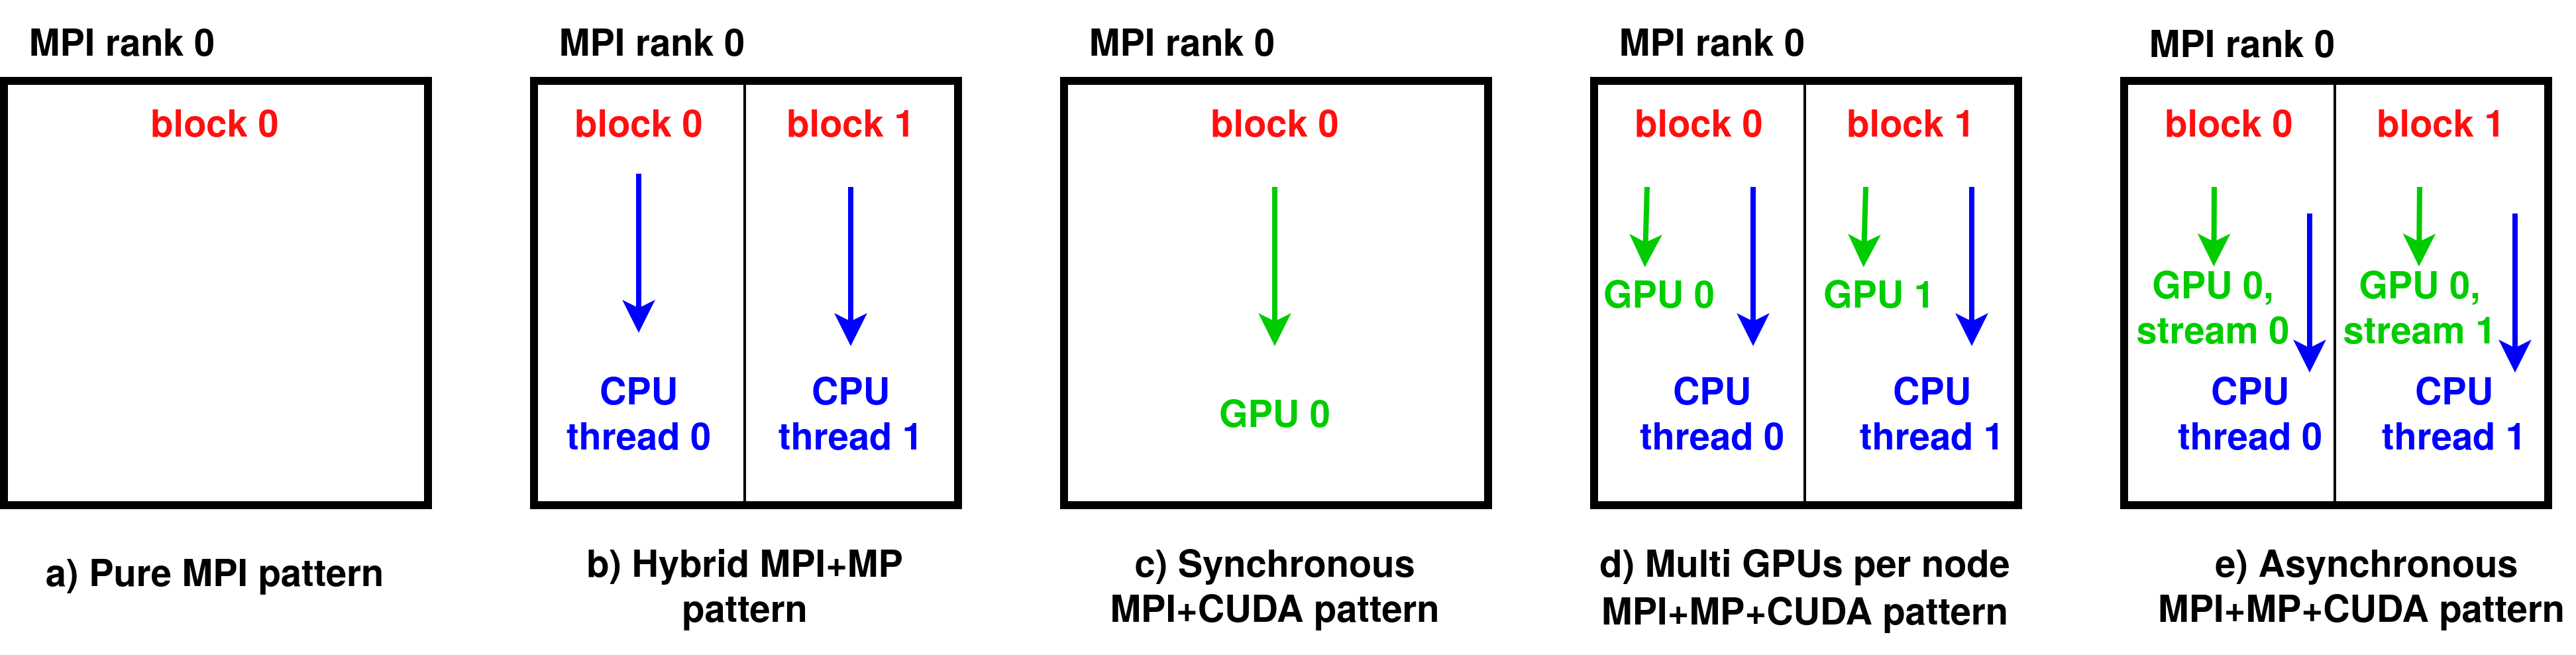
\includegraphics[width=\linewidth]{CPU_GPU_patterns.png}
	\vspace{3pt}
	\caption{Параллельные шаблоны программирования реализованные в модели}
	\label{fig:patterns}
\end{figure}

Обратите внимание, что все эти вычислительные шаблоны не вызывали сложностей при реализации, поскольку архитектура программного обеспечения основана на разделении обязанностей.
Все модификации кода были выполнены на уровне Интерфейс - без модификаций на уровнях Ядро и Алгоритм.
Опишем каждый из параллельных шаблонов программирования для вычислений на GPU более подробно.

\subsubsection{Синхронный шаблон вычислений MPI-CUDA}

В данном подходе каждому процессу MPI назначается подобласть, содержащая только один блок, и один GPU для вычислений, как показано на рисунке \ref{fig:patterns}. 
Вычисления на подобласти выполняются полностью на GPU с использованием технологии CUDA. 
После выполнения вычислений ядра модели на GPU происходит синхронизация процессоров следующим образом:

\begin{enumerate}
\item Граничные точки подобласти синхронно передаются с GPU на CPU, то есть используется блокирующая передача данных.
\item Процессы MPI синхронизируются, и внерасчетная граница каждой подобласти обновляется. Синхронизация MPI выполняется полностью на CPU.
\item Обновленная внерасчетная граница передается обратно с CPU на GPU. Передача данных также синхронная.
\end{enumerate}

Этот шаблон поддерживает вычисления на нескольких GPU, предполагая только один блок и GPU на процесс MPI, и не поддерживает блочный подход. 
Таким образом, в данном подходе отсутствует балансировка нагрузки вычислений на GPU.

\subsubsection{Асинхронный шаблон вычислений MPI-OpenMP-CUDA}

В данном шаблоне поддерживается блочный подход для вычислений на GPU. 
Каждому процессу MPI назначается подобласть, содержащая несколько блоков, и создаются потоки OpenMP и потоки CUDA для каждого блока подобасти в процессе MPI, как показано на рисунке \ref{fig:patterns}. 
Ядро модели запускается для вычислений на GPU для каждого блока подобласти следующим образом:

\begin{enumerate}
\item Каждый поток OpenMP асинхронно запускает ядро модели на GPU для блока подобласти. Запуск выполняется в потоке CUDA, соответствующем потоку OpenMP.
\item Каждый поток OpenMP асинхронно передает граничные точки с GPU на CPU блока подобласти. Передача данных выполняется в потоке CUDA, соответствующем потоку OpenMP.
\item Все потоки CUDA и потоки OpenMP синхронизируются.
\item Процессы MPI синхронизируются, и внерасчетные границы каждого блока подобласти обновляются. Синхронизация MPI выполняется полностью на CPU.
\item Каждый поток OpenMP асинхронно передает обновленные внерасчетные границы с CPU на GPU блока подобласти. Передача данных выполняется в потоке CUDA, соответствующем потоку OpenMP.
\end{enumerate}

Поскольку современные GPU имеют отдельные управляющие элементы для выполнения ядер и передачи данных, этот шаблон вычислений организует асинхронную передачу данных и перекрывает выполнение ядра на GPU с передачей данных между CPU и GPU в разных потоках CUDA. 
На рисунке \ref{fig:GPUpatterns} схематически показаны шаги этого шаблона вычислений сравнительно с синхронным шаблоном MPI-CUDA.
Можно видеть, что передача данных перекрывается с выполнением ядра по времени для асинхронного шаблона MPI-OpenMP-CUDA.
Этот шаблон вычислений полностью гибриден и разработан для более эффективных вычислений на вычислительных узлах с одним GPU на узел по сравнению с синхронным шаблоном MPI-CUDA.

\begin{figure}[!ht]
	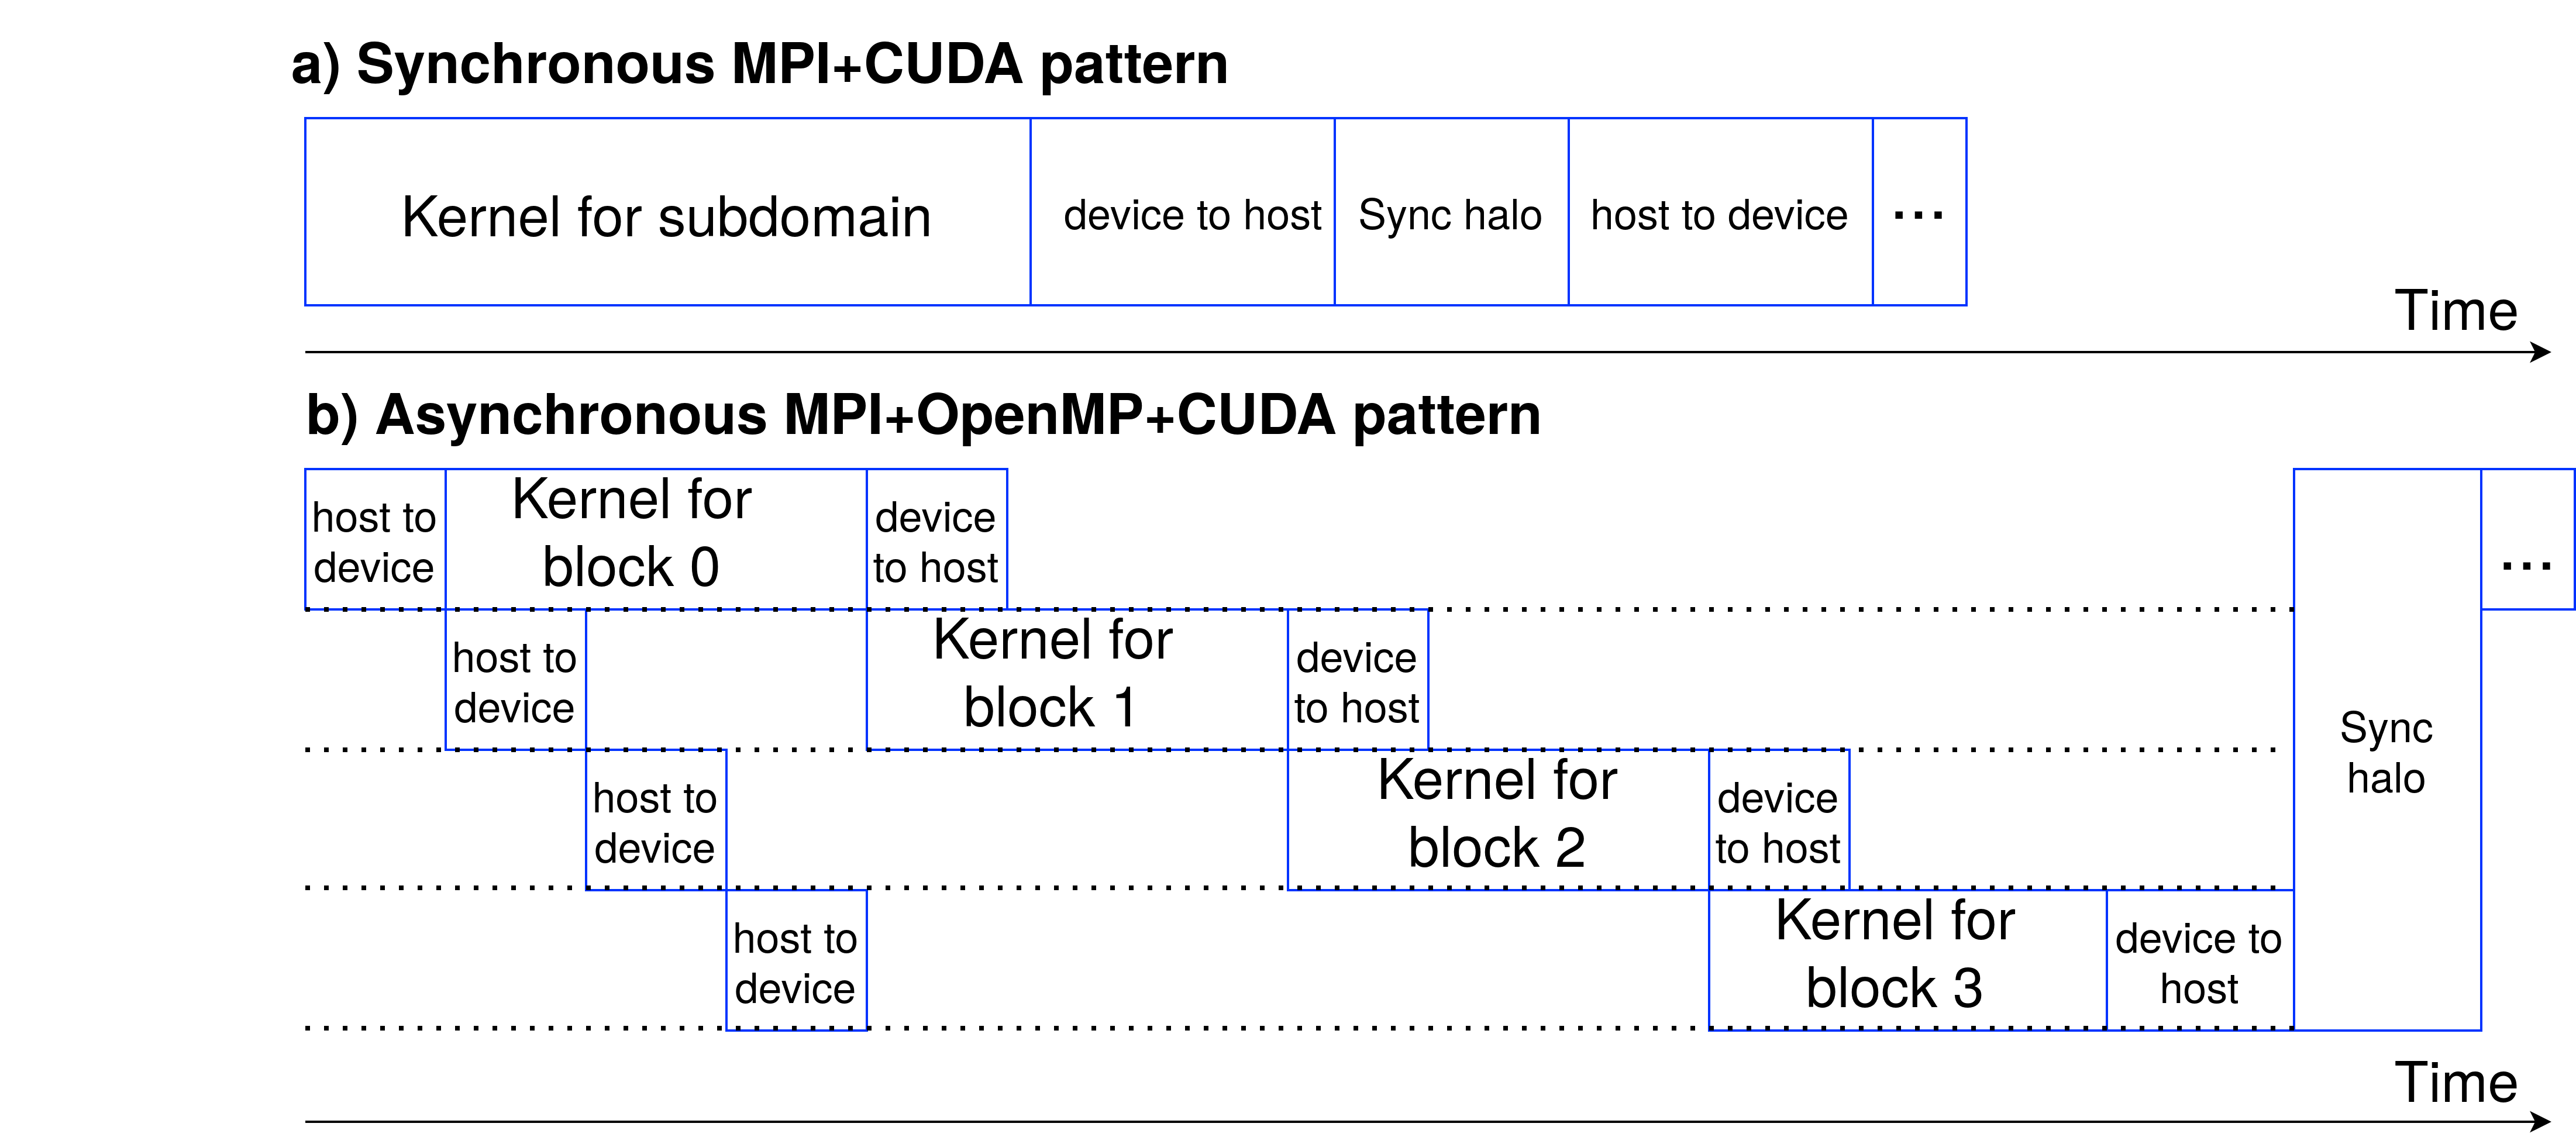
\includegraphics[width=\linewidth]{GPUpatterns.png}
	\vspace{3pt}
	\caption{Синхронный шаблон вычислений MPI-CUDA и асинхронный шаблон вычислений MPI-OpenMP-CUDA}
	\label{fig:GPUpatterns}
\end{figure}

\subsubsection{Шаблон MPI-OpenMP-CUDA с использованием нескольких GPU на вычислительном узле}

Этот шаблон также поддерживает блочный подход для вычислений на GPU, но иначе, чем асинхронный шаблон MPI-OpenMP-CUDA.
Каждому процессу MPI назначается несколько блоков и потоков OpenMP, столько, сколько доступно GPU на узле. 
Следовательно, каждый GPU, управляемый одним потоком OpenMP, содержит один блок подобласти на узле. 
Потоки OpenMP независимо запускают ядра CUDA, что позволяет эффективно использовать каждый доступный GPU на узле. 
Синхронизация организована, как и в шаблоне MPI-CUDA, но с синхронизацией GPU на узле и сбором граничных точек между GPU для синхронизации процессов MPI. Этот подход является полностью гибридным и разработан для вычислений на вычислительных узлах с несколькими GPU на узле.

\FloatBarrier
           % Глава 2
\chapter{Исследование производительности и масштабируемости моделей мелкой воды и общей циркуляции океана INMOM}\label{ch:ch3}

\section{Тестирование модели мелкой воды на суперкомпьютере Ломоносов-2}\label{sec:ch3/sec1}

Были проведены эксперименты на суперкомпьютере Ломоносов-2 в Московском государственном университете имени Ломоносова %\сite{L2}.
Этот суперкомпьютер является полностью гетерогенной вычислительной системой и на сегодняшний день является одним из наиболее производительных суперкомпьютеров в России согласно списку TOP500 \cite{TOP500}.
Мы проводили наши численные эксперименты на разделах Pascal и Volta этого суперкомпьютера, которые оборудованы современными графическими процессорами (GPU) на узлах. Раздел Pascal включает 160 узлов, на каждом из которых установлен один процессор Intel Xeon Gold 6126 с тактовой частотой 2.60 ГГц (12 ядер) и два графических процессора Nvidia Tesla P100; раздел Volta включает 16 узлов, на каждом из которых  установлен процессор Intel Xeon Gold 6126 с тактовой частотой 2.60 ГГц (12 ядер) и два графических процессора Nvidia Tesla V100. 
Для компиляции программного кода мы использовали компилятор Nvidia HPC Fortran (PGI compiler), который поддерживает нативный CUDA в Fortran.
Мы использовали оптимизацию -fast и библиотеки Open MPI версии 3.1.5, а также CUDA 11.1 для компиляции программного комплекса на суперкомпьютере.

\subsection{Акватория без участков суши}\label{sec:ch3/sec1/sub1}

Первая серия вычислительных экспериментов проводилась для акватории без участков суши. Эта серия экспериментов проводилась с целью продемонстрировать производительность модели без эффектов неравномерной нагрузки на процессоры.
Мы оценили производительность модели при разных размерах сетки вычислительной области: 1525 x 1115 точек и 6100 x 4460 точек.
Расчеты проводились на протяжении одних суток модельного времени, что составило в общей сложности 86400 шагов моделирования.
%Расчеты проводились с шагом по времени равным 1 секунде, всего проводилось 8640 шагов.

\begin{figure}[htb!]
    \center
    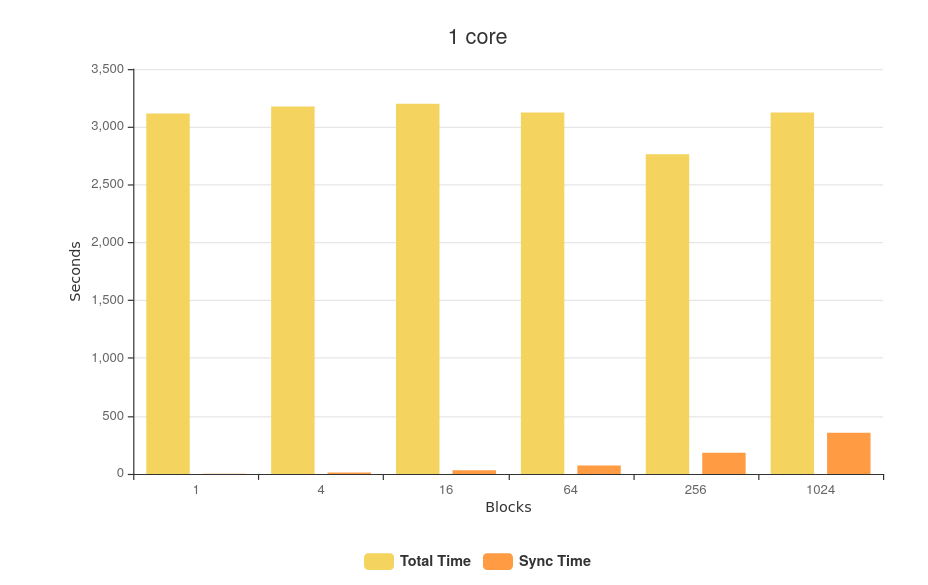
\includegraphics[width=0.6\linewidth, height=180pt]{block_result.png}
    \caption{Тестирование блочного подхода на одном ядре. По вертикальной оси - время в секундах: желтым цветом - общее время работы модели; оранжевым - время на синхронизации блоков. По горизонтальной оси - количество блоков в разбиении.}
    \label{fig:block_res}
\end{figure}
    
Был протестирован блочный подход на одном ядре CPU, т.е. последовательная версия модели.
Расчет проводился на сетке с размером 1525 x 1115 точек.
%Тестирование проводилось на процессоре Intel Xeon Silver 4214.
На рис. \ref{fig:block_res} показано время работы модели в зависимости от количества блоков, участвующих в разбиении области. Видно, что с увлечением количества блоков в разбиении (т.е. с уменьшением размера блока т.к. разбиение на блоки равномерное) общее время расчета модели увеличивается из-за затрат на копирование границ блоков на внерасчетные границы соседних блоков.
Когда размеры блоков становятся достаточно малыми, а именно когда разбиение начинает состоять из 256 блоков, происходит ускорение на 12\% по сравнению с неблочным подходом за счет эффективной работы с кэш памятью в блочном подходе.
И хоть общее время расчета продолжает далее увеличиваться с уменьшением размера блоков, при 1024 блоков в разбиении оно выравнивается со временем неблочного подхода.
Из всего этого можно сделать вывод, что, если выбирать малые размеры блоков, то эффективная работа с кэш памятью компенсирует затраты на копирование границ блоков при синхронизации.
Для рассмотренной акватории получилось, что оптимальный размер блока, получаемый
при разбиении области на 256 блоков, соответствует размеру 95 на 69 точек. Поскольку в вычислениях используются числа с плавающей запятой двойной точности (64 бита на одно число), то один такой блок занимает около 50 Кбайт в памяти.

\begin{figure}[!ht]
	\begin{minipage}{0.5\linewidth}
	\centering
	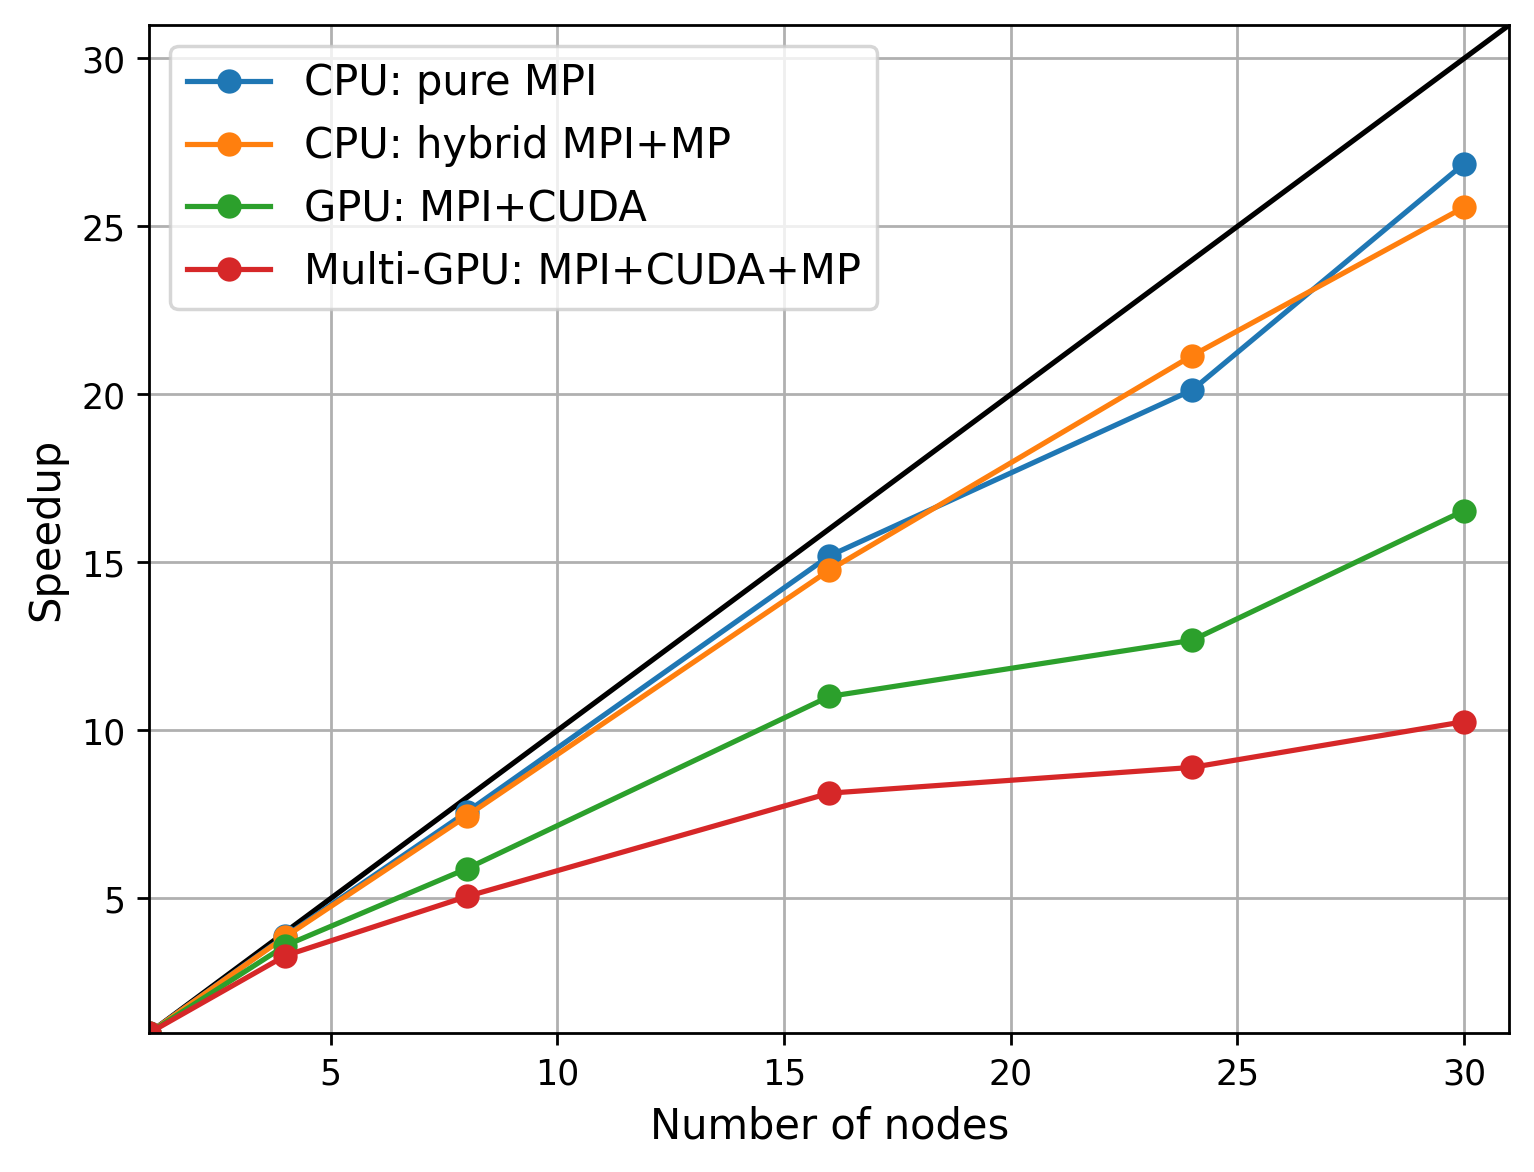
\includegraphics[width=\linewidth]{v3_3_6100x4460_pascal_speedup_multiGPU_V.png}
	\subcaption{Ускорение}
	\end{minipage}
	\begin{minipage}{0.5\linewidth}
	\centering
    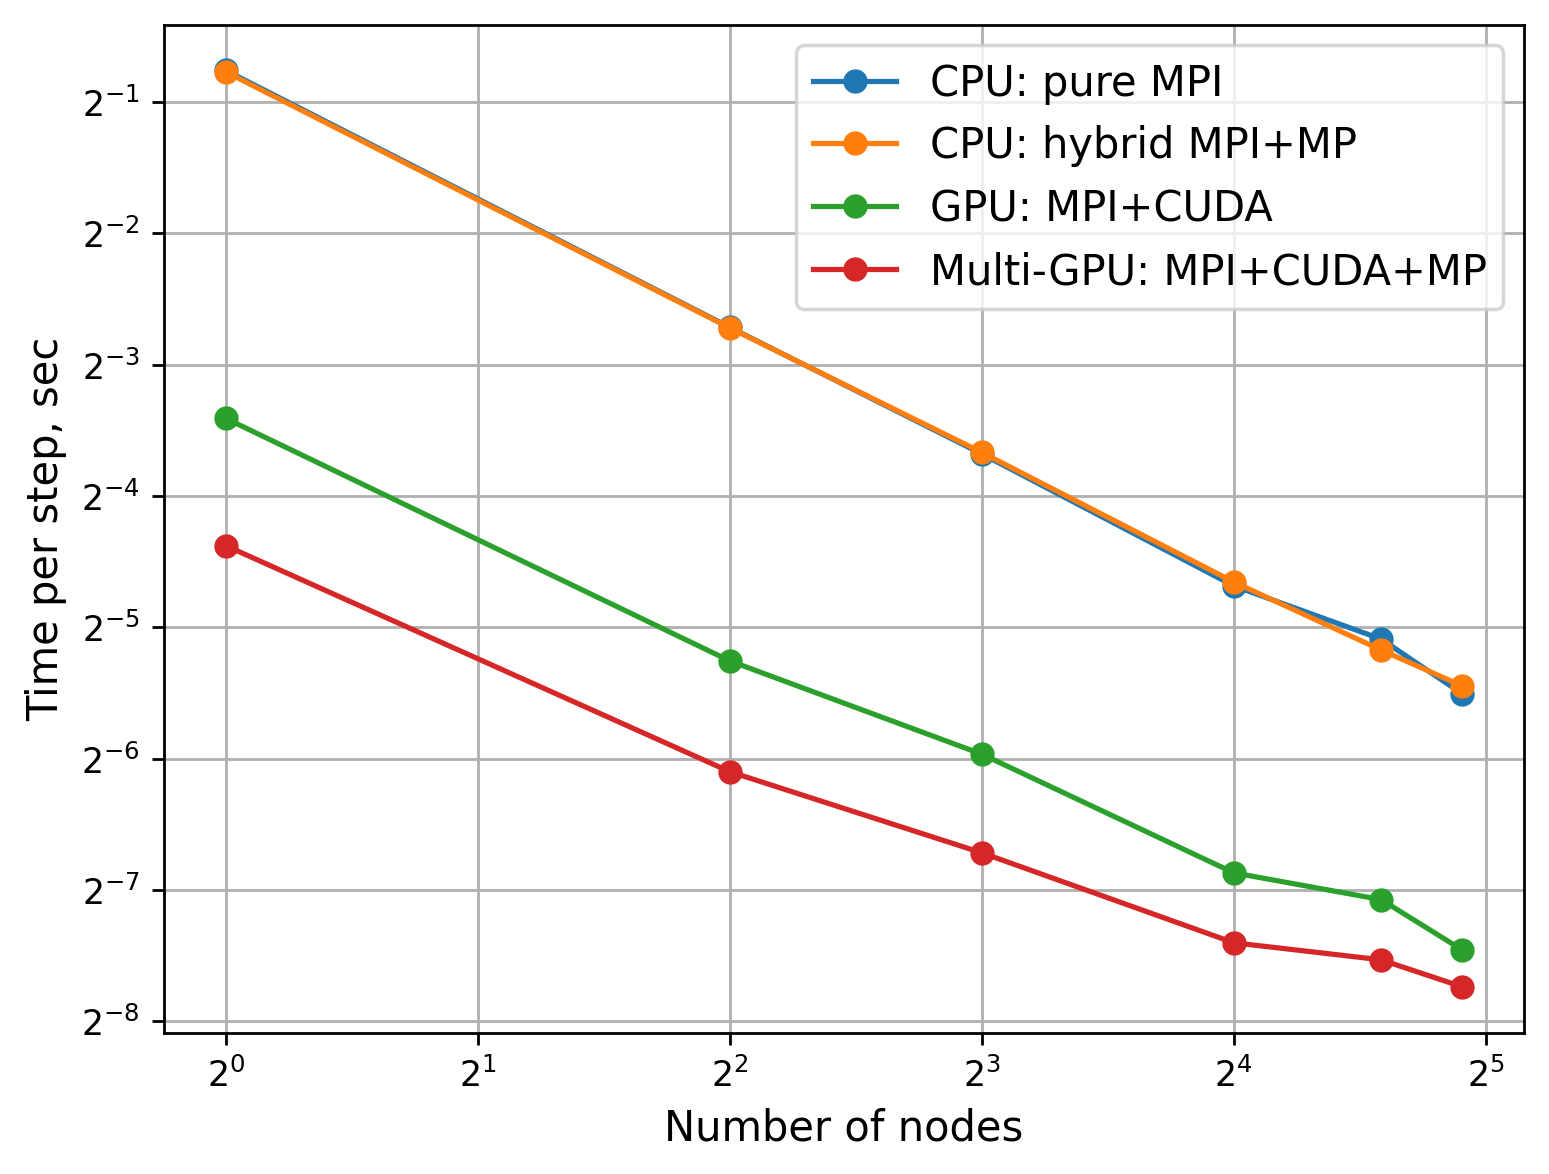
\includegraphics[width=\linewidth]{v3_3_6100x4460_pascal_time_multiGPU_V.png}
	\subcaption{Время одного шага модели (в логарифмической шкале)}
	\end{minipage}
	\vspace{3pt}
	\caption{Масштабирование производительности на разделе Pascal для размера сетки 6100 $\times$ 4460.}
	\label{fig:TheBox}
\end{figure}

Был проведён анализ эффективности и масштабируемости гибридных методов для расчётов мелкой воды с использованием GPU в сравнении с методами расчётов на CPU при размере сетки 6100 x 4460 точек (см. рис \ref{fig:TheBox}).
Представленные результаты на рисунке получены с использованием 30 узлов раздела Pascal суперкомпьютера Ломоносов-2. Чистый MPI подход и гибридные MPI-OpenMP подходы на CPU демонстрируют близкое к линейному (черная линия на рисунке) масштабирование до 30 узлов (всего 360 ядер).
Однако гибридный подход MPI-OpenMP не смог превзойти чистый MPI подход на этом суперкомпьютере. 
Шаблон MPI-OpenMP-CUDA с использованием нескольких GPU на вычислительном узле позволяет выполнять вычисления на 60 GPU с использованием 30 узлов и демонстрирует лучшую производительность благодаря эффективному использованию всех вычислительных ресурсов на узле.
Этот подход имеет в два раза лучшую производительность до 16 узлов, чем шаблон MPI-CUDA с одним GPU на узел, но затем разница в производительности уменьшается из-за небольшого размера подобласти на графический процессор.
Расчет на одном GPU превосходит любой шаблон вычислений на CPU примерно в 6.3 раза, как видно из графиков. 
Несмотря на то что масштабирование производительности на GPU хуже, чем на CPU, вычисления на GPU по-прежнему превосходят вычисления на CPU в 4.7 раза при использовании 60 GPU и 360 ядер CPU на 30 узлах.

\begin{figure}[!ht]
	\begin{minipage}{1\linewidth}
	\centering
	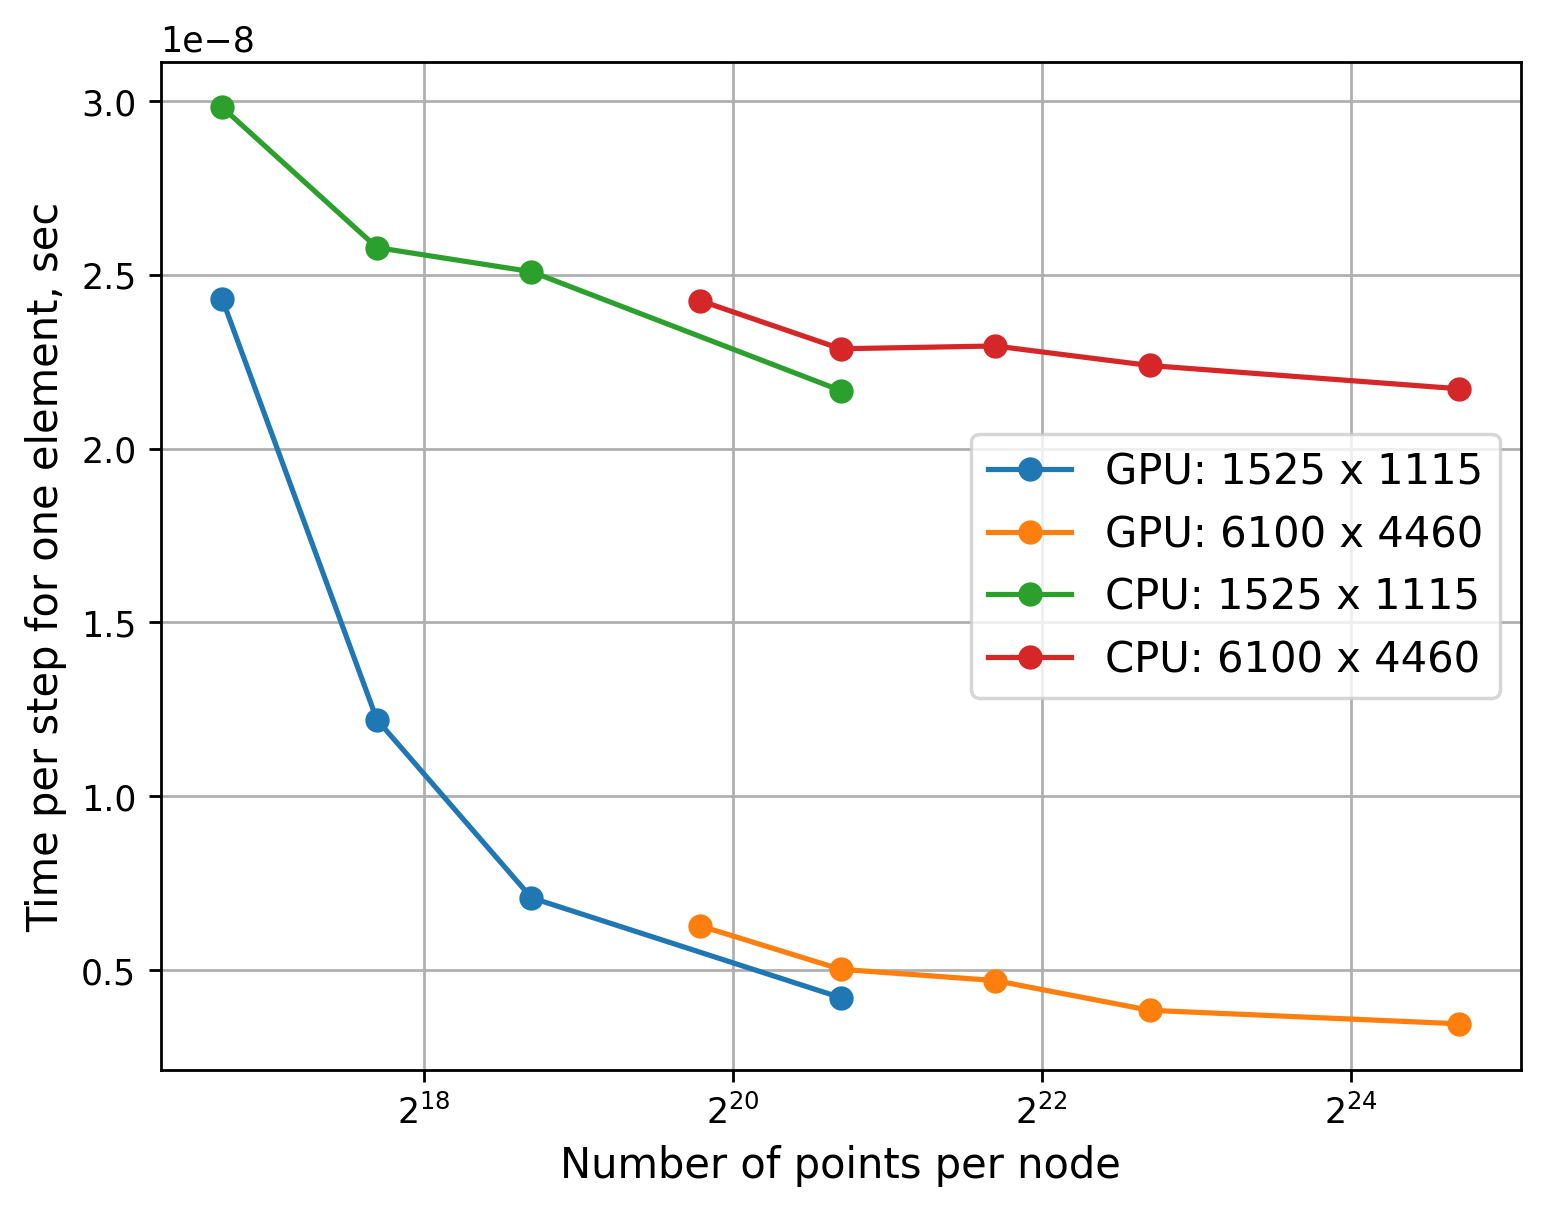
\includegraphics[width=0.5\linewidth]{v3_3_pascal_analysic_fix_1.png}
	\end{minipage}
	\vspace{3pt}
	\caption{Время на одну точку в вычислительной сетке (в логарифмической шкале). Был использован раздел Pascal суперкомпьютера Ломоносов-2.}
	\label{fig:TheBox_full}
\end{figure}

Мы также провели сравнение масштабирования производительности на CPU и GPU при размере сетки 1525 x 1115.
На рисунке \ref{fig:TheBox_full} показано время на одну точку в вычислительной сетке для расчетов на CPU и GPU с размерами сеток 1525 x 1115 и 6100 x 4460.
Из графика видно, что производительность на одну точку сетки на GPU резко снижается после $2^{19}$ точек на узел, в то время как производительность на CPU хорошо масштабируется до $2^{17}$ точек на узел. 
Следовательно, можно заключить, что GPU значительно чувствительнее к размеру сетки, в сравнении с CPU.
Это обусловлено двумя основными факторами.
Во-первых, накладные расходы на коммуникации, включая передачу данных между CPU и GPU, могут превысить время вычислений и стать узким местом производительности на GPU.
Во-вторых, небольшие подобласти приводят к более эффективному использованию кеш-памяти при вычислениях только на CPU, но не могут насытить вычисления и полностью скрыть задержки памяти на GPU.

Чтобы дополнительно исследовать масштабирование производительности на GPU, мы протестировали асинхронный шаблон вычисления MPI-OpenMP-CUDA, который перекрывает передачу данных с выполнением ядра по времени на GPU. Эксперименты на сетке размером 6100 × 4460 проводились на разделе Volta суперкомпьютера, включая Nvidia Tesla V100 на узлах.
На рисунке \ref{fig:asyncGPU_onenode} продемонстрированы показатели производительности при использовании разного числа блоков в блочной подходе на одном GPU. Видно, что асинхронный шаблон вычислений на GPU превосходит синхронный шаблон вычислений на 17\% благодаря параллельному выполнению ядра и передаче данных.
На рисунке \ref{fig:asyncGPU_onenode} показано производительность при использовании различного числа блоков в блочном подходе на одном GPU. Мы видим, что асинхронный шаблон вычислений на GPU превосходит синхронный на 17\% из-за перекрывания выполнения ядра и передачи данных по времени.
Рисунок \ref{fig:asyncGPU} показывает масштабирование производительности асинхронного шаблона вычислений на GPU при оптимальном числе блоков (8 блоков на GPU, как показано на рисунке \ref{fig:asyncGPU_onenode}) по сравнению с синхронным шаблоном вычислений на графических процессорах.
Этот эксперимент показывает, что асинхронный шаблон лучше масштабируется до 8 узлов и на 28\% быстрее на 8 графических процессорах по сравнению с синхронным шаблоном вычислений.
Кроме того, данный эксперимент показывает, что перекрывание выполнение ядра с передачей данных по времени на GPU компенсирует накладные расходы на копирование граничных значений блоков во время синхронизации в блочном подходе.
Однако это утверждение справедливо только для достаточно больших вычислительных областей.

\begin{figure}[!ht]
	\begin{minipage}{1\linewidth}
	\centering
	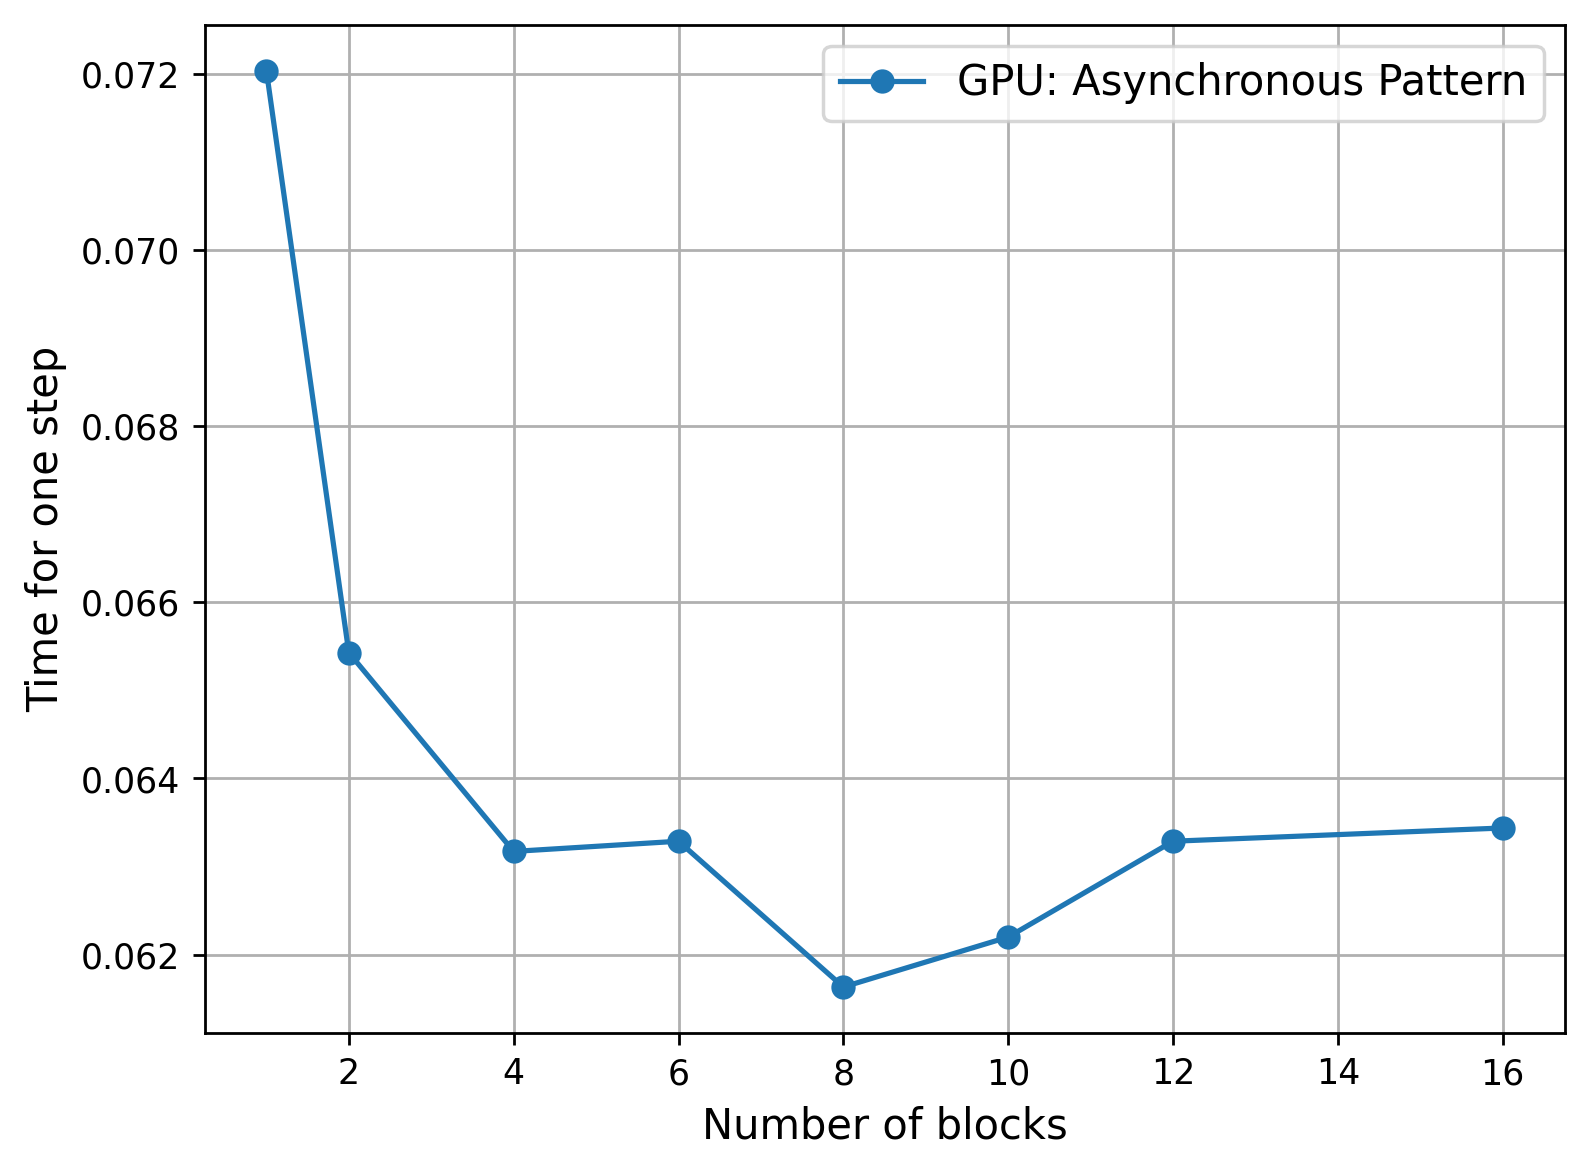
\includegraphics[width=0.5\linewidth]{v3_3_6100x4460_volta_async_blocks.png}
	\end{minipage}
	\vspace{3pt}
	\caption{Время на один шаг модели (в логарифмической шкале) на одном GPU V100 для сетки размером 6100 $\times$ 4460.}
	\label{fig:asyncGPU_onenode}
\end{figure}

\begin{figure}[!ht]
	\begin{minipage}{0.5\linewidth}
	\centering
	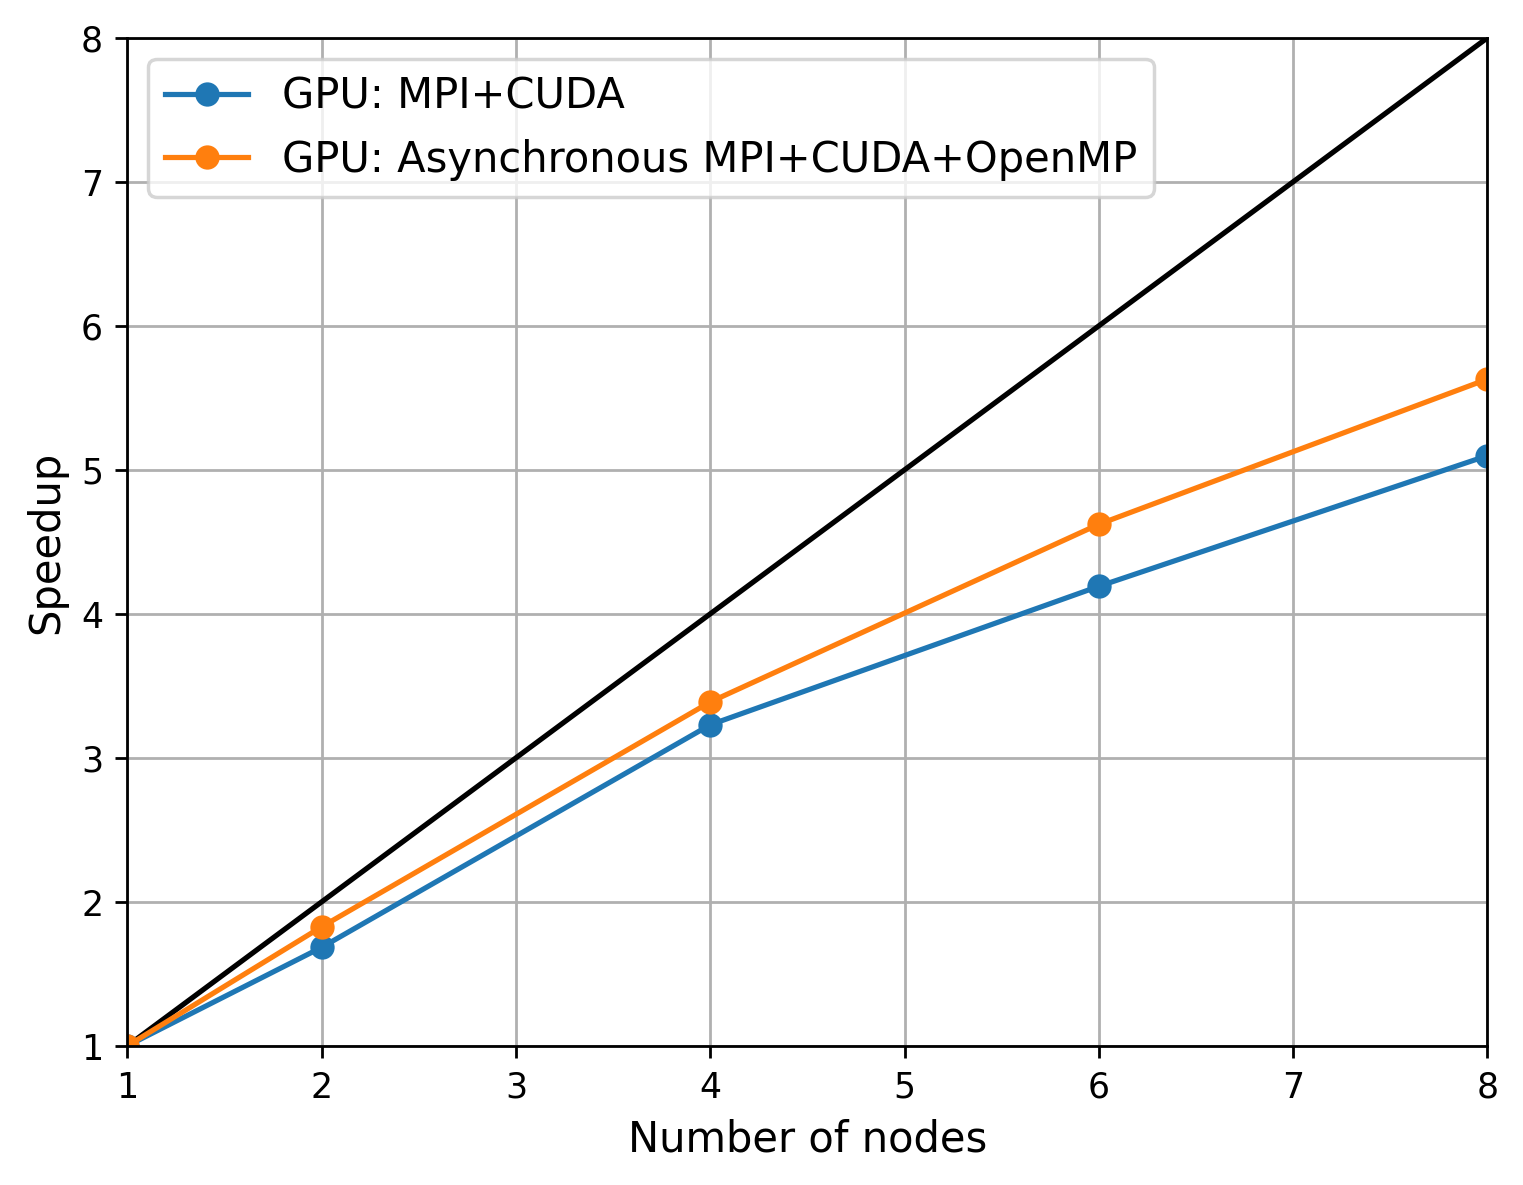
\includegraphics[width=1\linewidth]{v3_3_volta_speedup_renamed.png}
	\subcaption{Ускорение}
	\end{minipage}
	\begin{minipage}{0.5\linewidth}
	\centering
	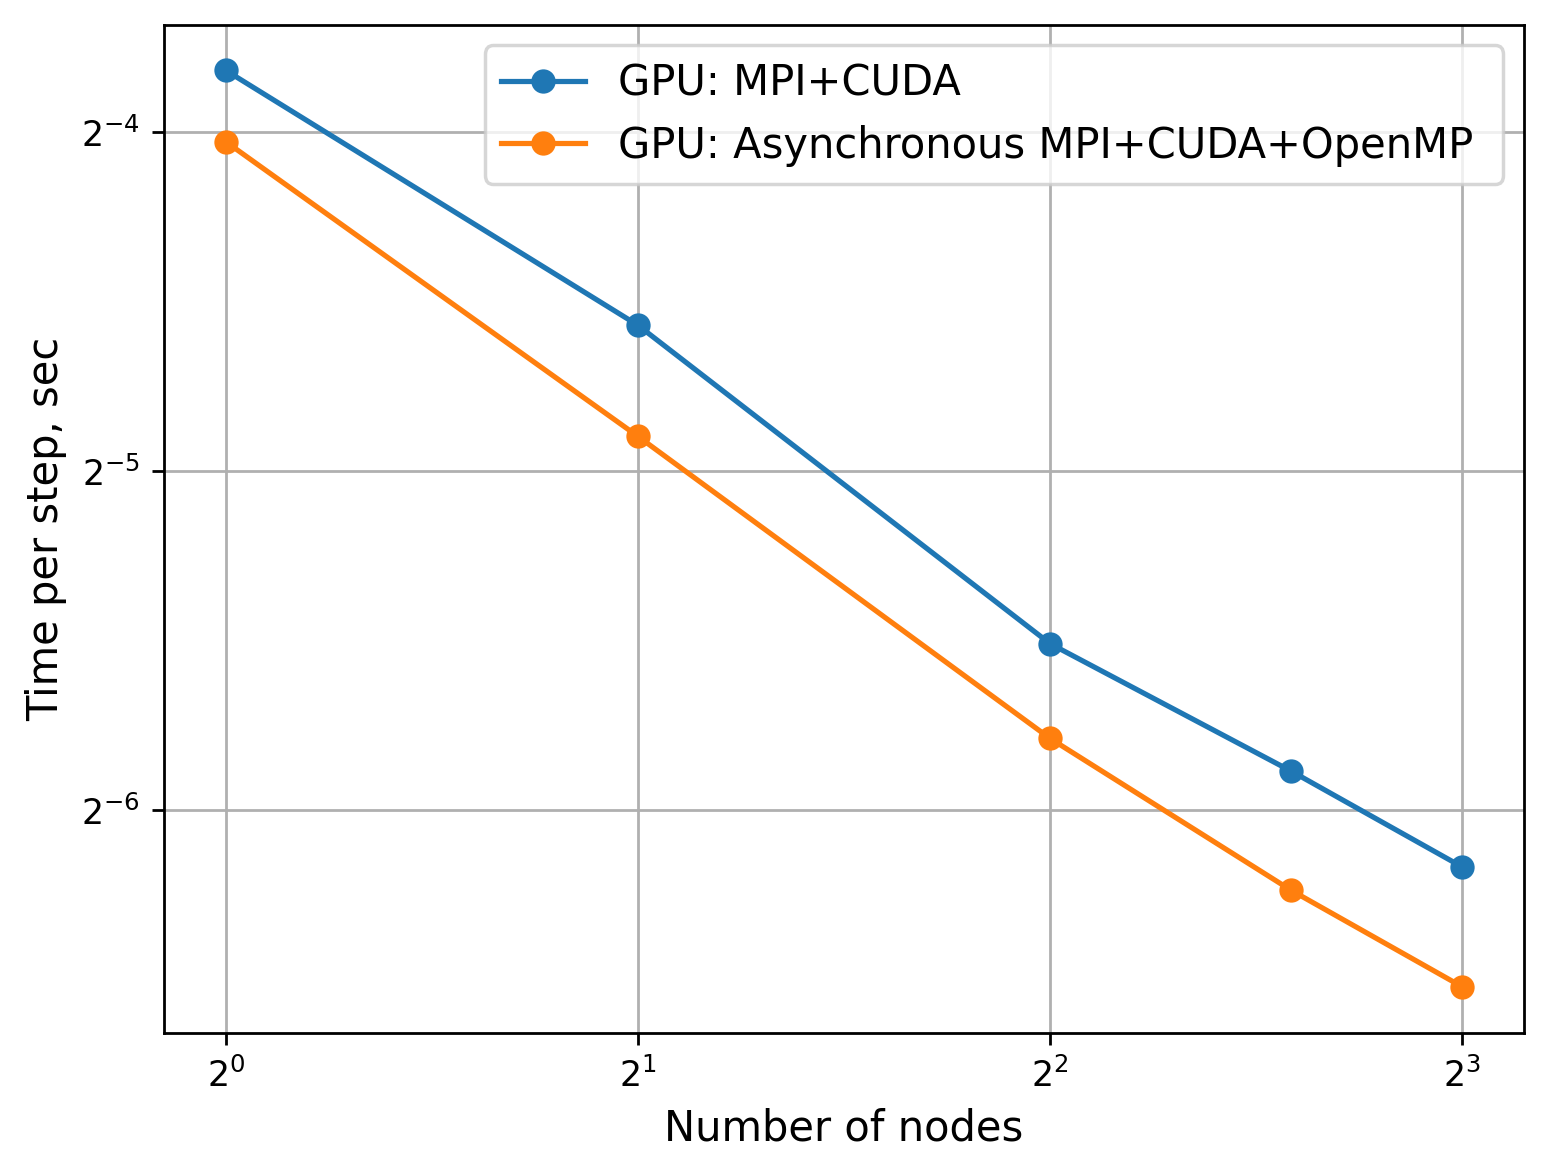
\includegraphics[width=1\linewidth]{v3_3_volta_time_renamed.png}
	\subcaption{Время на один шаг модели (в логарифмической шкале)}
	\end{minipage}
	\vspace{3pt}
	\caption{Масштабирование производительности на GPU V100 для размера сетки 6100 $\times$ 4460.}
	\label{fig:asyncGPU}
\end{figure}

\subsection{Тестирование Азовского Моря}\label{sec:ch3/sec1/sub2}

Азовское море представляет собой подходящий регион для тестирования двумерных численных моделей мелкой воды, так как его гидродинамические процессы могут быть точно и эффективно описаны такими моделями в связи с его относительной мелководностью \cite{Azov}.
Кроме того, вычислительная область Азовского моря обладает значительным количеством наземных точек, что делает целесообразным применение техники балансировки загрузки.
На рисунке \ref{fig:LB} показано, что более половины блоков полностью находятся на суше при делении области на блоки небольшого размера.
Вторая серия экспериментов была проведена в Азовском море с целью оценить масштабирование производительности модели мелкой воды с неравномерной нагрузкой на процессоры и продемонстрировать преимущества использования метода балансировки нагрузки для вычислений на CPU и GPU.
Мы провели тестирование моделей с разным пространственным разрешением: 250 метров (сетка размером 1525 $\times$ 1115) и 62.5 метров (сетка размером 6088 $\times$ 4448). Моделирование было проведено в течение одних суток модельного времени, с общим числом шагов 86400.  

%Метрика $LB$ отвечает за балансировку разделения в терминах нагрузки на процессоры и определяется следующим образом. Предположим, что разделение происходит на $k$ поддоменов для $p$ процессоров, тогда $LB$ определяется как уравнение 5, где $\max_{1 \leq i \leq k} W_i$ - это максимальная нагрузка $i$-го поддомена, а $\sum_{i=1}^k W_i$ - это общая нагрузка всей вычислительной области.

Расчет нагрузки выполняется по-разному для вычислений на CPU и GPU.
Для CPU метрика загруженности подобласти представляет собой сумму "влажных" точек в подобласти, как было показано в разделе \ref{sec:ch2/sec3/lb}, см. уравнение \ref{eq:LB}.
Однако для графических процессоров нагрузка подобласти представляет сумму всех точек (как "сухих", так и "влажных").
Из-за расходящихся путей выполнения, производительность на GPU не уменьшается с увеличением доли "влажных" точек, в отличие от CPU \cite{kirk10}.
Поэтому для вычислений на GPU мы равномерно распределяем блоки из блочного разбиения между GPU, исключая полностью блоки, которые попадают на сушу.

Как упоминалось ранее, блочное разбиение разделяет область на небольшие блоки и распределяет их среди доступных процессоров.
С одной стороны, использование небольшого числа блоков в разделении приводит к высокому значению метрики $LB$ (см. уравнение \ref{eq:LB}) и несбалансированным подобластям процессоров.
С другой стороны, использование большого числа блоков в разделении приводит к высоким накладным расходам при копировании граничных значений блоков во время синхронизации процессоров, что особенно важно для вычислений на GPU, поскольку мы должны передавать данные между CPU и GPU для каждого блока.
Поэтому количество блоков $k$ в разделении выбирается адаптивно для распределения среди $p$ процессоров в соответствии с следующим критерием:

\begin{equation} \label{eq:LB_GPU} 
k(p) = \min_{n=0,1,...} \{ 4^n ~|~ LB(4^{n}, p) - LB(4^{n+1}, p) < 0.15 \}
\end{equation}


\begin{table} [htbp]
\centering
%\begin{threeparttable}% выравнивание подписи по границам таблицы
\caption{Метрики LB для Азовского моря с разрешением 250 метров}\label{tab:CPULB}
	\begin{tabular}{cccc}
	$p$ & $LB$ для 256 блоков & $LB$ для 1024 блоков & $LB$ для 4096 блоков \\
    \hline
	48    &  1.371   &  \textbf{1.045}  &  1.012 \\
    96    &  1.802   &  \textbf{1.154}  &  1.022 \\
	192   &    -     &  1.385  &  \textbf{1.070} \\
	\hline
	\end{tabular}
%\end{threeparttable}
\end{table}

Таблица \ref{tab:CPULB} демонстрирует оптимальное количество блоков для вычислений на разном количестве процессоров согласно описанному критерию; оптимальное количество блоков выделено в таблице.

Мы провели тестирование модели Азовского моря на разделе Pascal суперкомпьютера Ломоносов-2.
На рисунке \ref{fig:AzovSea} показана зависимость производительности модели с балансировкой нагрузки по сравнению с моделью без балансировки нагрузки на CPU при размере сетки 1525 $\times$ 1115 и на GPU при размере сетки 6088 $\times$ 4448.
Мы рассматривали только чистый MPI подход на CPU и сравнивали асинхронный шаблон вычислений MPI-OpenMP-CUDA с синхронным шаблоном вычислений MPI-CUDA на GPU.
На одном узле модель вычислялась без балансировки нагрузки.
Мы использовали оптимальное количество блоков в соответствии с критерием \ref{eq:LB_GPU}.
Для проведения вычислений на CPU, было выбрано оптимальное количество блоков в разбиении согласно Таблице \ref{tab:CPULB}; для проведения вычислений на GPU использовались 64 блока для 4 узлов и 256 блоков для 16 узлов.

Как видно из Рисунка \ref{fig:AzovSea}, метод балансирования нагрузки оказывает значительное влияние на производительность модели на CPU – схема с балансированием нагрузки демонстрирует рост на 30\% по сравнению со схемой без балансирования при использовании 16 узлов, при этом демонстрируя сверхлинейное масштабирование благодаря эффективности кэш-памяти за счет использования блоков малого размера.
При работе на GPU можно отметить, что асинхронный подход с балансировкой нагрузки увеличивает производительность на 30\% и 18\% соответственно по сравнению с синхронным и асинхронным шаблонами вычислений без балансирования нагрузки при использовании 16 узлов.
Однако, несмотря на увеличенное разрешение сетки, производительность на GPU масштабируется хуже по сравнению с CPU. Как было отмечено ранее, GPU более чувствительны к размерам задачи по сравнению с CPU (см. рис. \ref{fig:TheBox_full}).
Это особенно важно в данном контексте, поскольку с увеличением числа узлов число точек на GPU значительно снижается из-за наличия наземных точек в вычислительной области.

\begin{figure}[!ht]
	\begin{minipage}{0.5\linewidth}
	\centering
	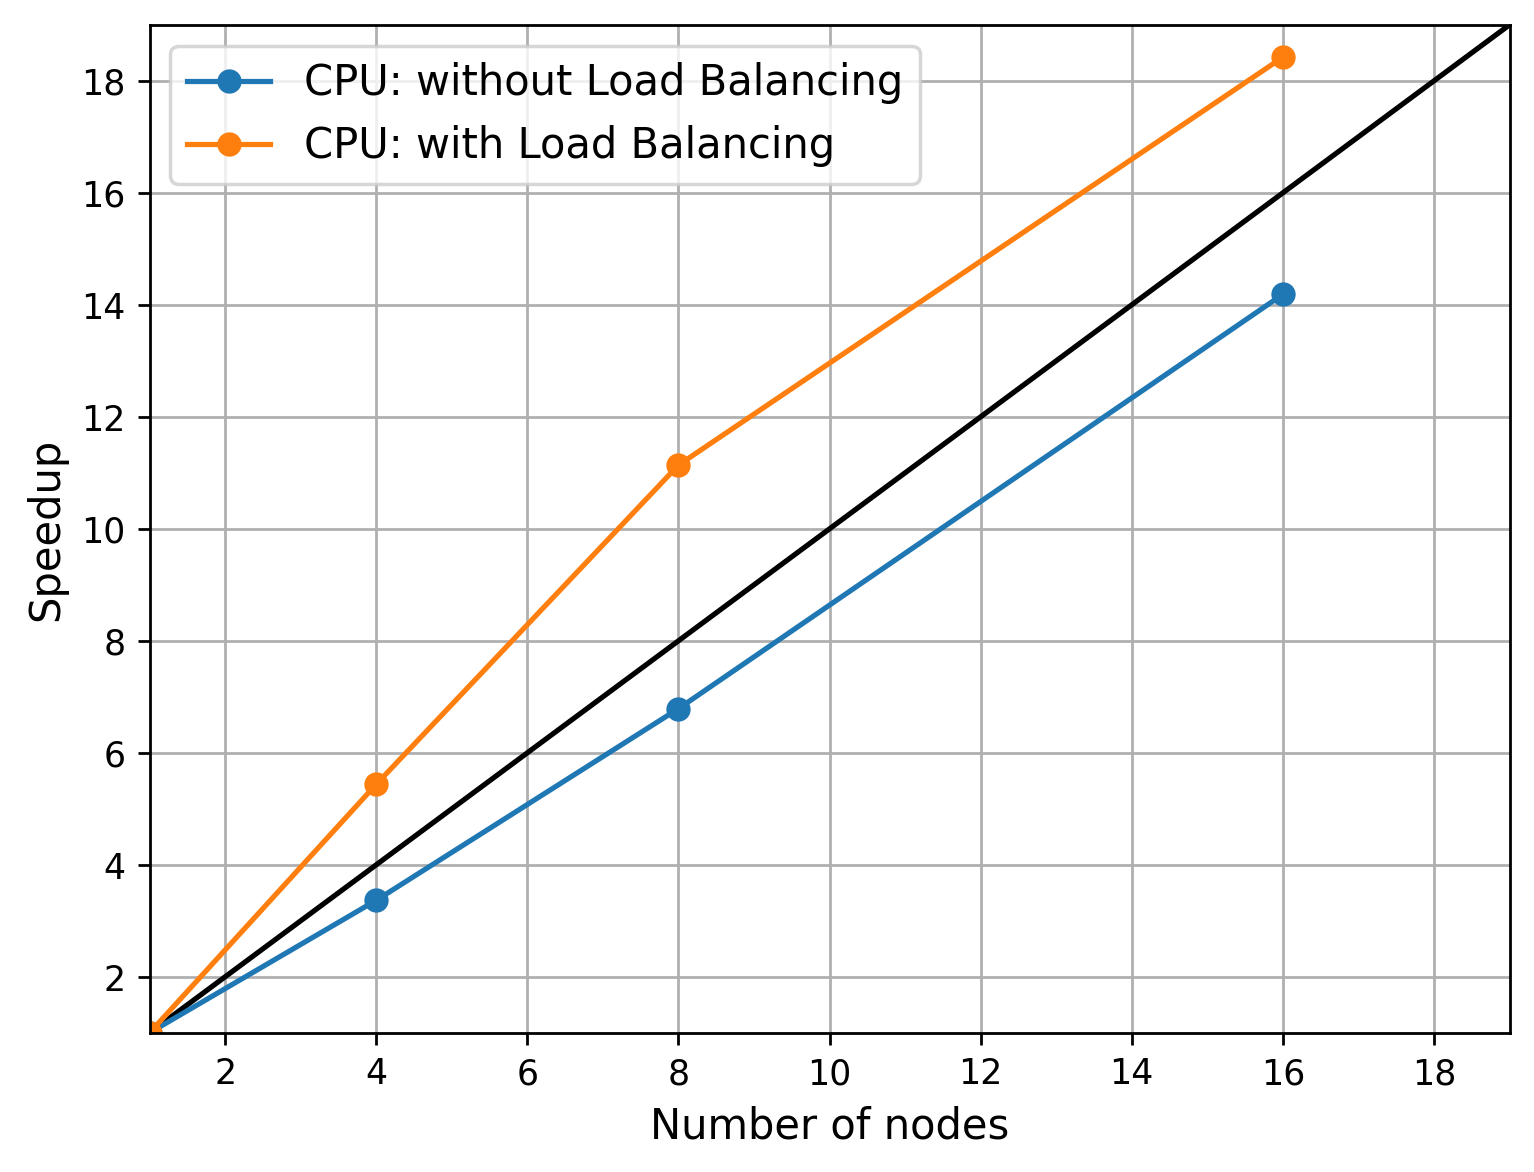
\includegraphics[width=\linewidth]{v3_3_AS250m_pascal_CPU_LB_speedup.png}
	\subcaption{Ускорении CPU версии модели с пространственным разрешением 250 м}
	\end{minipage}
	\begin{minipage}{0.5\linewidth}
	\centering
    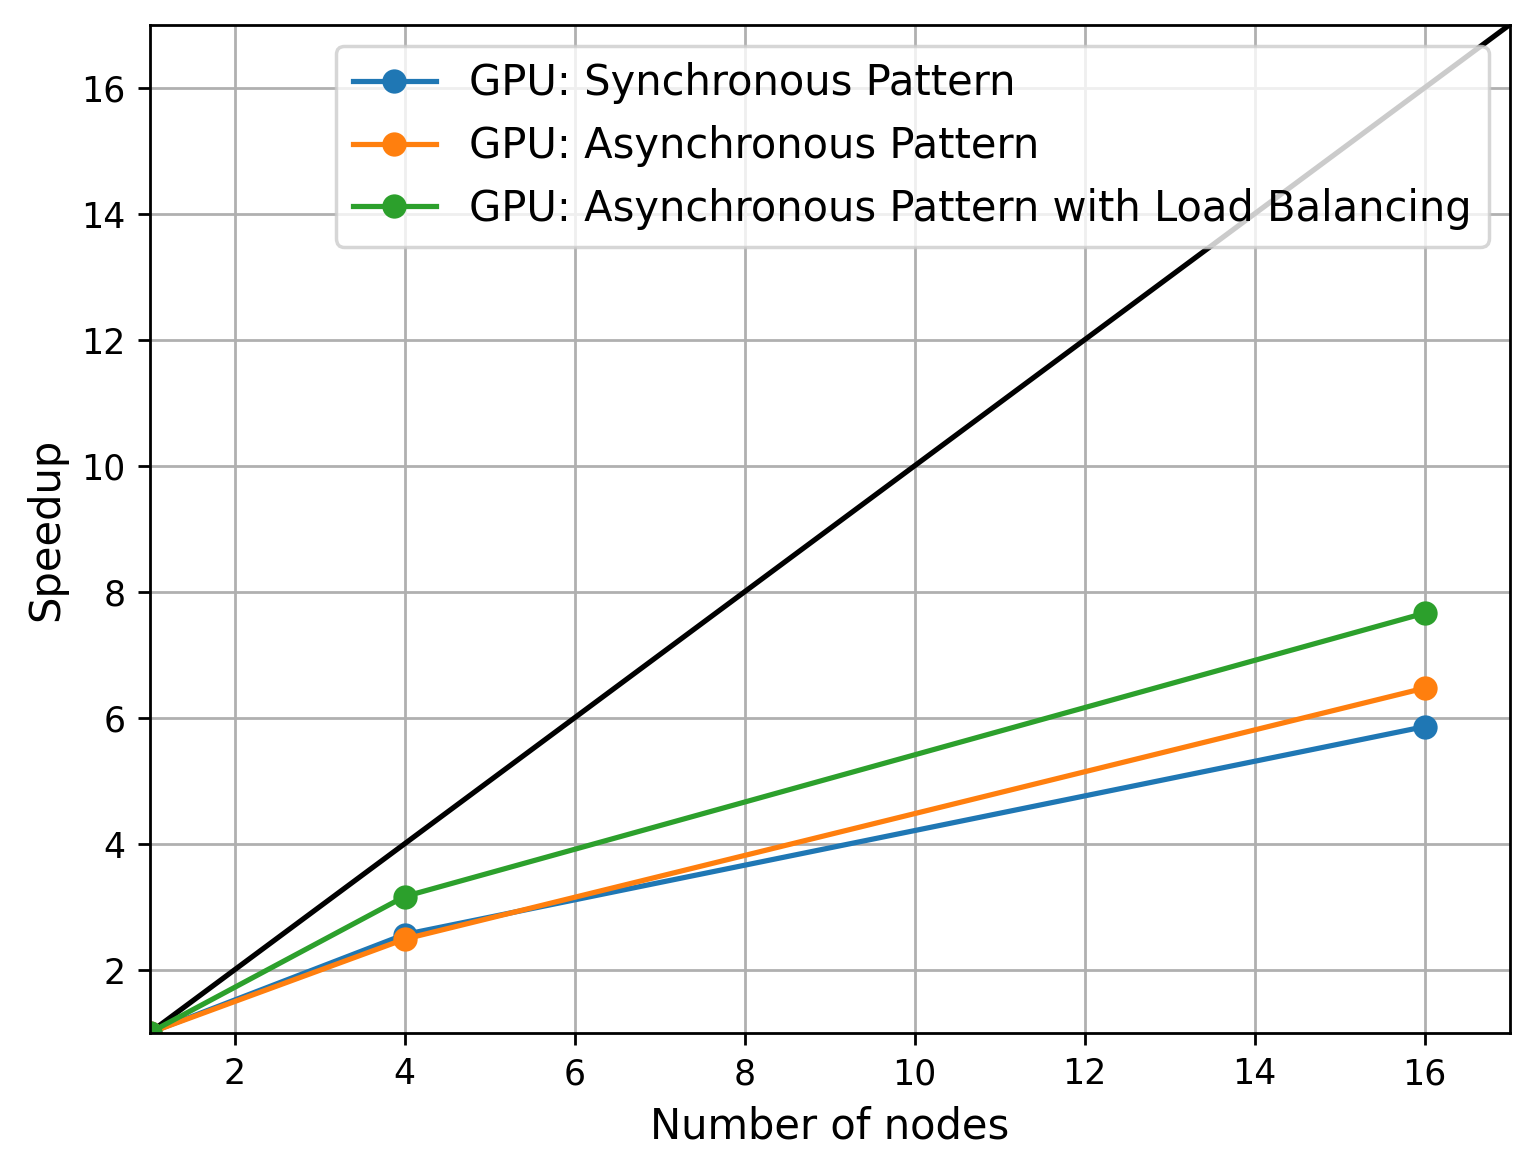
\includegraphics[width=\linewidth]{v3_3_AS62_5m_pascal_GPU_LB_speedup_cut.png}
	\subcaption{Ускорение GPU версии с пространственным разрешением 62.5 метров}
	\end{minipage}
	\vspace{3pt}
	\caption{Масштабирование производительности для акватории Азовского моря. Был использован раздел Pascal суперкомпьютера Ломоносов-2.}
	\label{fig:AzovSea}
\end{figure}

\section{Тестирование сигма-модели общей циркуляции океана INMOM для акватории Азовского моря}\label{sec:inmsom/ch3/sec1}

В этом разделе приводятся результаты по тестированию метода нагрузки балансировки вычислений  с использованием кривых Гильберта уже применительно к полной трехмерной сигма-модели циркуляции океана INMOM, которая была описана в главе \ref{ch:inmsom/ch1} и разделе \ref{sec:inmsom/ch2/sec1}.
	
Тестирование модели проводилось на кластере ИВМ РАН. Кластер состоит из головного узла, вспомогательного узла и вычислительных узлов,
объеденных в разные группы. Тестирование проводилось преимущественно на группе вычислительных узлов x8core, состоящих из двух 8-ядерных процессоров Intel Xeon E5-2665@2.40ГГц и с 64 Гб оперативной памяти.
%	Характеристики вычислительных узлов в группе x8core:
%	\begin{itemize}
%	\setlength\itemsep{0.0em}
%	\item Compute Node Arbyte Alkazar+ R2Q50.
%	\item 16 ядер (два 8-ядерных процессора Intel Xeon E5-2665@2.40ГГц).
%	\item Оперативная память: 64 Гб.
%	\end{itemize}
	На кластере установлены последние версии компиляторов Intel Fortran (ifort) и библиотек MPI, с помощью которых собиралась и тестировалась модель.
	
Метод балансировки нагрузки вычислений рассматривался на следующих сетках блоков:
	по 8 блоков на ядро для 128 ядер и по 4 блока на ядро для всех остальных. 
	Тестирование проводилось для акватории Азовского моря, см. \ref{sec:ch3/sec1/sub2}. Шаг по времени был выбран равным 30 секундам.
	
%	\begin{tabular}{|l|l|l|l|l|l|l|}
%    \hline
%    Cores    & 1 & 4 & 16 & 64 & 128 & 256 \\ 
%    \hline
%    Uniform  & 1 & 4 & 16 & 64 & 128 & 256 \\ 
%    \hline
%    Hilbert  & 1 & 4 & 16 & 64 & 128 & 256 \\ 
%    \hline
%    METIS    & 1 & 4 & 16 & 64 & 128 & 256 \\ 
%    \hline
%    \end{tabular}
%    }
%    \end{subtable}
%    \end{table}
	
	На рис. \ref{fig:inmom_hilbert1} и рис. \ref{fig:inmom_hilbert2} показано ускорение параллельной версии модели INMOM с методом балансировки, использующим кривые Гильберта, в сравнении с равномерным разбиением без балансировки и в сравнении с разбиением, полученным с помощью библиотеки METIS.      
    %Ускорение считалось по формуле (\ref{eq:speedup}),
    %где в качестве $T_{init}$ было взято время работы параллельной версии модели на 4 ядрах без балансировки нагрузки вычислений, на рис. \ref{fig:timemodelsteps} показано $T_{init}$ для различных блоков модели. 
Время работы разных блоков параллельной сигма-модели океана INMOM на 4 ядрах без балансировки нагрузки вычислений показано на рис. \ref{fig:timemodelsteps}.
Из графиков видно, что методы балансировки нагрузки вычислений дают 
    сверхлинейное ускорение для расчетов температуры и солености %(шаг 9 в модели, см. главу 4)
    и для
    расчета переноса и диффузии компонентов скорости. % (шаг 10 в модели, см. главу 4). 
    Это связано с тем, что при увеличении числа ядер, 
    большая часть блоков, попадающих полностью на сушу, выпадает из рассмотрения. % (см. таблицу 2).
    Более того, размер каждого блока становится мал и работа с кэш памятью становится наиболее эффективной.
    Исследования масштабируемости показали, что самым узким местом при распараллеливании модели океана является баротропная адаптация. % (шаг 16 в модели, см. главу 4).
    Это связано с тем, что
    на этой стадии решается линейная система алгебраических уравнений.
    Как уже было более подробно описано в \ref{sec:inmsom/ch2/sec1}, в качестве основного
    решателя был выбран
    метод GMRES с предобуславливателем ASM из библиотеки PETSc.
    Хоть и для этой стадии модели было получено самое низкое ускорение - 
    все равно видна эффективность метода балансировки нагрузки по сравнению с равномерным
    разбиением без балансировки.
    Для общего расчетного времени модели метод балансировки нагрузки дает почти линейное ускорение и по сравнению с равномерным разбиением без балансировки нагрузки ускорение больше в $\sim 1.7$ раза.
	Из графиков и таблицы \ref{tab:LB} видно, что метод балансировки нагрузки с использованием кривой Гильберта строит разбиения не хуже чем METIS.
	Для 128 и 256 ядер видно даже преимущество в ускорении, полученном с помощью
	этого метода, в сравнении с METIS.
	Похожие результаты были получены и при сравнении методов балансировки нагрузки
	применительно к уравнениям мелкой воды, разрешаемых по явной схеме по времени. % (см. главу 7.2). 
    В общем можно сделать вывод, что метод балансировки нагрузки вычислений с 
    использованием кривой Гильберта - это хорошая альтернатива библиотеке METIS.
    
	\begin{figure}[htb!]
    \begin{minipage}[h]{0.48\linewidth}
    \center{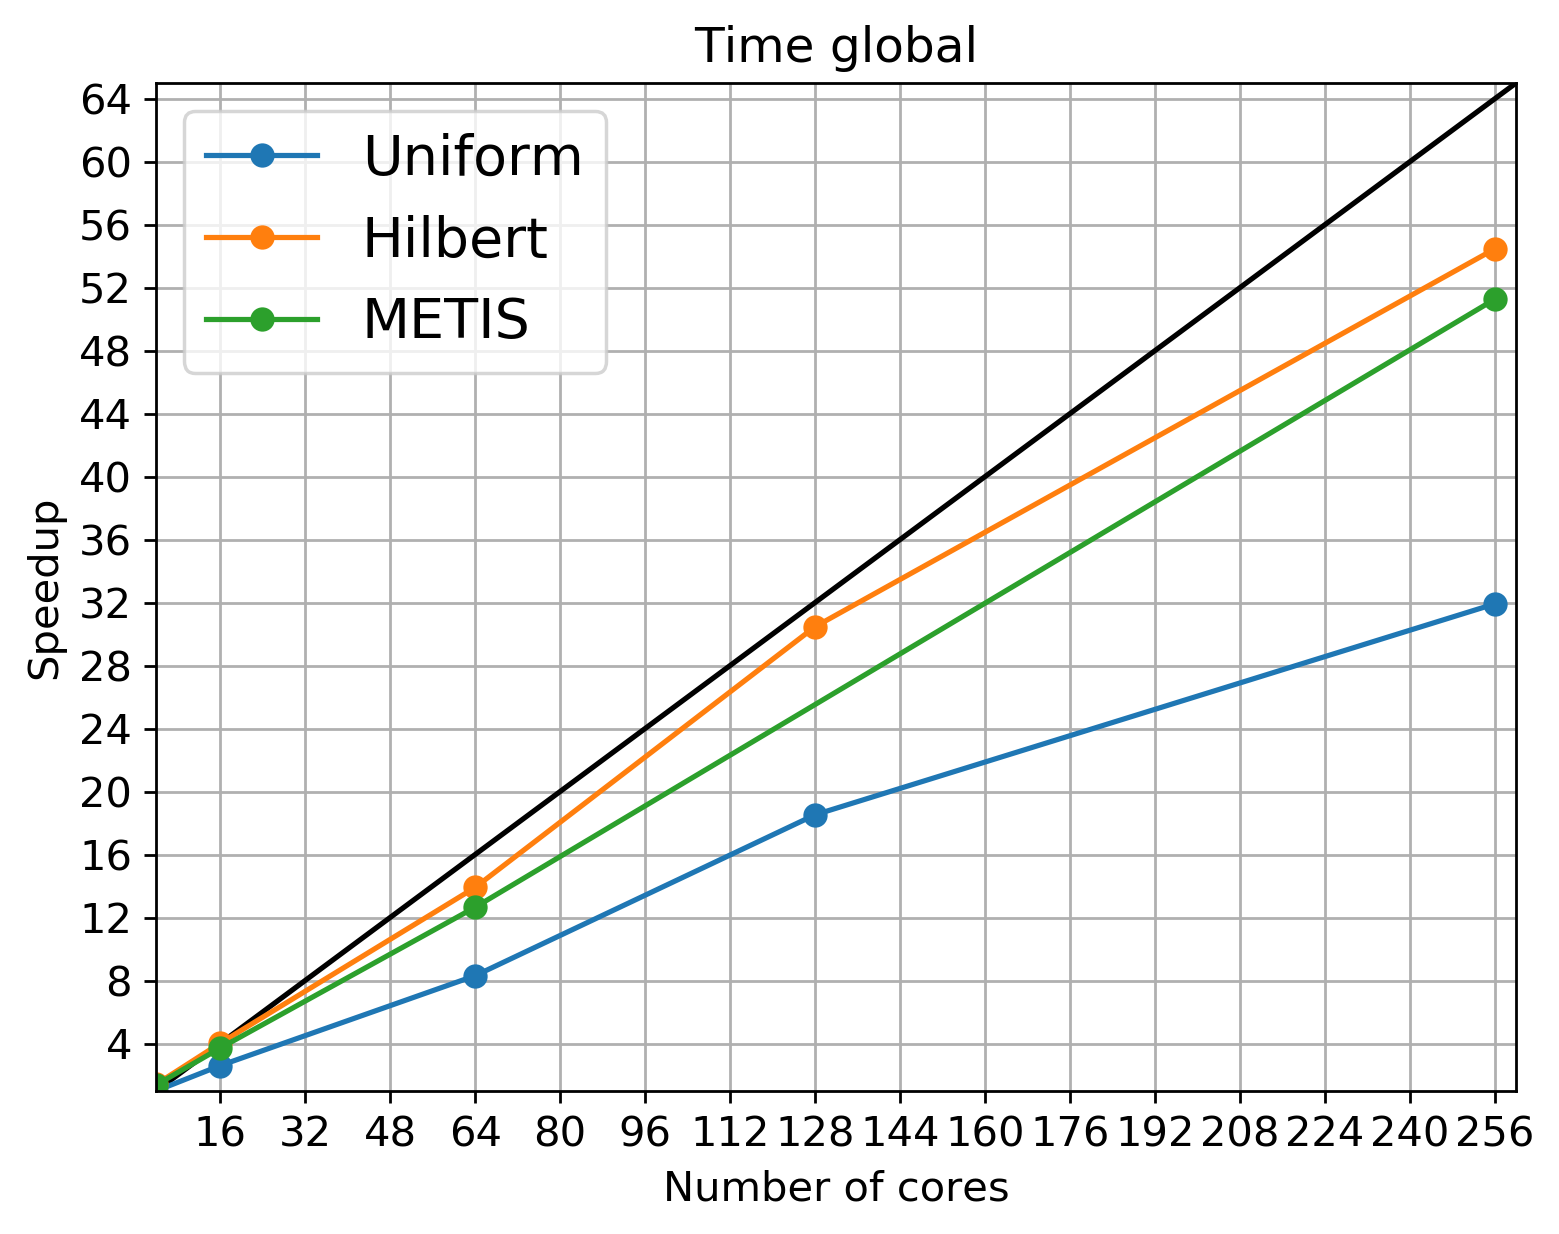
\includegraphics[width=1.0\linewidth]{plot4_upd_global.png}}
    \end{minipage}
    \hfill
    \begin{minipage}[h]{0.48\linewidth}
    \center{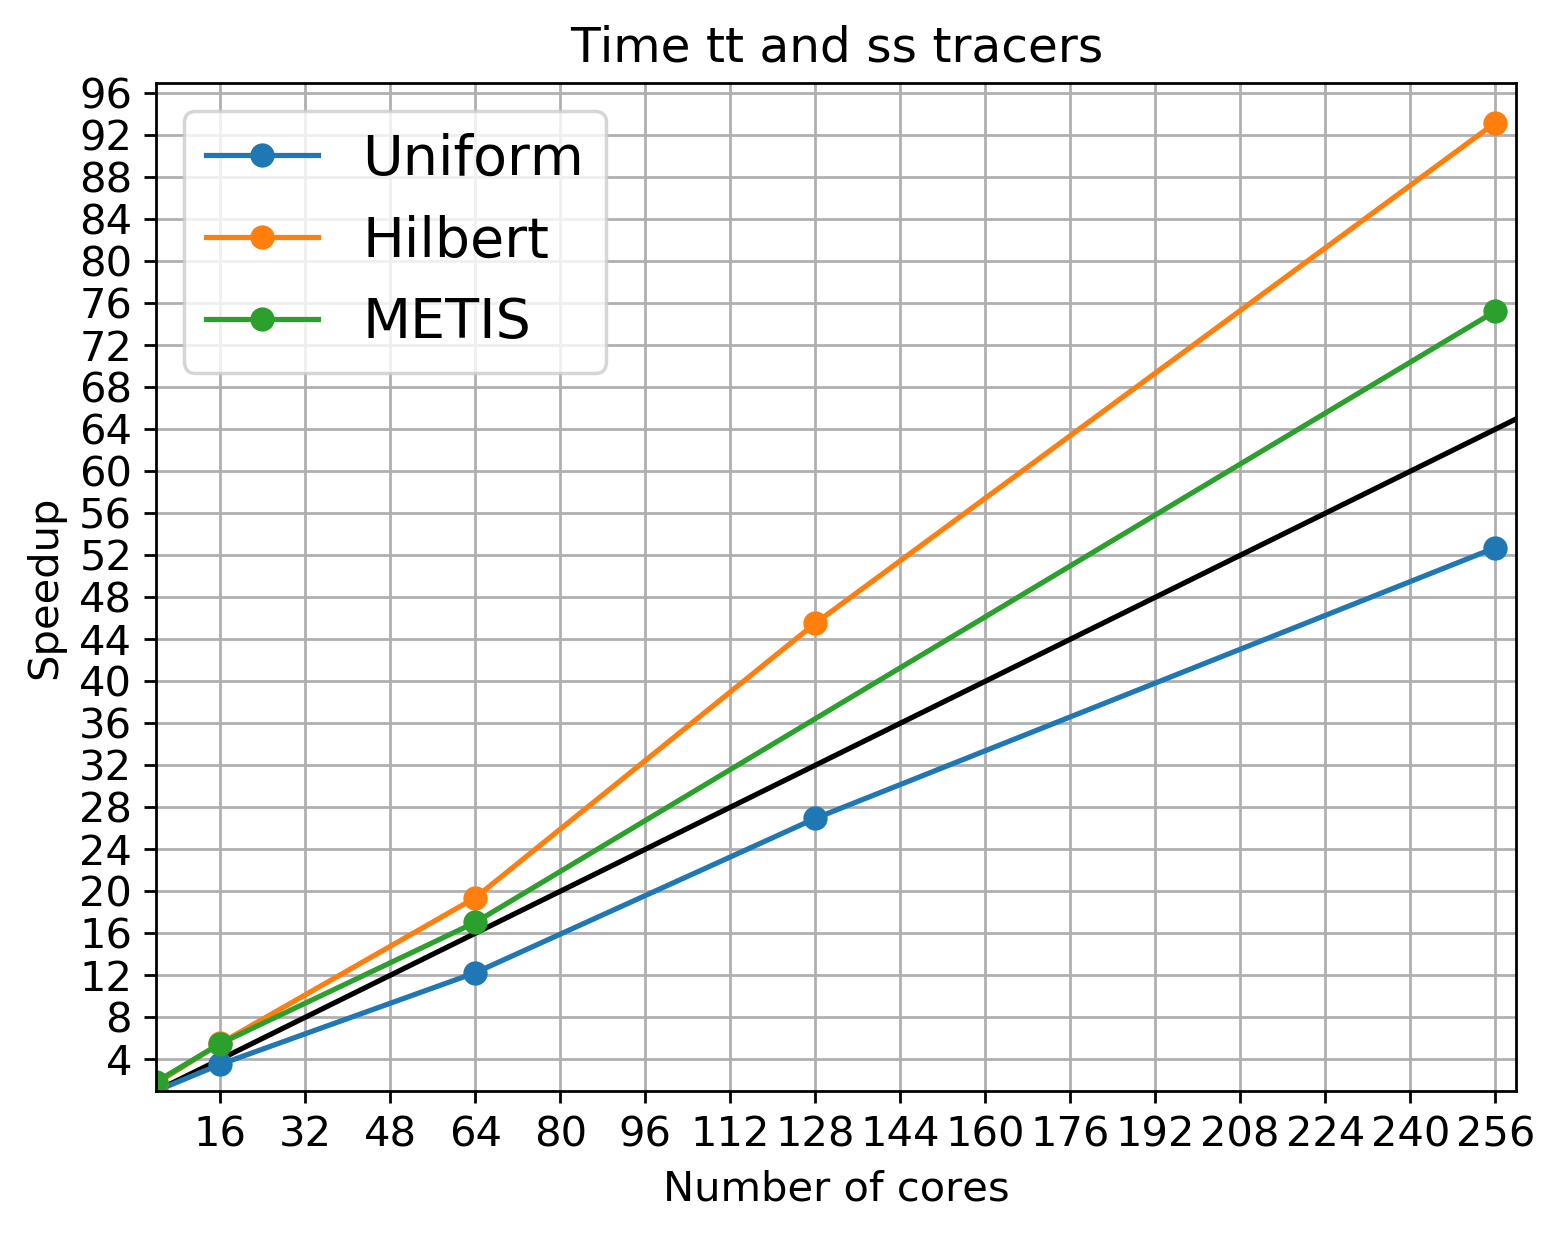
\includegraphics[width=1.0\linewidth]{plot4_upd_tt_ss.png}}
    \end{minipage}
    \caption{Модель океана INMOM. Ускорение метода разбиения с использованием кривых Гильберта в сравнении с равномерным разбиением и с METIS. 1) Общее время работы модели. 2) Расчет температуры и солености. 
    Чёрная линия соответствует линейному ускорению.}
    \label{fig:inmom_hilbert1}
    \end{figure}
    
     \begin{figure}[htb!]
    \begin{minipage}[h]{0.48\linewidth}
    \center{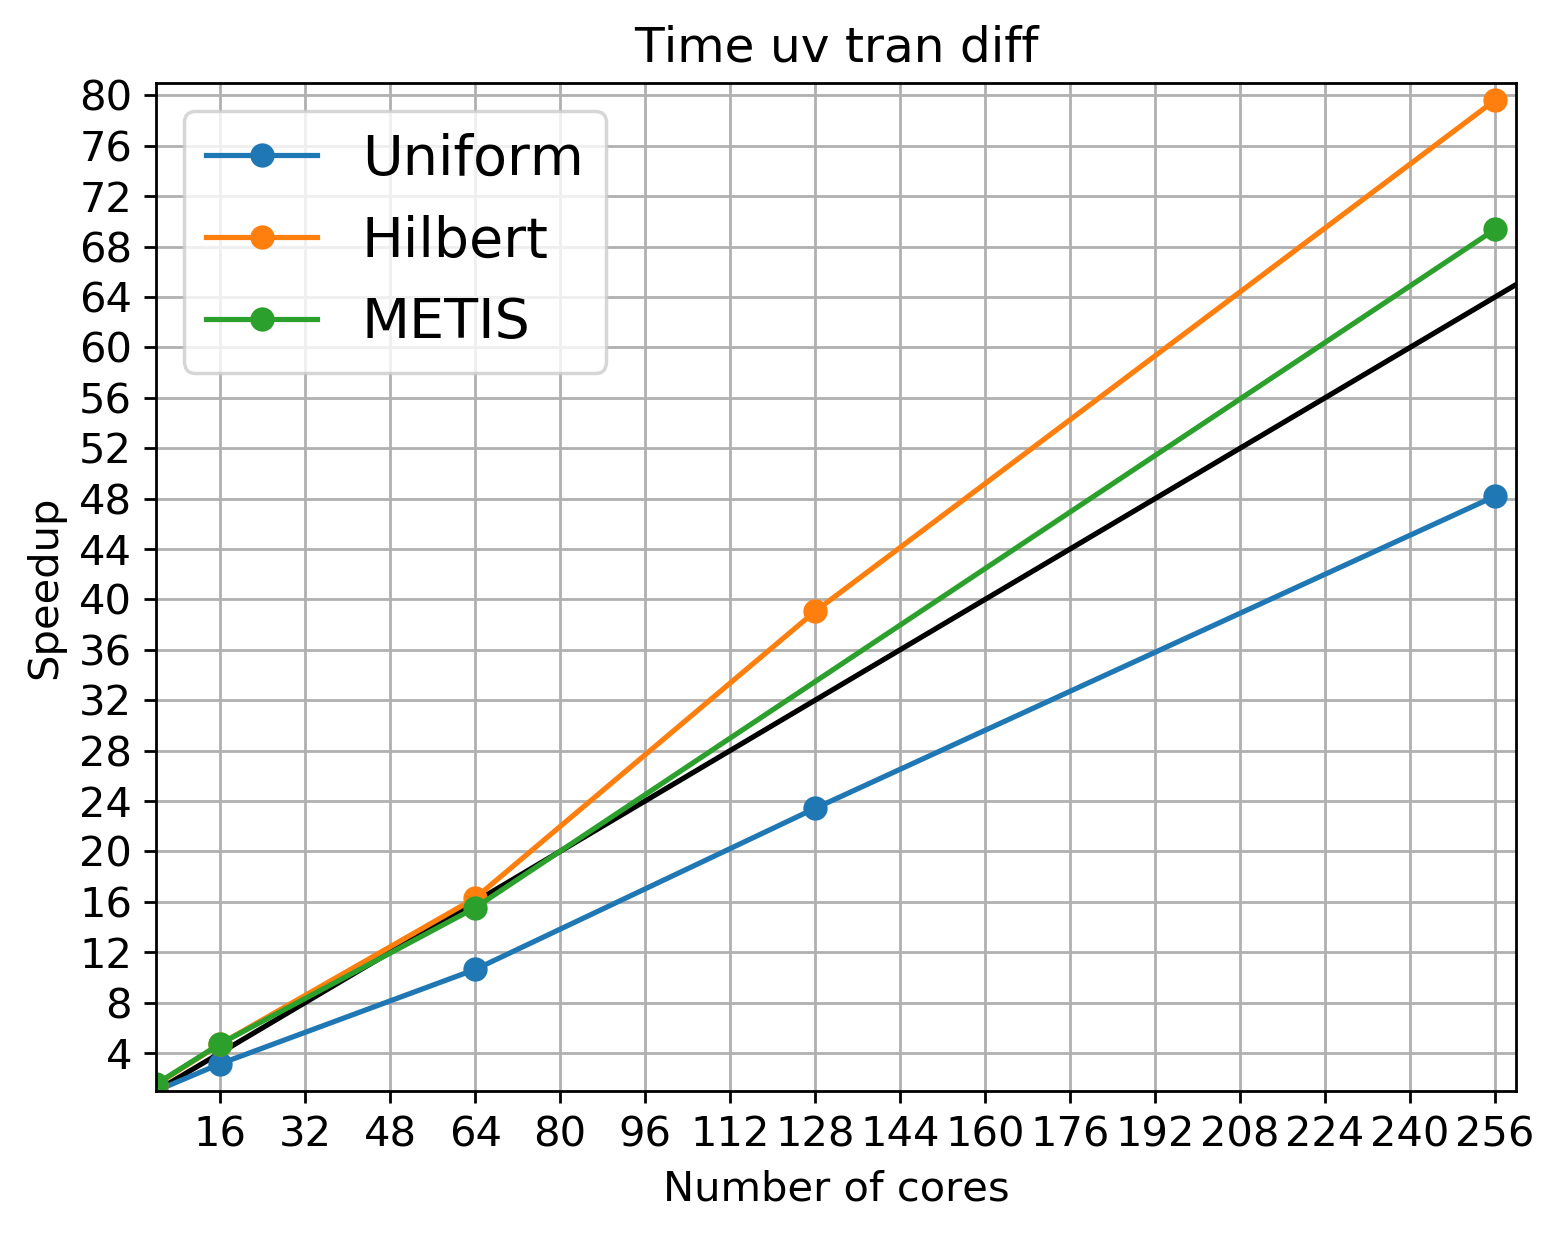
\includegraphics[width=1.0\linewidth]{plot4_upd_uv_tran_diff.png}}
    \end{minipage}
    \hfill
    \begin{minipage}[h]{0.48\linewidth}
    \center{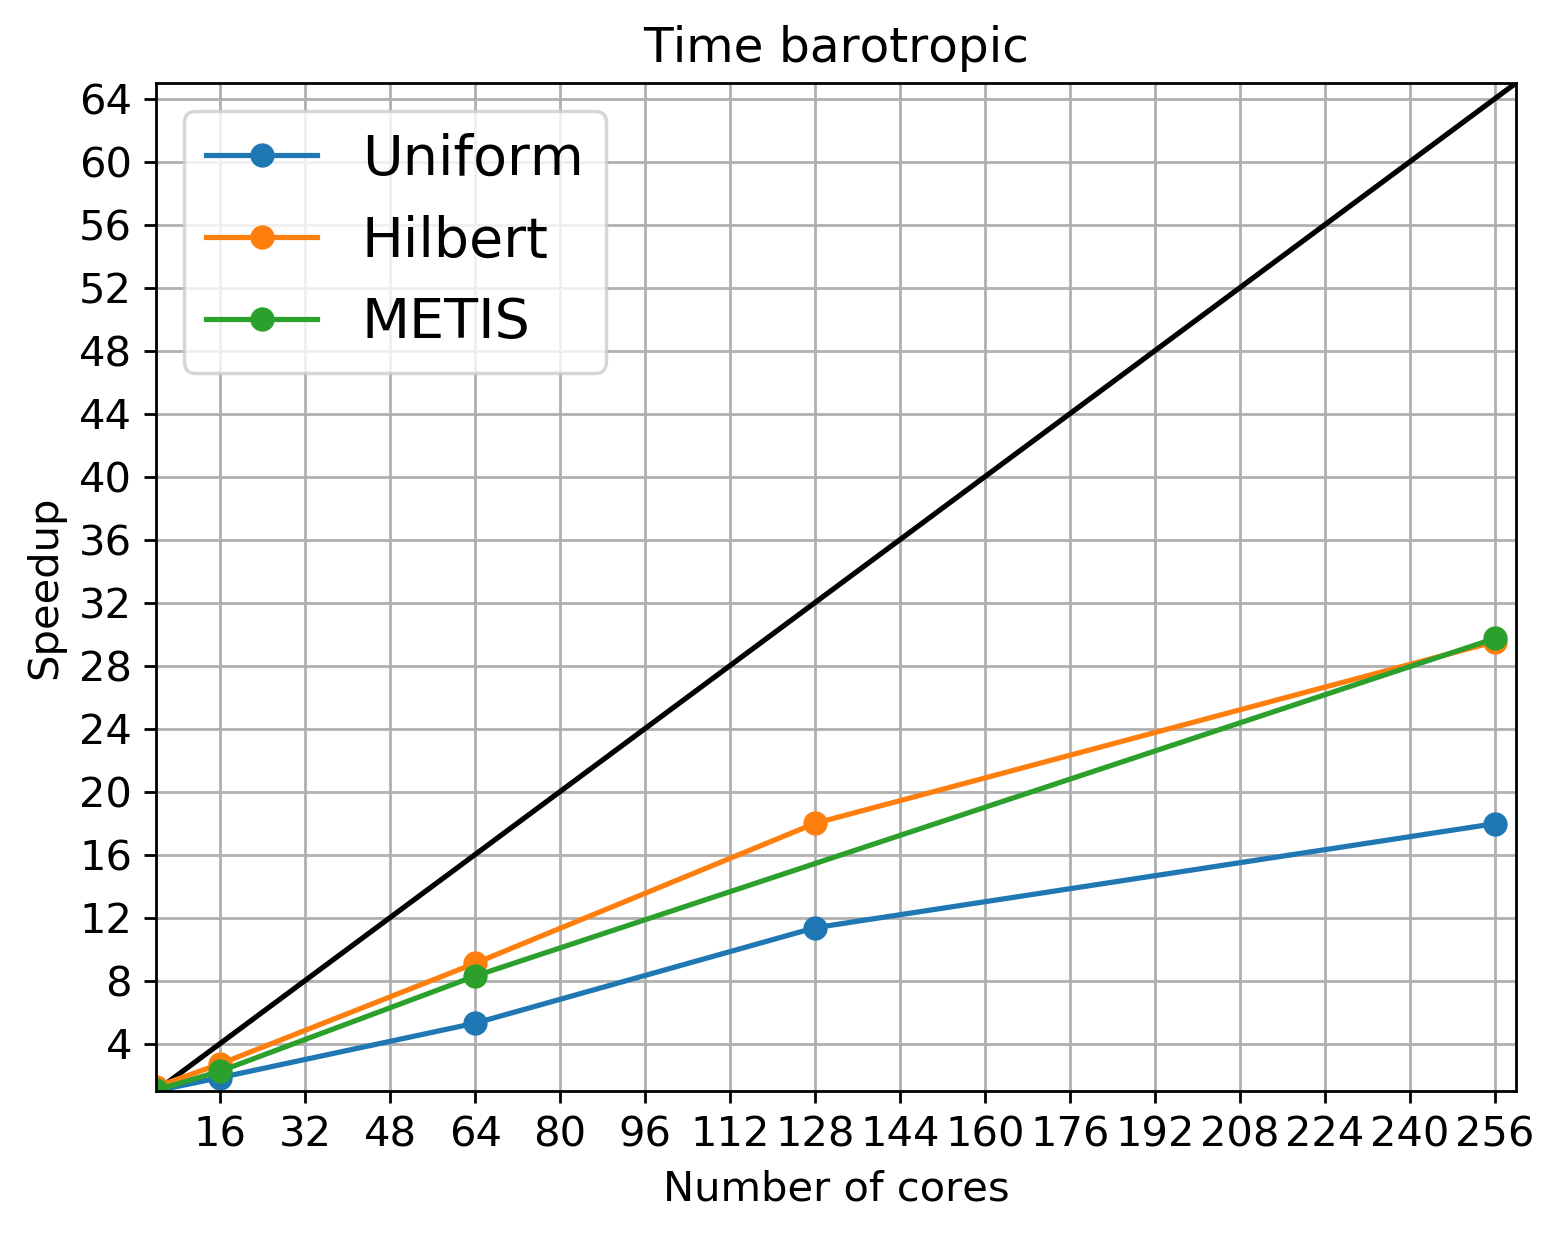
\includegraphics[width=1.0\linewidth]{plot4_upd_barotrop.png}}
    \end{minipage}
    \caption{Модель океана INMOM. Ускорение метода разбиения с использованием кривых Гильберта в сравнении с равномерным разбиением и с METIS. 1) Расчет переноса и диффузии для компонентов скорости. 2) Баротропная адаптация. 
    Чёрная линия соответствует линейному ускорению.}
    \label{fig:inmom_hilbert2}
    \end{figure}


	%В целом, для рассмотренной задачи выяснилось, что можно использовать как балансировку нагрузки с использованием кривых Гильберта так и METIS. 
    Отметим, что метод балансировки с использованием кривых Гильберта строит разбиения в несколько раз быстрее METIS, 
    но для рассматриваемой задачи это незначительно, т.к. расчетное время на порядок больше чем время построения разбиения. 
    Однако, алгоритм балансировки с использованием кривых Гильберта будет давать существенные преимущества по сравнению с METIS, когда задача будет упираться во время построения разбиения, 
    например, на очень большой расчетной области и с адаптивной сеткой.
    Также описанный алгоритм балансировки предпочтительнее чем METIS, так как он реализован непосредственно в модели
    и его реализация довольно простая в отличие от того, что реализовано в METIS.
    METIS - это библиотека для разбиений вообще произвольного вида, в ней реализованы довольно громоздкие методы, основанные на графах.
    А балансировка с использованием кривых Гильберта - это геометрический метод, который сильно проще и очень хорошо подходит именно для рассматриваемой задачи.  
    Используя описанный алгоритм балансировки нагрузки, у сигма-модели океана INMOM не будет привязки к сторонней библиотеке,
    поэтому дальнейшая разработка, поддержка и улучшения этого инструмента будут легче чем работа с METIS.
    
\begin{figure}[htb!]
	\center
	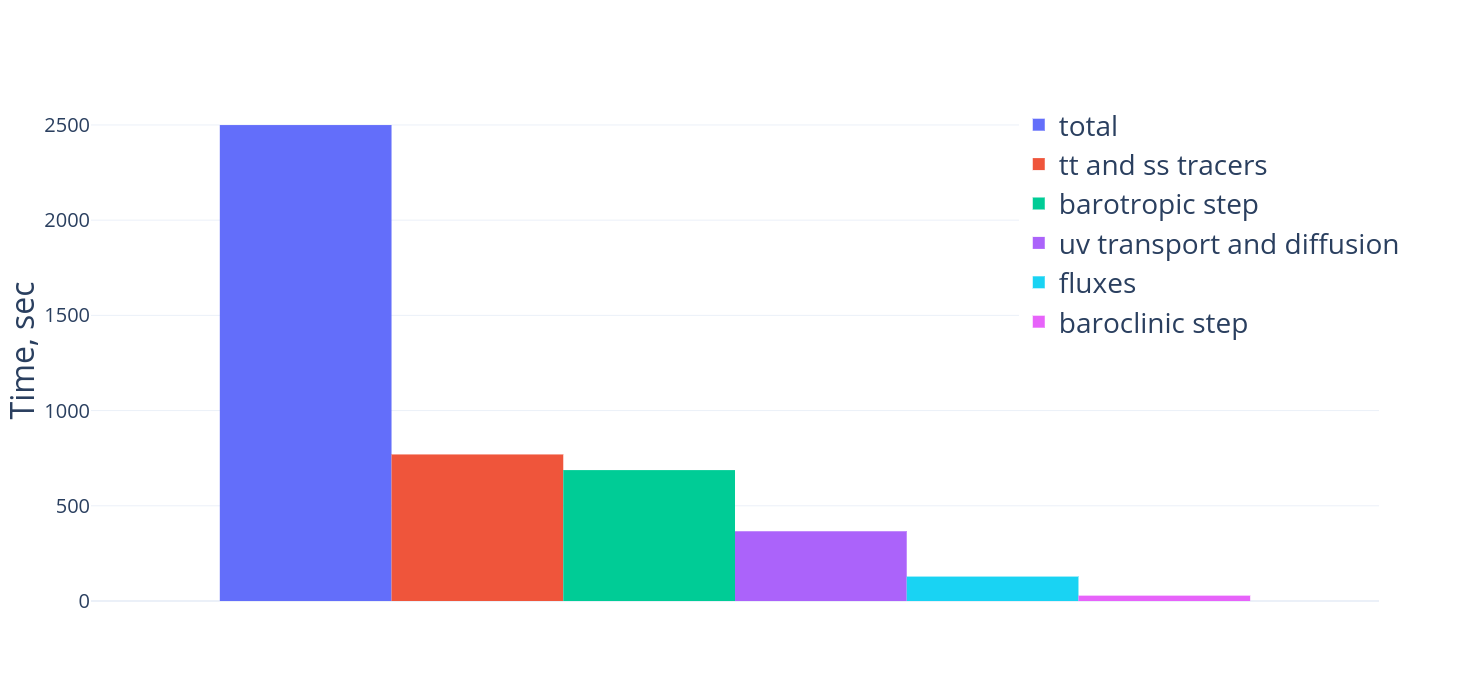
\includegraphics[scale = 0.3]{TimeModelSteps.png}
	\caption{Время работы разных блоков параллельной сигма-модели океана INMOM на 4 ядрах без балансировки нагрузки вычислений. 
	total - общее время работы модели; 
	tt and ss tracers - расчет температуры и солености; 
	barotropic - баротропная адаптация; 
	uv transport and diffusion - расчет переноса и диффузии для компонентов скорости;
	fluxes - расчет потоков на поверхности и дне; 
	baroclinic - бароклинная адаптация.}
	\label{fig:timemodelsteps}
\end{figure}

\FloatBarrier
           % Глава 3
\chapter*{Заключение}                       % Заголовок
\addcontentsline{toc}{chapter}{Заключение}  % Добавляем его в оглавление

%% Согласно ГОСТ Р 7.0.11-2011:
%% 5.3.3 В заключении диссертации излагают итоги выполненного исследования, рекомендации, перспективы дальнейшей разработки темы.
%% 9.2.3 В заключении автореферата диссертации излагают итоги данного исследования, рекомендации и перспективы дальнейшей разработки темы.
%% Поэтому имеет смысл сделать эту часть общей и загрузить из одного файла в автореферат и в диссертацию:

Диссертационная работа посвящена разработке и исследованию эффективности усовершенствованных версий модели общей циркуляции океана INMOM и модели мелкой воды для эффективного использования на массивно-параллельных многопроцессорных и гетерогенных вычислительных системах.

Основные результаты работы состоят в следующем.
%% Согласно ГОСТ Р 7.0.11-2011:
%% 5.3.3 В заключении диссертации излагают итоги выполненного исследования, рекомендации, перспективы дальнейшей разработки темы.
%% 9.2.3 В заключении автореферата диссертации излагают итоги данного исследования, рекомендации и перспективы дальнейшей разработки темы.
%\begin{enumerate}
%  \item На основе анализа \ldots
%  \item Численные исследования показали, что \ldots
%  \item Математическое моделирование показало \ldots
%  \item Для выполнения поставленных задач был создан \ldots
%\end{enumerate}

\begin{enumerate}
\item В работе разработана программная архитектура на принципе разделения обязанностей для модели общей циркуляции океана INMOM и, в частности,  модели мелкой воды. Разработанная программная архитектура предоставляет гибкий переход на гибридные модели параллельного программирования с использованием технологий MPI, OpenMP, CUDA.
\item На основе программной архитектуры были разработаны гибридные модели параллельного программирования для эффективного использования на массивно-параллельных многопроцессорных и гетерогенных вычислительных системах.
\item Разработан метод балансировки нагрузки вычислений на процессорах для улучшения масштабируемости и производительности моделей на высокопроизводительных вычислительных системах
\item Исследована масштабируемость и производительность предложенных методов на массивно-параллельных и гетерогенных вычислительных системах.
\end{enumerate}

В заключение автор выражает благодарность и большую признательность научному руководителю Дианскому~Н.\,А. за поддержку, помощь, обсуждение результатов и~научное руководство.
%Также автор благодарит Сидорова~А.\,А. и~Петрова~Б.\,Б. за помощь в~работе с~образцами, Рабиновича~В.\,В. за предоставленные образцы и~обсуждение результатов, Занудятину~Г.\,Г. и авторов шаблона *Russian-Phd-LaTeX-Dissertation-Template* за~помощь в оформлении диссертации. Автор также благодарит много разных людей и~всех, кто сделал настоящую работу автора возможной.

Работа сделана при поддержке научного гранта РФФИ № 20-31-90109.
      % Заключение
\include{Dissertation/acronyms}        % Список сокращений и условных обозначений
\chapter*{Словарь терминов}             % Заголовок
\addcontentsline{toc}{chapter}{Словарь терминов}  % Добавляем его в оглавление

\textbf{CPU} : Central processing unit

\textbf{GPU} : Graphics processing unit

\textbf{IPCC} : Intergovernmental Panel on Climate Change

\textbf{INMCM} : Institute of Numerical Mathematics Climate Model

\textbf{NEMO}: Nucleus for European Modeling of the Ocean

\textbf{POP}: Parallel Ocean Program

\textbf{HIROMB}: High Resolution Operational Model for the Baltic Sea

\textbf{INMОM} : Institute of Numerical Mathematics Ocean Model

\textbf{WRF} : Weather Research and Forecasting Model

\textbf{ИВМ РАН} : Институт Вычислительной Математики им. Г.И. Марчука Российской Академии Наук

\textbf{МЗС} : Модель земной системы

\textbf{МОЦО} : Модель общей циркуляции океана
      % Словарь терминов
\include{Dissertation/references}      % Список литературы
%% \include{Dissertation/lists}           % Списки таблиц и изображений (иллюстративный материал)

\setcounter{totalchapter}{\value{chapter}} % Подсчёт количества глав

%%% Настройки для приложений
\appendix
% Оформление заголовков приложений ближе к ГОСТ:
\setlength{\midchapskip}{20pt}
\renewcommand*{\afterchapternum}{\par\nobreak\vskip \midchapskip}
\renewcommand\thechapter{\Asbuk{chapter}} % Чтобы приложения русскими буквами нумеровались

%% \include{Dissertation/appendix}        % Приложения

\setcounter{totalappendix}{\value{chapter}} % Подсчёт количества приложений

\end{document}
